\documentclass[12pt]{article}
\usepackage[french]{babel}
\usepackage[utf8]{inputenc}
\usepackage[T1]{fontenc}
\usepackage{graphicx}
\graphicspath{{./}}
\usepackage{fancyhdr}
\usepackage{amsmath}
\usepackage{amssymb}
\usepackage{amsthm}
\usepackage{mathtools, bm}
\usepackage{cancel}
\usepackage{geometry}
\usepackage{xcolor}
\usepackage{enumitem}
\usepackage{booktabs}
\usepackage{titlesec}
\usepackage{tocloft}
\usepackage{tcolorbox}
\tcbuselibrary{theorems, breakable, skins}
\usepackage{hyperref}

\newcommand{\w}{\boldsymbol{w}}
\newcommand{\y}{\boldsymbol{y}}
\newcommand{\alt}{\bar\alpha_t}

\newcommand{\indep}{\perp\!\!\!\perp}
% ── Couleurs ──
\definecolor{sectioncolor}{rgb}{0.7, 0.1, 0.1}
\definecolor{subsectioncolor}{rgb}{0, 0.51, 0.58}
\definecolor{hypcolor}{RGB}{110, 70, 140}
\definecolor{proofgray}{RGB}{70, 70, 70}

\makeatletter
\let\ps@plain\ps@fancy
\makeatother

% ══════════════════════════════════════════════════════════
%   NUMÉROTATION : un compteur par type, lié à subsection
%   Format affiché : II.1.1, II.1.2, II.3.1, III.1.1 ...
% ══════════════════════════════════════════════════════════

% --- Compteur pour chaque type, reset à chaque subsection ---
\newcounter{cdef}[subsection]
\newcounter{cprop}[subsection]
\newcounter{cthm}[subsection]
\newcounter{chyp}[subsection]
\newcounter{cres}[subsection]

% --- Format d'affichage robuste ---
\makeatletter
\renewcommand{\thecdef}{\@Roman\c@section.\@arabic\c@subsection.\@arabic\c@cdef}
\renewcommand{\thecprop}{\@Roman\c@section.\@arabic\c@subsection.\@arabic\c@cprop}
\renewcommand{\thecthm}{\@Roman\c@section.\@arabic\c@subsection.\@arabic\c@cthm}
\renewcommand{\thechyp}{\@Roman\c@section.\@arabic\c@subsection.\@arabic\c@chyp}
\renewcommand{\thecres}{\@Roman\c@section.\@arabic\c@subsection.\@arabic\c@cres}
\makeatother

% ══════════════════════════════════════════════════════════
%   CADRES — fond blanc, style professionnel
% ══════════════════════════════════════════════════════════

% --- Définition (bleu-vert) ---
\newcommand{\definitiontitle}[1]{%
  \refstepcounter{cdef}%
  \textbf{\color{subsectioncolor}Définition \thecdef\ifx\\#1\\\else --- #1\fi}}
\newtcolorbox{definitionbox}[1][]{%
  enhanced, breakable, colback=white, colframe=subsectioncolor,
  boxrule=0.6pt, arc=0pt, outer arc=0pt,
  left=3mm, right=3mm, top=0mm, bottom=2mm,
  before upper={\definitiontitle{#1}\par\smallskip}}

% --- Proposition (bleu-vert, trait plus épais) ---
\newcommand{\propositiontitle}[1]{%
  \refstepcounter{cprop}%
  \textbf{\color{subsectioncolor}Proposition \thecprop\ifx\\#1\\\else --- #1\fi}}
\newtcolorbox{propositionbox}[1][]{%
  enhanced, breakable, colback=white, colframe=subsectioncolor,
  boxrule=0.8pt, arc=0pt, outer arc=0pt,
  left=3mm, right=3mm, top=0mm, bottom=2mm,
  before upper={\propositiontitle{#1}\par\smallskip}}

% --- Théorème (rouge) ---
% \newcommand{\theoremtitle}[1]{%
%   \refstepcounter{cthm}%
%   \textbf{\color{sectioncolor}Théorème \thecthm\ifx\\#1\\\else --- #1\fi}}
% \newtcolorbox{theorembox}[1][]{%
%   enhanced, breakable, colback=white, colframe=sectioncolor,
%   boxrule=1pt, arc=0pt, outer arc=0pt,
%   left=3mm, right=3mm, top=0mm, bottom=2mm,
%   before upper={\theoremtitle{#1}\par\smallskip}}

\newcommand{\theoremtitle}[1]{%
    \refstepcounter{cres}%
    \textbf{\color{sectioncolor}Théorème \thecres\ifx\\#1\\\else --- #1\fi}}
\newtcolorbox{theorembox}[1][]{%
  enhanced, breakable, colback=white, colframe=sectioncolor,
  boxrule=1.2pt, arc=0pt, outer arc=0pt,
  borderline={0.4pt}{1.8pt}{sectioncolor},
  left=3mm, right=3mm, top=0mm, bottom=2mm,
  before upper={\theoremtitle{#1}\par\smallskip}}


% --- Résultat (rouge, double filet) ---
\newcommand{\resulttitle}[1]{%
  \refstepcounter{cres}%
  \textbf{\color{sectioncolor}Résultat \thecres\ifx\\#1\\\else --- #1\fi}}
\newtcolorbox{resultbox}[1][]{%
  enhanced, breakable, colback=white, colframe=sectioncolor,
  boxrule=1.2pt, arc=0pt, outer arc=0pt,
  borderline={0.4pt}{1.8pt}{sectioncolor},
  left=3mm, right=3mm, top=0mm, bottom=2mm,
  before upper={\resulttitle{#1}\par\smallskip}}

% --- Hypothèses (violet) ---
\newcommand{\hypothesetitle}[1]{%
  \refstepcounter{chyp}%
  \textbf{\color{hypcolor}Hypothèses \thechyp\ifx\\#1\\\else --- #1\fi}}
\newtcolorbox{hypothesebox}[1][]{%
  enhanced, breakable, colback=white, colframe=hypcolor,
  boxrule=0.6pt, arc=0pt, outer arc=0pt,
  left=3mm, right=3mm, top=0mm, bottom=2mm,
  before upper={\hypothesetitle{#1}\par\smallskip}}

% --- Remarque (pas numérotée, gris clair) ---
\newtcolorbox{remarkbox}[1][]{%
  enhanced, breakable, colback=white, colframe=subsectioncolor!50,
  boxrule=0.3pt, arc=0pt, outer arc=0pt,
  left=3mm, right=3mm, top=0mm, bottom=2mm,
  before upper={\textit{\color{subsectioncolor!70!black}Remarque\ifx\\#1\\\else --- #1\fi}\par\smallskip}}

  \newtcolorbox{rappelbox}[1][]{%
  enhanced, breakable, colback=white, colframe=subsectioncolor!50,
  boxrule=0.3pt, arc=0pt, outer arc=0pt,
  left=3mm, right=3mm, top=0mm, bottom=2mm,
  before upper={\textit{\color{subsectioncolor!70!black}Rappel\ifx\\#1\\\else --- #1\fi}\par\smallskip}}
% ── Preuve : italique gris + ■ en bas à droite ──
\renewcommand{\qedsymbol}{$\blacksquare$}
\renewenvironment{proof}[1][\proofname]{%
  \par\medskip\noindent
  \textit{\color{proofgray}#1.}\enspace\ignorespaces
}{\hfill\qedsymbol\par\medskip}
\renewcommand{\proofname}{Preuve}

% ── Table des matières ──
\renewcommand{\cftsecfont}{\color{sectioncolor}\bfseries}
\renewcommand{\cftsecpagefont}{\color{sectioncolor}\bfseries}
\setlength{\cftsecnumwidth}{2.5em}
\cftsetindents{section}{0em}{3em}
\renewcommand{\cftsubsecfont}{\color{subsectioncolor}\bfseries}
\renewcommand{\cftsubsecpagefont}{\color{subsectioncolor}\bfseries}
\setlength{\cftsubsecnumwidth}{3em}
\cftsetindents{subsection}{2em}{4em}
\renewcommand{\cftsubsubsecfont}{\color{subsectioncolor}}
\cftsetindents{subsubsection}{4em}{4.5em}
\renewcommand{\cftsubsubsecpagefont}{\color{subsectioncolor}}
\renewcommand{\cftpartfont}{\color{sectioncolor}\bfseries\Large}
\renewcommand{\cftpartpagefont}{\color{sectioncolor}\bfseries\Large}
\cftsetindents{part}{0em}{4em}
\renewcommand{\cftbeforepartskip}{1em}
\renewcommand{\cftpartfont}{\color{sectioncolor}\bfseries\Large\rule{\linewidth}{0.4pt}\\}
\renewcommand{\cftpartpresnum}{}
\setlength{\cftpartnumwidth}{0em}
\renewcommand{\thepart}{}


\hypersetup{linktoc=all, colorlinks=true,
  linkcolor=sectioncolor, citecolor=subsectioncolor, urlcolor=subsectioncolor, pdfborder={0 0 0}}

\geometry{a4paper, top=2cm, bottom=2cm, left=2cm, right=2cm,
  headheight=36.0976pt, includeheadfoot}

\pagestyle{fancy}\fancyhf{}
\fancyhead[R]{
\includegraphics[width=2.5cm]{images.png}}
\fancyhead[L]{
\includegraphics[width=3.3cm]{satie-cnrs.png}}
\fancyfoot[L]{Gatien Séguy}\fancyfoot[R]{\thepage}
\renewcommand{\headrulewidth}{0.4pt}\renewcommand{\footrulewidth}{0.4pt}

\titleformat{\part}[display]
  {\Huge\bfseries\centering\color{sectioncolor}}{}{0pt}
  {\rule{\textwidth}{1pt}\\\vspace{0.2em}}[\vspace{0.2em}\rule{\textwidth}{1pt}]
\titlespacing*{\part}{0pt}{-60pt}{20pt}
\titleformat{\section}{\normalfont\Large\bfseries\color{sectioncolor}}{\thesection}{1em}{}
\titlespacing*{\section}{0pt}{3.5ex plus 1ex minus .2ex}{2.3ex plus .2ex}
\renewcommand{\thesection}{\Roman{section}}
\titleformat{\subsection}{\normalfont\large\bfseries\color{subsectioncolor}}{\thesubsection}{1em}{}

\begin{document}

\begin{titlepage}
\thispagestyle{empty}

\vspace*{-3.2cm}

\begin{center}
    % ── Logos côte à côte ──
    \begin{minipage}{0.24\textwidth}\centering
        
\includegraphics[width=1\linewidth]{Logo_ENS_leger(1).jpg}
    \end{minipage}\hfill
    \begin{minipage}{0.24\textwidth}\centering
        
\includegraphics[width=1\linewidth]{logo_univPS.png}
    \end{minipage}\hfill
    \begin{minipage}{0.24\textwidth}\centering
        
\includegraphics[width=0.7\linewidth]{logo_satie.png}
    \end{minipage}\hfill
    \begin{minipage}{0.24\textwidth}\centering
        
\includegraphics[width=0.7\linewidth]{logo_cnrs.png}
    \end{minipage}

    \vspace{0.6cm}

    % ── Nom de l'école ──
    {\Large \textbf{ÉCOLE NORMALE SUPÉRIEURE PARIS-SACLAY}}\\[0.15cm]
    {\normalsize Université Paris-Saclay}\\
    \vspace{0.5cm}
    
    {\Large \textbf{SATIE}}\\[0.15cm]
    {\normalsize Laboratoire des systèmes et applications des technologies de l'information et de l'énergie}
    \vspace{0.5cm}

    % ── Bloc titre encadré ──
    {\color{black}\rule{1\textwidth}{1.2pt}}
    {\color{black}\rule{0.9\textwidth}{0.8pt}}

    \vspace{0.45cm}

    {\Huge \color{black} \textbf{Modèles de diffusion appliqués aux problèmes inverses : estimation variationnelle bayésienne des hyperparamètres}}

    \vspace{0.35cm}
    
    {\Huge Gatien Séguy}

    \vspace{0.35cm}

    {\color{black}\rule{0.9\textwidth}{0.8pt}}
    {\color{black}\rule{1\textwidth}{1.2pt}}

    \vspace{0.5cm}
  
    % ── Informations ──
    \renewcommand{\arraystretch}{1.5}
    \begin{tabular}{r@{\hspace{0.8em}:\hspace{0.8em}}l}
    \textbf{Laboratoire }  & SATIE -- ENS Paris-Saclay\\
    \textbf{Superviseur}    & Thomas Rodet (SATIE -- CNRS)\\
    \textbf{Date de début}           & 1\ier avril 2026 \\
    \textbf{Date de fin}           & 15 juillet 2026 \\
    \end{tabular}
    \renewcommand{\arraystretch}{1}

    \vspace{0.3cm}
    \begin{center}
    \textbf{RÉSUMÉ}
    \end{center}
    \begin{minipage}{0.88\textwidth}\small
     Ce stage porte sur la résolution de problèmes inverses en imagerie à l'aide de modèles de diffusion génératifs. Nous formalisons d'abord le processus de diffusion forward comme une équation différentielle stochastique, établissons la formule de Tweedie reliant le score à l'estimateur optimal, et présentons les méthodes existantes de reconstruction conditionnelle (DPS, $\Pi$GDM). Nous proposons ensuite une approche combinant le cadre $\Pi$GDM avec l'inférence variationnelle bayésienne (algorithme EMG-VBA) pour estimer automatiquement les hyperparamètres du modèle ($\tau_r$, $\tau_b$) plutôt que de les fixer manuellement. Contrairement aux méthodes classiques qui décomposent le score conditionnel en score a priori et score de vraisemblance, notre formulation fournit le score conditionnel total en forme fermée. L'optimisation est menée dans l'espace des mesures de probabilité via des mises à jour multiplicatives (Radon-Nikodym).
    \end{minipage}
    \vfill
\end{center}
\vfill
\begin{center}
    {\color{sectioncolor}\rule{0.3\textwidth}{0.4pt}}\\[0.35cm]
    {\small\color{proofgray} Stage de recherche -- Master 2 FESup Intranet}
\end{center}


\vspace*{-1.5cm}
%\noindent{\color{black}\rule{\textwidth}{2pt}}
\end{titlepage}

\setcounter{page}{2}\newpage\vspace*{0.5cm}\tableofcontents\newpage

\part{Modèles de Diffusion Génératifs}

\section{Introduction}

Un modèle de diffusion génératif repose sur une idée simple : dégrader progressivement les données en ajoutant du bruit, puis apprendre à inverser cette destruction. Le \textbf{processus directe} (forward) corrompt une donnée réelle par des ajouts successifs de bruit gaussien jusqu'à obtenir du bruit pur. Le \textbf{processus inverse} (reverse), guidé par un réseau de neurones, fait le chemin inverse.
Ce compte rendu retrace le cheminement entre autres mathématique. On formalise le processus forward comme une SDE, on la résout sous trois variantes, on introduit la formule de Tweedie et le score, puis on montre comment guider la génération par des mesures $y$ pour résoudre des problèmes inverses en imagerie par exemple (IRM, super-résolution, inpainting).
\section{Processus de Diffusion Forward}

\subsection{Le mouvement Brownien}

Le mouvement Brownien modélise un bruit continu, gaussien, à incréments indépendants. C'est exactement ce qu'il faut pour corrompre progressivement une image.

\begin{definitionbox}[Processus de Wiener standard]
\label{def:wiener}
Les variables aléatoires $(W_t)_{t \geq 0}$ à valeurs dans $\mathbb{R}^n$ est un \textbf{processus de Wiener standard} si :
\begin{enumerate}[label=(\roman*)]
    \item $W_0 = 0$,
    \item les incréments sont indépendants : pour $0 \leq t_1 < \cdots < t_k$, les variables aléatoires (v.a.)\ $W_{t_2} - W_{t_1}, \ldots, W_{t_k} - W_{t_{k-1}}$ sont indépendantes,
    \item les incréments sont gaussiens : $W_t - W_s \sim \mathcal{N}(0, (t-s)\, I_n)$ pour $0 \leq s < t$,
    \item les trajectoires $t \mapsto W_t$ sont continues.
\end{enumerate}
\end{definitionbox}

La propriété (iii) est cruciale : la variance des incréments est proportionnelle au temps, donc l'écart-type croît en $\sqrt{t}$. C'est cette propriété qui fait apparaître les $\sqrt{\cdot}$ dans les formules de diffusion.

\subsection{Formulation SDE (Stochastic Differential Equation)}

On combine un décalage (drift) déterministe et un bruit brownien dans une équation différentielle stochastique.

\begin{definitionbox}[SDE forward]
\label{def:sde}
Le processus forward est défini par :
\begin{equation}
    \boxed{\mathrm{d}X_t = f(X_t, t)\,\mathrm{d}t + g(t)\,\mathrm{d}W_t, \qquad X_0 \sim p_{\text{data}}}
    \label{eq:sde_forward}
\end{equation}
où $f(X_t, t)$ est le \textbf{drift}, $g(t)$ le \textbf{coefficient de diffusion}, et $W_t$ un mouvement Brownien standard (Définition \ref{def:wiener}).
\end{definitionbox}

L'objectif est de résoudre cette SDE : exprimer la loi de $X_t | X_0$. Trois outils de calcul stochastique sont nécessaires.

\subsection{Outils de calcul stochastique}

\begin{propositionbox}[Isométrie d'Itô]
\label{prop:ito}
Soit $g : [0,T] \to \mathbb{R}$ déterministe avec $\int_0^T g(s)^2\, \mathrm{d}s < \infty$. Alors :
\begin{equation}
    \mathbb{E}\!\left[\left(\int_0^T g(s)\, \mathrm{d}W_s\right)^{\!2}\right] = \int_0^T g(s)^2\, \mathrm{d}s
    \label{eq:ito_isometry}
\end{equation}
\end{propositionbox}

\begin{proof}

\textbf{Étape 1 : approximation en escalier.} Soit $\pi = \{0 = t_0 < t_1 < \cdots < t_N = T\}$ une partition de $[0,T]$. On approche l'intégrale stochastique par :
\[
I_\pi :=\int_0^T g(s) dW_s = \sum_{k=0}^{N-1} g(t_k)\,(W_{t_{k+1}} - W_{t_k})
\]

\textbf{Étape 2 : développement de $I_\pi^2$.}
\[
I_\pi^2 = \sum_{k=0}^{N-1} \sum_{j=0}^{N-1} g(t_k)\,g(t_j)\,(W_{t_{k+1}} - W_{t_k})(W_{t_{j+1}} - W_{t_j})
\]

\textbf{Étape 3 : annulation des termes croisés.} Pour $k \neq j$, les incréments $(W_{t_{k+1}} - W_{t_k})$ et $(W_{t_{j+1}} - W_{t_j})$ sont indépendants par la Définition \ref{def:wiener}~(ii). Comme $g$ est déterministe :
\[
\mathbb{E}\!\left[g(t_k)\,g(t_j)\,(W_{t_{k+1}} - W_{t_k})(W_{t_{j+1}} - W_{t_j})\right] = g(t_k)\,g(t_j)\, \underbrace{\mathbb{E}[W_{t_{k+1}} - W_{t_k}]}_{= 0} \cdot \mathbb{E}[W_{t_{j+1}} - W_{t_j}] = 0
\]
où l'on a utilisé $\mathbb{E}[W_t - W_s] = 0$ par la Définition \ref{def:wiener}~(iii).

\textbf{Étape 4 : termes diagonaux.} Pour $k = j$ :
\[
\mathbb{E}\!\left[g(t_k)^2\,(W_{t_{k+1}} - W_{t_k})^2\right] = g(t_k)^2 \cdot \underbrace{\mathbb{E}\!\left[(W_{t_{k+1}} - W_{t_k})^2\right]}_{= \Delta t_k} = g(t_k)^2\, \Delta t_k
\]
où l'on a utilisé $\mathrm{Var}(W_{t_{k+1}} - W_{t_k}) = t_{k+1} - t_k$ par la Définition \ref{def:wiener}~(iii).

\textbf{Étape 5 : passage à la limite.}
\[
\mathbb{E}[I_\pi^2] = \sum_{k=0}^{N-1} g(t_k)^2\, \Delta t_k \;\xrightarrow{ \Delta t_k \to 0 \quad \forall k }\; \int_0^T g(s)^2\, \mathrm{d}s
\]
par définition de l'intégrale de Riemann.
\end{proof}



De même, l'espérance est nulle : $\mathbb{E}[I_\pi] = \sum_k g(t_k) \cdot \mathbb{E}[W_{t_{k+1}} - W_{t_k}] = 0$ par la Définition \ref{def:wiener} (iii).

\begin{propositionbox}[Gaussianité de l'intégrale stochastique]
\label{prop:gauss}
Si $g : [0,T] \to \mathbb{R}$ est déterministe :
\begin{equation}
    \int_0^T g(s)\, \mathrm{d}W_s \sim \mathcal{N}\!\left(0,\; \int_0^T g(s)^2\, \mathrm{d}s\right)
\end{equation}
En dimension $n$ : $\int_0^T g(s)\, \mathrm{d}W_s \sim \mathcal{N}\!\left(0, \left(\int_0^T g(s)^2\, \mathrm{d}s\right) I_n\right)$.
\end{propositionbox}

  \begin{proof}







\textbf{Étape 1 :} L'approximation $I_\pi = \sum_{k=0}^{N-1} g(t_k)(W_{t_{k+1}} - W_{t_k})$ est une combinaison linéaire de variables gaussiennes indépendantes (les $W_{t_{k+1}} - W_{t_k}$ sont indépendants par la Définition \ref{def:wiener} (ii), gaussiens par (iii), et les $g(t_k)$ sont déterministes). Une combinaison linéaire de gaussiennes indépendantes est gaussienne.

\textbf{Étape 2 :} $I_\pi \sim \mathcal{N}(0,\, \sum_k g(t_k)^2 \Delta t_k)$ (espérance nulle, variance par la Proposition \ref{prop:ito}).

\textbf{Étape 3 :} La limite en loi d'une suite de gaussiennes est gaussienne (la famille $\mathcal{N}(\mu_n, \sigma_n^2)$ est fermée pour la convergence en loi quand $\mu_n \to \mu$ et $\sigma_n^2 \to \sigma^2$). D'où le résultat.

\textbf{Étape 4 :} En dimension $n$ : les composantes $W_t^{(1)}, \ldots, W_t^{(n)}$ sont des browniens réels indépendants (Définition \ref{def:wiener}). Chaque composante $\int_0^T g(s)\, \mathrm{d}W_s^{(i)}$ est donc gaussienne centrée de variance $\int g^2\, \mathrm{d}s$, et les composantes sont indépendantes.
\end{proof}

\begin{propositionbox}[Formule d'Itô]
\label{prop:itoformula}
Soit $X_t$ un processus d'Itô $\mathrm{d}X_t = \mu_t\,\mathrm{d}t + \sigma_t\,\mathrm{d}W_t$ et $f(x,t) \in C^{2} \times C^{1}$ :
\begin{equation}
    \mathrm{d}f(X_t, t) = \frac{\partial f}{\partial t}\,\mathrm{d}t + \frac{\partial f}{\partial x}\,\mathrm{d}X_t + \frac{1}{2}\frac{\partial^2 f}{\partial x^2}\,\sigma_t^2\,\mathrm{d}t
\end{equation}
\end{propositionbox}

Le dernier terme vient de $(\mathrm{d}W_t)^2 = \mathrm{d}t$ : c'est le Taylor stochastique à l'ordre 2. Ces trois outils en main, on résout la SDE.

\section{Résolution de la SDE : trois variantes}

Trois formulations coexistent. Elles diffèrent par $f$ et $g$, mais conduisent toutes à : $X_t = \alpha_t X_0 + \sigma_t Z$, un mélange entre signal ($\alpha_t$ décroît) et bruit ($\sigma_t$ croît).

\subsection{Variance Exploding (VE)}

\begin{hypothesebox}[VE]
\label{hyp:ve}
$f(X_t, t) = 0$ et $g(t) = \sqrt{\mathrm{d}\sigma_t^2/\mathrm{d}t}$, avec $\sigma_0 = 0$ et $(\sigma_t)$ croissant.
\end{hypothesebox}

\begin{resultbox}[Loi marginale VE]
\label{res:ve}
\begin{equation}
    \boxed{X_t = X_0 + \sigma_t\, Z, \qquad Z \sim \mathcal{N}(0, I_n)}
    \label{eq:ve_marginal}
\end{equation}
avec $\alpha_t = 1$ et $\sigma_t^2 = \int_0^t g(s)^2\, \mathrm{d}s$.
\end{resultbox}

  \begin{proof}







\textbf{Étape 1 : intégration directe.} Sous les Hypothèses \ref{hyp:ve}, la SDE \eqref{eq:sde_forward} se réduit à $\mathrm{d}X_t = g(t)\, \mathrm{d}W_t$. En intégrant de $0$ à $t$ :
\[
X_t = X_0 + \int_0^t g(s)\, \mathrm{d}W_s
\]

\textbf{Étape 2 : espérance conditionnelle.} Sachant $X_0$, l'intégrale stochastique est une fonctionnelle du brownien $W$, indépendante de $X_0$. Par la Proposition \ref{prop:ito} (espérance nulle) :
\[
\mathbb{E}[X_t \mid X_0] = X_0 + \mathbb{E}\!\left[\int_0^t g(s)\, \mathrm{d}W_s\right] = X_0
\]

\textbf{Étape 3 : variance conditionnelle.} Par l'isométrie d'Itô (Proposition \ref{prop:ito}), $g$ étant déterministe :
\[
\mathrm{Var}(X_t \mid X_0) = \mathbb{E}\!\left[\left(\int_0^t g(s)\, \mathrm{d}W_s\right)^{\!2}\right] = \int_0^t g(s)^2\, \mathrm{d}s = \int_0^t \frac{\mathrm{d}\sigma_s^2}{\mathrm{d}s}\, \mathrm{d}s = \sigma_t^2 - \underbrace{\sigma_0^2}_{=0} = \sigma_t^2
\]

\textbf{Étape 4 : identification de la loi.} Par la Proposition \ref{prop:gauss} (gaussianité de l'intégrale stochastique à noyau déterministe, puis généralisation à $\mathbb{R}^n$), on a :
\[
\int_0^t g(s)\, \mathrm{d}W_s \sim \mathcal{N}(0,\, \sigma_t^2\, I_n) \;=\; \sigma_t\, Z, \quad Z \sim \mathcal{N}(0, I_n)
\]
D'où $X_t = X_0 + \sigma_t\, Z$.
\end{proof}

La variance totale de $X_t$ vaut $\mathrm{Var}(X_0) + \sigma_t^2$ : elle croît sans borne, d'où le nom \textit{Variance Exploding}.


\subsection{Variance Preserving (VP) --- Ornstein--Uhlenbeck}

\begin{hypothesebox}[VP]
\label{hyp:vp}
$f(X_t, t) = -X_t$ et $g(t) = \sqrt{2}$.
\end{hypothesebox}

La SDE $\mathrm{d}X_t = -X_t\,\mathrm{d}t + \sqrt{2}\,\mathrm{d}W_t$ est le processus d'Ornstein--Uhlenbeck : le drift $-X_t$ tire vers l'origine, le bruit repousse.

\begin{resultbox}[Loi marginale VP]
\label{res:vp}
\begin{equation}
    \boxed{X_t = e^{-t} X_0 + \sqrt{1 - e^{-2t}}\, Z, \qquad Z \sim \mathcal{N}(0, I_n)}
    \label{eq:vp_marginal}
\end{equation}
avec $\alpha_t = e^{-t}$ et $\sigma_t = \sqrt{1 - e^{-2t}}$.
\end{resultbox}

  \begin{proof}







\textbf{Étape 1 : changement de variable.} On pose $Y_t = e^t X_t$ et on applique la formule d'Itô (Proposition \ref{prop:itoformula}) avec $f(x,t) = e^t x$ :
\[
\frac{\partial f}{\partial t} = e^t x, \qquad \frac{\partial f}{\partial x} = e^t, \qquad \frac{\partial^2 f}{\partial x^2} = 0
\]
\begin{align}
    \mathrm{d}Y_t &= e^t X_t\,\mathrm{d}t + e^t\,\mathrm{d}X_t + \underbrace{\frac{1}{2} \cdot 0 \cdot (\sqrt{2})^2}_{=0}\,\mathrm{d}t \nonumber\\
    &= e^t X_t\,\mathrm{d}t + e^t\bigl(-X_t\,\mathrm{d}t + \sqrt{2}\,\mathrm{d}W_t\bigr) \nonumber\\
    &= \cancel{e^t X_t\,\mathrm{d}t} - \cancel{e^t X_t\,\mathrm{d}t} + \sqrt{2}\, e^t\, \mathrm{d}W_t = \sqrt{2}\, e^t\, \mathrm{d}W_t
\end{align}
Le drift a disparu : $Y_t$ suit un brownien pur de coefficient $\sqrt{2}\, e^t$.

\textbf{Étape 2 : intégration.}
\[
Y_t = Y_0 + \sqrt{2}\int_0^t e^s\, \mathrm{d}W_s = X_0 + \sqrt{2}\int_0^t e^s\, \mathrm{d}W_s
\]
En divisant par $e^t$ :
\[
X_t = e^{-t}\, X_0 + \sqrt{2}\, e^{-t}\int_0^t e^s\, \mathrm{d}W_s
\]

\textbf{Étape 3 : espérance.} L'intégrale stochastique est d'espérance nulle (Proposition \ref{prop:ito}) :
\[
\mathbb{E}[X_t \mid X_0] = e^{-t}\, X_0
\]

\textbf{Étape 4 : variance.} Le noyau $\tilde{g}(s) = \sqrt{2}\, e^s$ est déterministe. Par l'isométrie d'Itô (Proposition \ref{prop:ito}) :
\begin{align}
    \mathrm{Var}(X_t \mid X_0) &= e^{-2t} \cdot \mathbb{E}\!\left[\left(\sqrt{2}\int_0^t e^s\, \mathrm{d}W_s\right)^{\!2}\right] = e^{-2t} \cdot 2\int_0^t e^{2s}\, \mathrm{d}s \nonumber\\
    &= e^{-2t} \cdot 2 \cdot \frac{e^{2t} - 1}{2} = 1 - e^{-2t}
\end{align}

\textbf{Étape 5 : identification et vérification.} Par la Proposition \ref{prop:gauss} : $X_t \mid X_0 \sim \mathcal{N}(e^{-t} X_0,\; (1-e^{-2t})\, I_n)$. On vérifie : $\alpha_t^2 + \sigma_t^2 = e^{-2t} + 1 - e^{-2t} = 1$. Si $\mathrm{Var}(X_0) = 1$, alors $\mathrm{Var}(X_t) = 1$ à tout instant d'où le nom \textit{Variance Preserving}.
\end{proof}


\subsection{DDPM (Denoising Diffusion Probabilistic Models)--- formulation discrète}

\begin{definitionbox}[Processus forward DDPM]
\label{def:ddpm}
Chaîne de Markov : $q(X_t | X_{t-1}) = \mathcal{N}(\sqrt{1-\beta_t}\, X_{t-1},\, \beta_t I_n)$ avec $\alpha_t = 1-\beta_t$ et $\bar\alpha_t = \prod_{s=1}^t \alpha_s$.
\end{definitionbox}

\begin{resultbox}[Loi marginale DDPM]
\label{res:ddpm}
\begin{equation}
    \boxed{X_t = \sqrt{\bar\alpha_t}\, X_0 + \sqrt{1-\bar\alpha_t}\, Z, \qquad Z \sim \mathcal{N}(0, I_n)}
    \label{eq:ddpm_marginal}
\end{equation}
\end{resultbox}

  \begin{proof}







Par récurrence sur $t$.

\textbf{Initialisation} ($t=1$). Par la Définition \ref{def:ddpm} : $X_1 = \sqrt{\alpha_1}\, X_0 + \sqrt{\beta_1}\, \epsilon_1$ avec $\epsilon_1 \sim \mathcal{N}(0, I_n)$. Comme $\bar\alpha_1 = \alpha_1$ et $1 - \bar\alpha_1 = \beta_1$, c'est bien la forme attendue.

\textbf{Hérédité.} Supposons $X_t = \sqrt{\bar\alpha_t}\, X_0 + \sqrt{1-\bar\alpha_t}\, Z_t$ avec $Z_t \sim \mathcal{N}(0, I_n)$.

\textit{Étape 1 : substitution.} Par la Définition \ref{def:ddpm} :
\[
X_{t+1} = \sqrt{\alpha_{t+1}}\, X_t + \sqrt{\beta_{t+1}}\, \epsilon_{t+1} = \sqrt{\alpha_{t+1}\bar\alpha_t}\, X_0 + \sqrt{\alpha_{t+1}(1-\bar\alpha_t)}\, Z_t + \sqrt{\beta_{t+1}}\, \epsilon_{t+1}
\]

\textit{Étape 2 : somme de gaussiennes indépendantes.} $Z_t$ dépend de $\epsilon_1, \ldots, \epsilon_t$ et $\epsilon_{t+1} \sim \mathcal{N}(0, I_n)$ en est indépendant. Les deux termes de bruit sont donc des gaussiennes centrées indépendantes. Leur somme est gaussienne centrée de variance :
\[
\alpha_{t+1}(1-\bar\alpha_t) + \beta_{t+1}
\]

\textit{Étape 3 : calcul de la variance.}
\begin{align}
    \alpha_{t+1}(1-\bar\alpha_t) + \beta_{t+1} &= \alpha_{t+1} - \alpha_{t+1}\bar\alpha_t + \beta_{t+1} \nonumber\\
    &= \alpha_{t+1} - \underbrace{\alpha_{t+1}\bar\alpha_t}_{= \bar\alpha_{t+1}} + \underbrace{(1 - \alpha_{t+1})}_{= \beta_{t+1}} \nonumber\\[-2pt]
    &= 1 - \bar\alpha_{t+1}
\end{align}

\textit{Étape 4 : conclusion.} $X_{t+1} = \sqrt{\bar\alpha_{t+1}}\, X_0 + \sqrt{1 - \bar\alpha_{t+1}}\, Z_{t+1}$ avec $Z_{t+1} \sim \mathcal{N}(0, I_n)$.
\end{proof}

\begin{remarkbox}[Lien VP--DDPM]
En limite continue $\Delta t \to 0$ avec $\beta_t \to \beta(t)\Delta t$, on retrouve la VP-SDE : DDPM est une discrétisation de l'Ornstein--Uhlenbeck.
\end{remarkbox}




\section{Formule de Tweedie}
\label{sec:tweedie}

On a $X_t | X_0$ pour chaque variante. Pour \textit{générer}, il faut le chemin inverse : retrouver $X_0$ à partir de $X_t$ bruité. La formule de Tweedie relie l'estimateur optimal au score.

\subsection{Estimateur MMSE}

\begin{resultbox}[Estimateur MMSE]
\label{thm:mmse}
Parmi tous les estimateurs $\hat{X}_0(X_t)$, celui qui minimise $\mathrm{MSE}[\hat{X}_0] = \mathbb{E}[\|\hat{X}_0 - X_0\|^2]$ est : $\hat{X}_0^* = \mathbb{E}[X_0 | X_t]$.
\end{resultbox}

  \begin{proof}

\textbf{Étape 1 : décomposition biais-variance.} Soit $h(X_t)$ un estimateur quelconque. On écrit $h - X_0 = (h - \mathbb{E}[X_0|X_t]) + (\mathbb{E}[X_0|X_t] - X_0)$ et on développe :
\[
\mathbb{E}[\|h - X_0\|^2] = \underbrace{\mathbb{E}[\|h - \mathbb{E}[X_0|X_t]\|^2]}_{A \;\geq\; 0} + \underbrace{\mathbb{E}[\|\mathbb{E}[X_0|X_t] - X_0\|^2]}_{B} + 2C
\]
où $C = \mathbb{E}\!\left[\langle h - \mathbb{E}[X_0|X_t],\; \mathbb{E}[X_0|X_t] - X_0 \rangle\right]$.

\textbf{Étape 2 : annulation du terme croisé par la propriété de la tour.}
\[
C = \mathbb{E}\!\left[\mathbb{E}\!\left[\langle h - \mathbb{E}[X_0|X_t],\; \mathbb{E}[X_0|X_t] - X_0 \rangle \;\middle|\; X_t\right]\right]
\]
Sachant $X_t$, le vecteur $h(X_t) - \mathbb{E}[X_0|X_t]$ est déterministe. Il sort du produit scalaire :
\[
= \mathbb{E}\!\left[\left\langle h - \mathbb{E}[X_0|X_t],\; \underbrace{\mathbb{E}\!\left[\mathbb{E}[X_0|X_t] - X_0 \;\middle|\; X_t\right]}_{= \mathbb{E}[X_0|X_t] - \mathbb{E}[X_0|X_t] = 0} \right\rangle\right] = 0
\]

\textbf{Étape 3 : conclusion.} $\mathrm{MSE}[h] = A + B \geq B = \mathrm{MSE}[\mathbb{E}[X_0|X_t]]$. Égalité ssi $A = 0$, i.e.\ $h = \mathbb{E}[X_0|X_t]$.
\end{proof}

\subsection{Cas VE}

\begin{resultbox}[Formule de Tweedie --- VE]
\label{thm:tweedie_ve}
Sous les Hypothèses \ref{hyp:ve}, $X_t = X_0 + \sigma_t Z$. Alors :
\begin{equation}
    \boxed{\mathbb{E}[X_0 \mid X_t] = X_t + \sigma_t^2\, \nabla_{X_t} \log p_t(X_t)}
    \label{eq:tweedie_ve}
\end{equation}
où $p_t$ est la densité marginale de $X_t$ et $\nabla_{X_t} \log p_t$ son score.
\end{resultbox}

Pour débruiter, il suffit de faire un pas dans la direction du score, pondéré par $\sigma_t^2$. Plus le bruit est fort, plus le pas est grand.

  \begin{proof}







\textbf{Étape 1 : densité marginale.} Par le Résultat \ref{res:ve} : $X_t | X_0 \sim \mathcal{N}(X_0, \sigma_t^2 I_n)$. La densité marginale est :
\[
p_t(x_t) = \int p_{\text{data}}(x_0)\, \underbrace{\frac{1}{(2\pi\sigma_t^2)^{n/2}} \exp\!\left(-\frac{\|x_t - x_0\|^2}{2\sigma_t^2}\right)}_{p(x_t \mid x_0)}\, \mathrm{d}x_0
\]

\textbf{Étape 2 : gradient du noyau gaussien.}
\[
\nabla_{x_t} p(x_t \mid x_0) = p(x_t \mid x_0) \cdot \nabla_{x_t}\!\left(-\frac{\|x_t - x_0\|^2}{2\sigma_t^2}\right) = p(x_t \mid x_0) \cdot \frac{x_0 - x_t}{\sigma_t^2}
\]

\textbf{Étape 3 : gradient de la marginale.} En dérivant sous le signe intégral (justifié par convergence dominée, car le noyau gaussien est $C^\infty$ et à décroissance rapide) :
\[
\nabla_{x_t} p_t(x_t) = \int p_{\text{data}}(x_0)\, \nabla_{x_t} p(x_t \mid x_0)\, \mathrm{d}x_0 = \frac{1}{\sigma_t^2} \int (x_0 - x_t)\, p(x_t \mid x_0)\, p_{\text{data}}(x_0)\, \mathrm{d}x_0
\]

\textbf{Étape 4 : identification par Bayes.} En divisant par $p_t(x_t)$ :
\[
\nabla_{x_t} \log p_t(x_t) = \frac{1}{\sigma_t^2} \int (x_0 - x_t)\, \underbrace{\frac{p(x_t \mid x_0)\, p_{\text{data}}(x_0)}{p_t(x_t)}}_{= p(x_0 \mid x_t) \;\text{(Bayes)}}\, \mathrm{d}x_0 = \frac{\mathbb{E}[X_0 \mid X_t] - x_t}{\sigma_t^2}
\]

\textbf{Étape 5 : réarrangement.} $\mathbb{E}[X_0 \mid X_t] = X_t + \sigma_t^2\, \nabla_{X_t} \log p_t(X_t)$.
\end{proof}


\subsection{Cas VP/DDPM}

\begin{resultbox}[Formule de Tweedie --- VP/DDPM]
\label{thm:tweedie_vp}
Sous VP/DDPM, $X_t = \sqrt{\bar\alpha_t}\, X_0 + \sqrt{1-\bar\alpha_t}\, Z$. Alors :
\begin{equation}
    \boxed{\mathbb{E}[X_0 \mid X_t] = \frac{1}{\sqrt{\bar\alpha_t}}\!\left(X_t + (1-\bar\alpha_t)\, \nabla_{X_t} \log p_t(X_t)\right)}
    \label{eq:tweedie_vp}
\end{equation}
\end{resultbox}

  \begin{proof}

\textbf{Étape 1 : réduction au cas VE.} On pose $\tilde{X}_0 = \sqrt{\bar\alpha_t}\, X_0$ et $\tilde\sigma_t = \sqrt{1-\bar\alpha_t}$. Alors $X_t = \tilde{X}_0 + \tilde\sigma_t Z$, qui est exactement le modèle VE pour la variable $\tilde{X}_0$.

\textbf{Étape 2 : application du résultat \ref{thm:tweedie_ve}.}
$\mathbb{E}[\tilde{X}_0 \mid X_t] = X_t + (1-\bar\alpha_t)\, \nabla_{X_t} \log p_t(X_t)$.

\textbf{Étape 3 : retour à $X_0$.} Par linéarité : $\mathbb{E}[\tilde{X}_0 \mid X_t] = \sqrt{\bar\alpha_t}\, \mathbb{E}[X_0 \mid X_t]$. En divisant par $\sqrt{\bar\alpha_t} > 0$, on obtient le résultat.
\end{proof}

On note $\hat{x}_0(x_t)$ l'estimateur de Tweedie dans la suite.


\subsection{Équivalence des paramétrisations}

\begin{resultbox}[Équivalence score--bruit--denoiser]
\label{res:equiv}
Les trois formulations suivantes sont équivalentes :
\begin{itemize}
    \item \textbf{Score :} $s_\theta(x_t, t) \approx \nabla_{x_t} \log p_t(x_t)$
    \item \textbf{Bruit :} $\epsilon_\theta(x_t, t) \approx Z$, avec $s_\theta = -\epsilon_\theta / \sqrt{1-\bar\alpha_t}$
    \item \textbf{Denoiser :} $D_\theta(x_t, t) \approx \mathbb{E}[X_0 | X_t]$
\end{itemize}
\end{resultbox}

% \begin{remarkbox}[Pourquoi entraîner un denoiser plutôt que le score ?]
% On pourrait entraîner $s_\theta \approx \nabla \log p_t$ directement, mais trois raisons favorisent le denoiser $h_\theta \approx \mathbb{E}[X_0|X_t]$ : (i) \textbf{stabilité numérique} : le score diverge en $1/\sigma_t^2$ quand $\sigma_t \to 0$, alors que le denoiser reste borné (c'est une image) ; (ii) \textbf{équivalence gratuite} : par Tweedie, $s = (h - x)/\sigma^2$, on peut toujours convertir ; (iii) \textbf{interprétation directe} : $h_\theta(x_t, t)$ est la meilleure prédiction de l'image propre, ce qui permet d'utiliser une loss MSE standard. En pratique, Ho et al.\ (2020) entraînent $\epsilon_\theta$ à prédire $\epsilon$ (équivalent via $s_\theta = -\epsilon_\theta/\sqrt{1-\bar\alpha_t}$).
% \end{remarkbox}

\section{Apprentissage du Score}

Tout repose sur $\nabla \log p_t$ (résultats \ref{thm:tweedie_ve}--\ref{thm:tweedie_vp}). Mais cette quantité dépend de $p_t$, qu'on ne connaît pas. Comment l'apprendre ?

\subsection{Pourquoi le score ?}

\begin{definitionbox}[Score d'une distribution]
\label{def:score}
Le \textbf{score} de $p(x)$ est $s(x) = \nabla_x \log p(x)$. Propriété clé : si $p(x) = \tilde{p}(x)/Z$, alors $\nabla_x \log p = \nabla_x \log \tilde{p}$ (la constante $Z$ disparaît).
\end{definitionbox}

Géométriquement, c'est un champ de vecteurs pointant vers les régions de haute densité. Son intérêt est qu'il évite $Z = \int \tilde{p}\, \mathrm{d}x$, intractable en grande dimension.

\subsection{Denoising Score Matching}

L'objectif naïf serait $\mathcal{L}_{\text{SM}} = \mathbb{E}_{p_t}[\|s_\theta - \nabla \log p_t\|^2]$, mais le vrai score est inconnu. Le DSM (Vincent, 2011) le contourne.

\begin{resultbox}[Denoising Score Matching]
\label{thm:dsm}
L'objectif $\mathcal{L}_{\text{SM}}$ et l'objectif :
\begin{equation}
    \mathcal{L}_{\text{DSM}}(\theta) = \mathbb{E}_{x_0 \sim p_{data}, z \sim \mathcal{N}(0,I)}\!\left[\left\|s_\theta(x_t, t) - \nabla_{x_t} \log p_t(x_t \mid x_0)\right\|^2\right]
\end{equation}
ont le même minimiseur. Ici $x_t = \sqrt{\bar\alpha_t}\, x_0 + \sqrt{1-\bar\alpha_t}\, \epsilon$ et $\nabla_{x_t} \log p(x_t | x_0) = -\epsilon/\sqrt{1-\bar\alpha_t}$.
\end{resultbox}

  \begin{proof}







\textbf{Étape 1 : développement des deux objectifs.}
\begin{align}
    \mathcal{L}_{\text{DSM}} &= \mathbb{E}[\|s_\theta\|^2] - 2\,\mathbb{E}[\langle s_\theta,\, \nabla \log p(x_t|x_0)\rangle] + \mathbb{E}[\|\nabla \log p(x_t|x_0)\|^2] \\
    \mathcal{L}_{\text{SM}} &= \mathbb{E}[\|s_\theta\|^2] - 2\,\mathbb{E}[\langle s_\theta,\, \nabla \log p_t(x_t)\rangle] + \mathbb{E}[\|\nabla \log p_t(x_t)\|^2]
\end{align}
Les derniers termes sont indépendants de $\theta$. Il suffit de montrer que les termes croisés sont identiques.

\textbf{Étape 2 : identité clé.} On montre que $\mathbb{E}_{x_0}[\nabla_{x_t} \log p(x_t|x_0) \mid x_t] = \nabla_{x_t} \log p_t(x_t)$ :
\begin{align}
    \mathbb{E}_{x_0}[\nabla \log p(x_t|x_0) \mid x_t] &= \int \frac{\nabla_{x_t} p(x_t|x_0)}{p(x_t|x_0)} \cdot \frac{p(x_t|x_0)\, p_{\text{data}}(x_0)}{p_t(x_t)}\, \mathrm{d}x_0 \nonumber\\
    &= \frac{1}{p_t(x_t)} \int \nabla_{x_t} p(x_t|x_0)\, p_{\text{data}}(x_0)\, \mathrm{d}x_0 = \frac{\nabla_{x_t} p_t(x_t)}{p_t(x_t)} = \nabla_{x_t} \log p_t(x_t)
\end{align}

\textbf{Étape 3 : égalité des termes croisés par la tour.}
\[
\mathbb{E}[\langle s_\theta,\, \nabla \log p(x_t|x_0)\rangle] = \mathbb{E}_{x_t}\!\left[\langle s_\theta,\, \underbrace{\mathbb{E}_{x_0}[\nabla \log p(x_t|x_0) \mid x_t]}_{= \nabla \log p_t(x_t)}\rangle\right] = \mathbb{E}[\langle s_\theta,\, \nabla \log p_t\rangle]
\]

\textbf{Étape 4 : conclusion.} $\mathcal{L}_{\text{DSM}} - \mathcal{L}_{\text{SM}}$ est une constante indépendante de $\theta$. Les deux ont le même minimiseur.
\end{proof}

\subsection{Synthèse du processus forward}

Les trois variantes partagent la même structure : $X_t = \alpha_t X_0 + \sigma_t Z$ avec $Z \sim \mathcal{N}(0, I_n)$. Le signal ($\alpha_t$) décroît tandis que le bruit ($\sigma_t$) croît. La formule de Tweedie (section \ref{sec:tweedie}) relie ensuite l'estimateur optimal $\mathbb{E}[X_0 | X_t]$ au score $\nabla \log p_t$, qui est appris par un réseau de neurones. Le schéma ci-dessous résume l'ensemble de la pipeline forward.

\begin{figure}[h!]
\centering
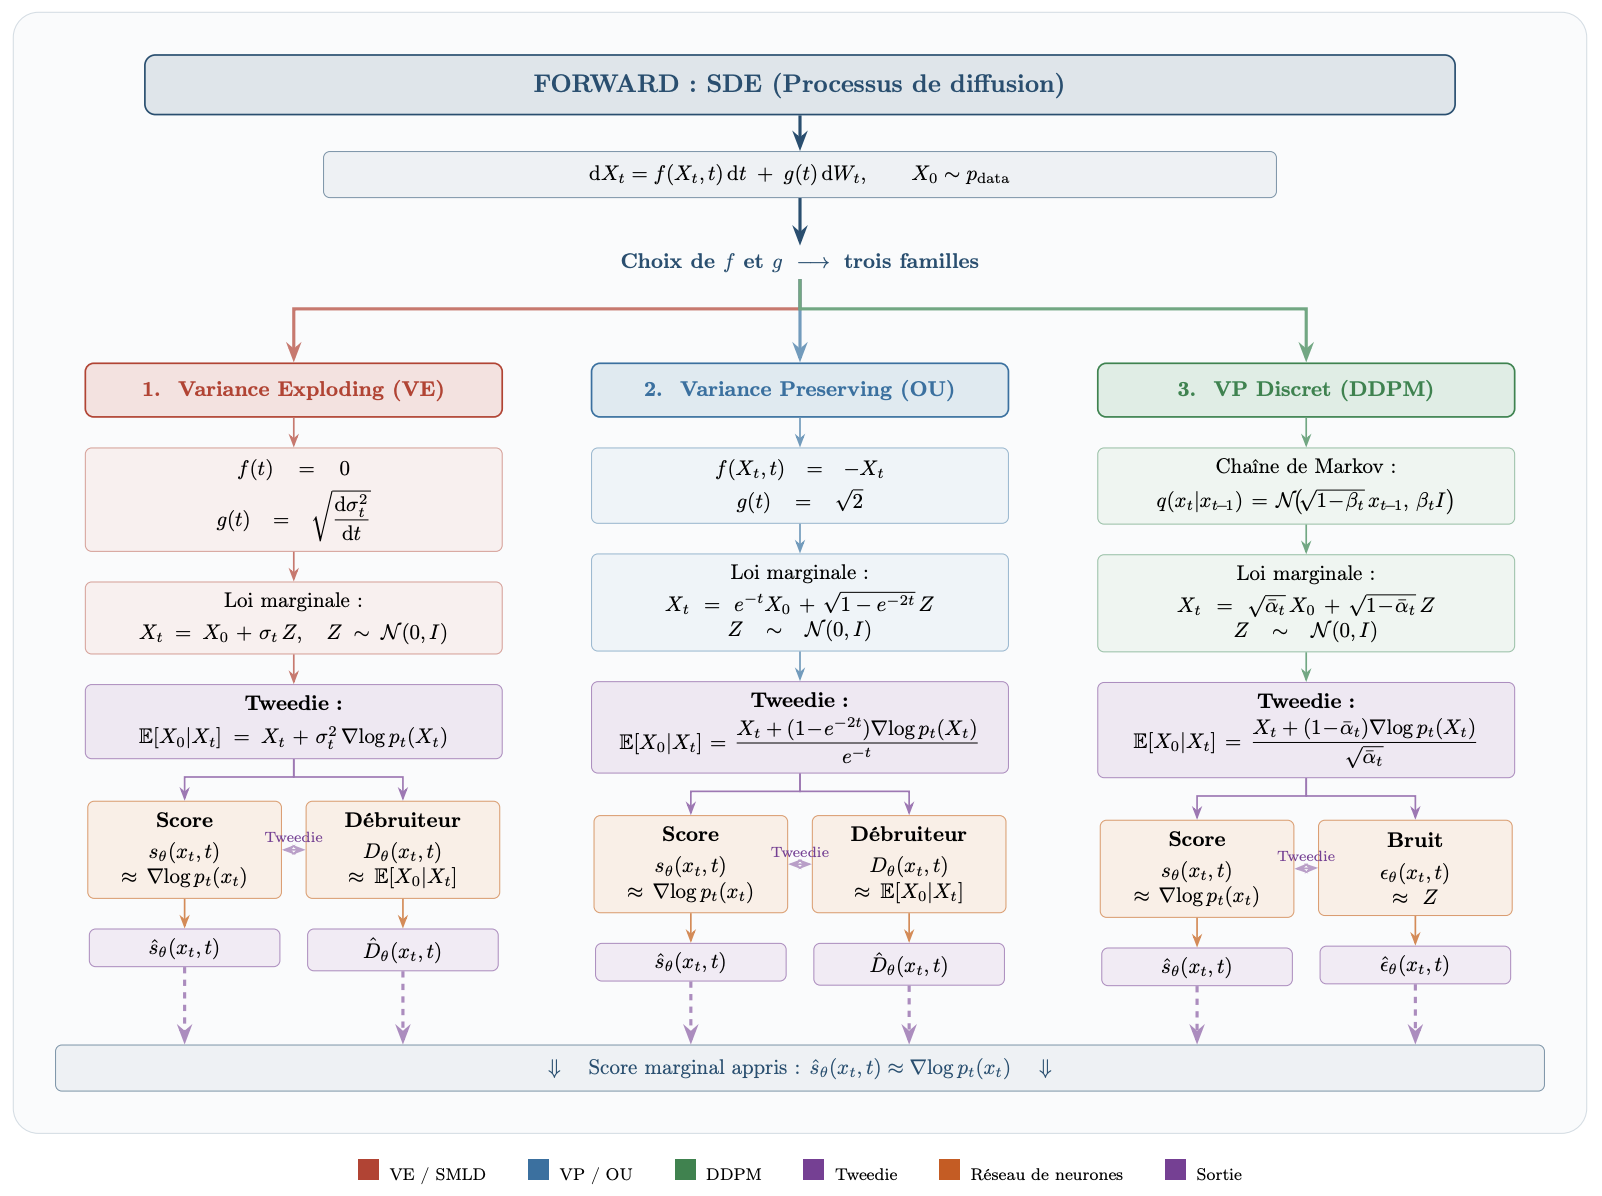
\includegraphics[width=\textwidth]{figure/Schema_Forward_MD.png}
\caption{Pipeline forward : de la SDE aux trois variantes, avec le lien Tweedie entre score et denoiser.}
\label{fig:forward}
\end{figure}


\section{Génération d'images}

\subsection{SDE reverse}

\begin{theorembox}[Anderson, 1982 (admis \cite{anderson1982reverse})]
\label{thm:anderson}
Toute SDE forward (Définition \ref{def:sde}) admet une SDE reverse :
\begin{equation}
    \boxed{\mathrm{d}X_t = \left[f(X_t, t) - g(t)^2\, \nabla_{X_t} \log p_t(X_t)\right] \mathrm{d}t + g(t)\,\mathrm{d}\bar{W}_t}
    \label{eq:reverse_sde}
\end{equation}
\end{theorembox}

Le terme $-g^2 \nabla \log p_t$ pousse $X_t$ vers les régions de haute densité. L'algorithme : $X_T \sim \mathcal{N}(0,I)$, discrétiser de $T$ à $0$ en remplaçant le score par $s_\theta$ (Théorème \ref{thm:dsm}).

\subsection{DDPM vs DDIM}

\textbf{DDPM} : discrétisation stochastique, $T = 1000$ pas :
\[
x_{t-1} = \frac{1}{\sqrt{\alpha_t}}\!\left(x_t - \frac{1-\alpha_t}{\sqrt{1-\bar\alpha_t}}\,\epsilon_\theta\right) + \sigma_t z, \quad z \sim \mathcal{N}(0, I)
\]

\textbf{DDIM} : déterministe, 10--50 pas : $x_{t-1} = \sqrt{\bar\alpha_{t-1}}\, \hat{x}_0 + \sqrt{1-\bar\alpha_{t-1}}\, \epsilon_\theta$ où $\hat{x}_0$ est donné par le résultat \ref{thm:tweedie_vp}.

\subsection{Probability Flow ODE}

Équivalent déterministe (mêmes marginales) : $\mathrm{d}X_t = [f - \tfrac{1}{2}g^2 \nabla \log p_t]\,\mathrm{d}t$. DDIM en est une discrétisation. Le facteur $\frac{1}{2}$ compense l'absence du terme de bruit.

\section{Problèmes inverses}

Le processus reverse (Théorème \ref{thm:anderson}) permet de générer des images en intégrant la SDE inverse avec le score appris $s_\theta$. Pour résoudre un \textbf{problème inverse}, autrement dit, pour reconstruire $x_0$ à partir de mesures dégradées $y$, on remplace le score inconditionnel par le score conditionnel $\nabla \log p_t(x_t | y)$. 



\subsection{Formulation et exemples}

Dans de nombreuses applications en imagerie, on n'observe pas directement l'image $x_0$ mais une version dégradée $y$. Le modèle de diffusion, entraîné sur des images propres, fournit un a priori puissant pour reconstruire $x_0$ à partir de $y$.

\begin{definitionbox}[Problème inverse linéaire]
\label{def:inverse}
\begin{equation}
    y = Ax_0 + \sigma_b\, b, \qquad b \sim \mathcal{N}(0, I_m)
\end{equation}
où $A \in \mathbb{R}^{m \times n}$ est un opérateur linéaire connu et $\sigma_b > 0$ le niveau de bruit de mesure.
\end{definitionbox}

Ce formalisme couvre un large spectre de problèmes :
\begin{itemize}
    \item \textbf{Super-résolution} ($\times 4$) : $A$ est un sous-échantillonnage (moyennage de blocs $4 \times 4$). On observe une image basse résolution, on veut reconstruire les détails fins.
    \item \textbf{IRM accélérée} : $A = MF$ où $F$ est la transformée de Fourier 2D et $M$ un masque binaire qui ne retient que certaines fréquences. On observe un sous-ensemble des coefficients de Fourier.
    \item \textbf{Inpainting} : $A$ est un masque diagonal ($A_{ii} = 0$ pour les pixels manquants, $1$ sinon). On observe une image avec des régions occultées.
    \item \textbf{Défloutage} : $A$ est une convolution avec un noyau de flou (gaussien, mouvement). On observe une image floue.
\end{itemize}

On veut échantillonner l' \textbf{a posteriori} $p(x_0 | y)$ : l'ensemble des images naturelles compatibles avec les mesures $y$.


\subsection{Pourquoi échantillonner via la SDE reverse ?}

On dispose du score inconditionnel $\nabla \log p_t$ (via le denoiser entraîné, résultat \ref{thm:dsm}). L'idée est de guider la SDE reverse (Théorème \ref{thm:anderson}) par les mesures $y$ en remplaçant le score inconditionnel par le score conditionnel :
\begin{equation}
    \mathrm{d}\tilde{X}_t = \left[-f + g^2\, \nabla_x \log p_{T-t}(\tilde{X}_t \mid y)\right]\mathrm{d}t + g\,\mathrm{d}\bar{W}_t, \qquad \tilde{X}_0 \sim p_T(\cdot | y) \approx \mathcal{N}(0, I)
    \label{eq:cond_reverse}
\end{equation}
Par le même argument qu'Anderson, les marginales de ce processus sont $p_t(\cdot | y)$, et au temps final on obtient $p_0(\cdot | y) = p(x_0 | y)$.

Pourquoi ne pas faire du MCMC directement sur $p(x_0 | y)$ ? La SDE de diffusion offre un \textbf{schedule multiscale} naturel : à temps élevé (bruit fort), on résout les grandes structures ; à temps faible (bruit faible), on affine les détails. En pratique, quelques centaines de pas suffisent, contre des millions pour un MCMC naïf en dimension $n \approx 256 \times 256 \times 3 \approx 200\,000$.


\subsection{Décomposition du score conditionnel}

Par la règle de Bayes $p(x_t | y) \propto p_t(x_t)\, p(y | x_t)$, le score conditionnel se décompose :
\begin{equation}
    \boxed{\nabla_{x_t} \log p(x_t|y) = \underbrace{\nabla_{x_t} \log p_t(x_t)}_{\text{score a priori } (s_\theta)} + \underbrace{\nabla_{x_t} \log p(y|x_t)}_{\text{score likelihood}}}
    \label{eq:score_decomp}
\end{equation}

Le premier terme est connu : c'est le score appris par le denoiser (résultat \ref{thm:dsm}). Le second est intractable.


\subsection{Intractabilité du score de mesure}

\begin{propositionbox}[Forme du score de mesure]
\label{prop:intract}
\begin{equation}
    p(y | x_t) = \int p(y | x_0)\, \underbrace{p(x_0 | x_t)}_{\text{impossible à calculer}}\, \mathrm{d}x_0
\end{equation}
\end{propositionbox}

  \begin{proof}







\textbf{Étape 1 : marginalisation.} $p(y | x_t) = \int p(y, x_0 | x_t)\, \mathrm{d}x_0 = \int p(y | x_0, x_t)\, p(x_0 | x_t)\, \mathrm{d}x_0$.

\textbf{Étape 2 : structure de Markov.} $Y$ ne dépend de $X_t$ qu'à travers $X_0$ (chaîne $Y \leftarrow X_0 \to X_t$), donc $p(y | x_0, x_t) = p(y | x_0)$.

\textbf{Étape 3 : conclusion.} $p(y | x_t) = \int p(y | x_0)\, p(x_0 | x_t)\, \mathrm{d}x_0$.
\end{proof}

Le terme $p(y | x_0) = \mathcal{N}(y; Ax_0, \sigma_b^2 I)$ est connu. Mais $p(x_0 | x_t)$ est l'\textbf{a posteriori de débruitage} : par Bayes, $p(x_0 | x_t) \propto p(x_t | x_0)\, p_{\text{data}}(x_0)$, et l'a priori $p_{\text{data}}$ (distribution des images naturelles) est un objet complexe, multimodal, en dimension $n \approx 200\,000$. L'intégrale est impossible à calculer.

Le résultat \ref{thm:mmse} ne donne que $\mathbb{E}[X_0 | X_t]$ (la moyenne), pas la distribution entière $p(x_0 | x_t)$. Toutes les méthodes ci-dessous approximent $p(x_0 | x_t)$ par une distribution simple. Dans ce compte rendu, nous ne détaillerons que DPS et $\Pi$GDM, mais la figure \ref{fig:reverse} propose un panorama un peu plus large des approches possibles.

\begin{remarkbox}[Tweedie conditionnel]
En appliquant Tweedie à la loi conditionnelle $p_t(\cdot | y)$ au lieu de $p_t$, on a:
\[
\mathbb{E}[X_0 | X_t, Y = y] = \underbrace{\mathbb{E}[X_0 | X_t]}_{\hat{x}_0 \;\text{(denoiser)}} + \sigma_t^2\, \nabla_{x_t} \log p(y | x_t)
\]
\end{remarkbox}


\subsection{DPS : approximation Dirac}

Chung et al.\ (2023) posent l'approximation la plus brutale : $p(x_0 | x_t) \approx \delta(x_0 - \hat{x}_0)$, où $\hat{x}_0 = \mathbb{E}[X_0 | X_t]$ est le denoiser de Tweedie.

\begin{resultbox}[DPS --- Diffusion Posterior Sampling]
\label{res:dps}
\begin{equation}
    \nabla_{x_t} \log p(y | x_t) \approx \nabla_{x_t} \log p(y | \hat{x}_0)
\end{equation}
\end{resultbox}

  \begin{proof}







\textbf{Étape 1 : approximation Dirac.} En substituant $p(x_0 | x_t) \approx \delta(x_0 - \hat{x}_0)$ dans la Proposition \ref{prop:intract} :
\[
p(y | x_t) \approx \int p(y | x_0)\, \delta(x_0 - \hat{x}_0)\, \mathrm{d}x_0 = p(y | \hat{x}_0)
\]

\textbf{Étape 2 : gradient.} $\hat{x}_0 = \hat{x}_0(x_t)$ dépend de $x_t$ via Tweedie. Par la règle de la chaîne :
\[
\nabla_{x_t} \log p(y | \hat{x}_0) = \left(\frac{\partial \hat{x}_0}{\partial x_t}\right)^{\!T} \nabla_{\hat{x}_0} \log p(y | \hat{x}_0)
\]

\textbf{Étape 3 : cas linéaire.} Pour $y = Ax_0 + \sigma_b b$, $p(y | \hat{x}_0) = \mathcal{N}(y; A\hat{x}_0, \sigma_b^2 I)$ :
\[
\nabla_{x_t} \log p(y | \hat{x}_0) = \frac{1}{\sigma_b^2}\left(\frac{\partial \hat{x}_0}{\partial x_t}\right)^{\!T} A^T(y - A\hat{x}_0)
\]
Par Tweedie, $\hat{x}_0 = x_t + \sigma_t^2 \nabla \log p_t(x_t)$, donc $\frac{\partial \hat{x}_0}{\partial x_t} = I_n + \sigma_t^2\, \nabla_{x_t}^2 \log p_t(x_t)$.

\textbf{Étape 4 : limitation.} L'approximation Dirac ignore toute l'incertitude de $p(x_0 | x_t)$ : quand $t$ est grand ($\sigma_t$ grand), $\hat{x}_0$ est un estimateur très bruité de $X_0$, et concentrer toute la masse en ce point est une approximation grossière.
\end{proof}


\subsection{$\Pi$GDM : approximation gaussienne}

Song et al.\ (2023) améliorent DPS en modélisant l'incertitude du denoiser.

\begin{hypothesebox}[$\Pi$GDM --- Song et al., 2023]
\label{hyp:pigdm}
\begin{enumerate}[label=(H\arabic*)]
    \item $p(x_0 | x_t) \approx \mathcal{N}(\hat{x}_0,\; r_t^2 I_n)$ \quad (gaussienne isotrope de rayon $r_t$)
    \item $y = Ax_0 + \sigma_b b$ \quad (Définition \ref{def:inverse})
\end{enumerate}
\end{hypothesebox}

Le paramètre $r_t^2$ capture l'incertitude du denoiser : grand quand $t$ est grand (beaucoup de bruit, $\hat{x}_0$ imprécis), petit quand $t \to 0$ (peu de bruit, $\hat{x}_0 \to x_0$).

\begin{resultbox}[Vraisemblance $\Pi$GDM]
\label{res:pigdm}
\begin{equation}
    p(y | x_t) \approx \mathcal{N}\!\left(A\hat{x}_0,\; \Sigma_y\right), \qquad \Sigma_y = \sigma_b^2 I_m + r_t^2\, AA^T
\end{equation}
\end{resultbox}

  \begin{proof}







\textbf{Étape 1 : modèle conditionnel.} Sous (H1) : $x_0 | x_t \sim \mathcal{N}(\hat{x}_0, r_t^2 I_n)$. Sous (H2) : $y | x_0 \sim \mathcal{N}(Ax_0, \sigma_b^2 I_m)$.

\textbf{Étape 2 : espérance de $y | x_t$.} Par la tour : $\mathbb{E}[y|x_t] = \mathbb{E}[\mathbb{E}[y|x_0] | x_t] = \mathbb{E}[Ax_0 | x_t] = A\hat{x}_0$.

\textbf{Étape 3 : variance de $y | x_t$.} Par la loi de la variance totale :
\begin{align}
    \mathrm{Var}(y|x_t) &= \underbrace{\mathrm{Var}(\mathbb{E}[y|x_0] | x_t)}_{= \mathrm{Var}(Ax_0 | x_t) = A(r_t^2 I)A^T} + \underbrace{\mathbb{E}[\mathrm{Var}(y|x_0) | x_t]}_{= \sigma_b^2 I_m} = r_t^2 AA^T + \sigma_b^2 I_m \nonumber
\end{align}

\textbf{Étape 4 : loi résultante.} $y | x_t$ est une transformation affine de gaussiennes (sous les hypothèses), donc gaussien : $y | x_t \sim \mathcal{N}(A\hat{x}_0, \Sigma_y)$.

\textbf{Étape 5 : gradient.} Par la règle de la chaîne ($x_t \to \hat{x}_0(x_t) \to \log p$) :
\[
\nabla_{x_t} \log p(y|x_t) = \left(\frac{\partial \hat{x}_0}{\partial x_t}\right)^{\!T} A^T \Sigma_y^{-1}(y - A\hat{x}_0)
\]



\textbf{Étape 6 : inversion par Woodbury.} Pour éviter d'inverser $\Sigma_y \in \mathbb{R}^{m \times m}$ :
\[
(\sigma_b^2 I + r_t^2 AA^T)^{-1} = \frac{1}{\sigma_b^2}\!\left(I - \frac{r_t^2}{\sigma_b^2}\, A\!\left(I + \frac{r_t^2}{\sigma_b^2}\, A^T A\right)^{\!-1}\!\! A^T\right)
\]
ce qui ramène à l'inversion d'une matrice $n \times n$ au lieu de $m \times m$ (ce qui reste tout de même embêtant, car il reste toujours à inverser une matrice).
\end{proof}

\subsection{Synthèse de processus reverse}
\vspace*{-0.7cm}
\begin{figure}[h!]
\centering
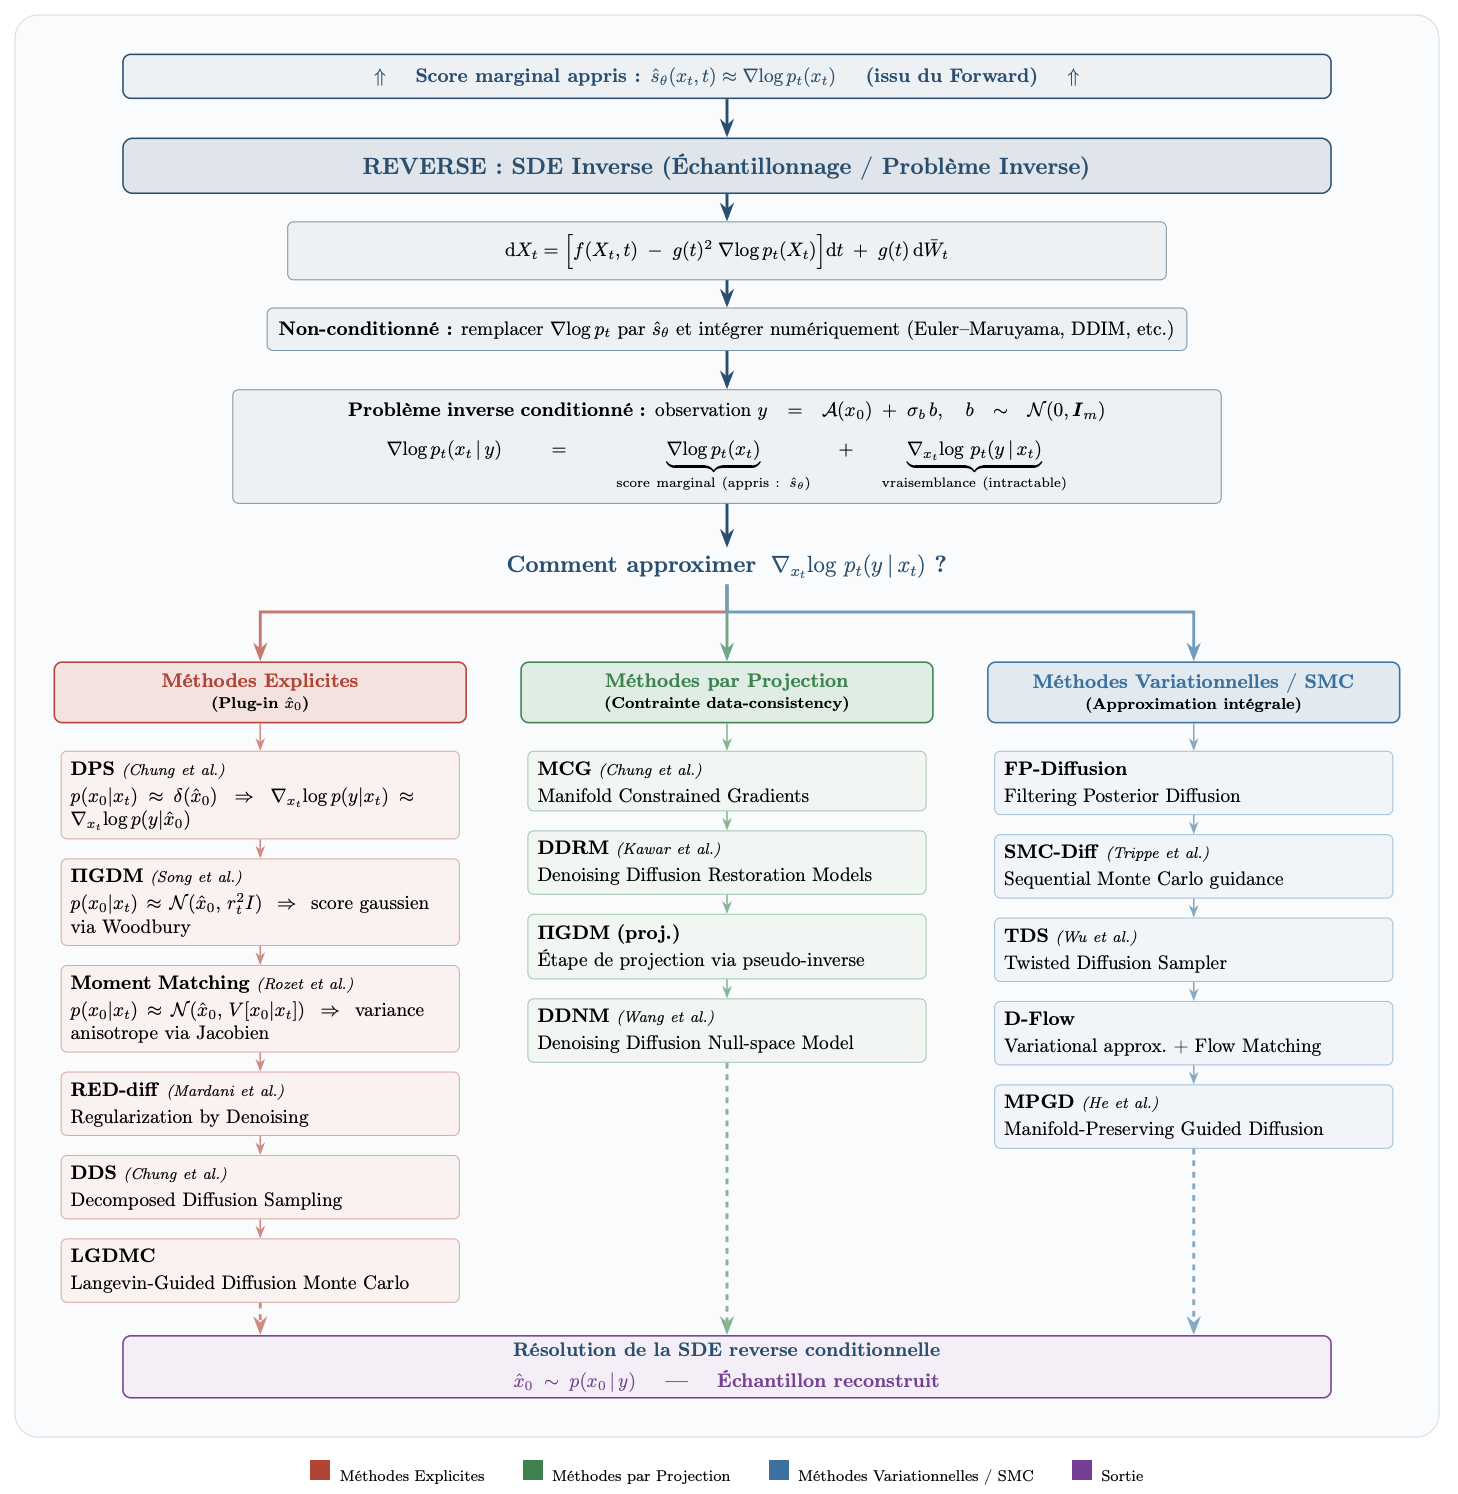
\includegraphics[width=0.97\textwidth]{figure/Schema_Reverse_MD.png}
\caption{Pipeline reverse conditionnée : décomposition du score conditionnel et les trois familles de méthodes d'approximation}
\label{fig:reverse}
\end{figure}


\newpage

\part{Tentative d'une nouvelle approche}

\section{Motivation}

La partie I a montré que certaines méthodes de résolution de problèmes inverses par diffusion (DPS et $\Pi$GDM) partagent une difficulté commune : elles dépendent d'hyperparamètres ($r_t^2$, $\sigma_b^2$, step size) fixés manuellement. En pratique, un mauvais réglage dégrade significativement la reconstruction.

L'idée de cette partie est de repartir du cadre $\Pi$GDM (Résultat \ref{res:pigdm}) et d'exprimer le score conditionnel $\nabla_{x_t} \log p_t(x_t | y)$ sous forme explicite, ce qui permettra potentiellement ensuite d'optimiser $r_t^2$ et $\sigma_b^2$ par inférence variationnelle au lieu de les fixer à la main.


\section{Rappels et hypothèses}

On se place dans le cadre VP-DDPM (Résultat \ref{res:ddpm}) pour fixer les notations.

\begin{rappelbox}[Loi marginale forward (VP-DDPM)]
\begin{equation}
    X_t = \sqrt{\bar\alpha_t}\, X_0 + \sqrt{1-\bar\alpha_t}\, Z, \qquad Z \sim \mathcal{N}(0, I_n)
    \label{eq:vp_recall}
\end{equation}
En particulier : $X_t | X_0 \sim \mathcal{N}\!\left(\sqrt{\bar\alpha_t}\, X_0,\; (1-\bar\alpha_t)\, I_n\right)$.
\end{rappelbox}

\begin{rappelbox}[Tweedie conditionnel (VP-DDPM)]
Le score de la marginale $p_t$ et celui de la conditionnelle $p_t(\cdot | x_0)$ s'écrivent :
\begin{align}
    \nabla_{x_t} \log p_t(x_t | x_0) &= \frac{\sqrt{\bar\alpha_t}\, x_0 - x_t}{1 - \bar\alpha_t} \label{eq:score_cond}\\[6pt]
    \nabla_{x_t} \log p_t(x_t) &= \frac{\sqrt{\bar\alpha_t}\, \mathbb{E}[X_0 | X_t = x_t] - x_t}{1 - \bar\alpha_t} \label{eq:score_marg}
\end{align}
On note $\hat{x}_0(x_t) = \mathbb{E}[X_0 | X_t = x_t]$ le denoiser de Tweedie, approché par le réseau $s_\theta$.
\end{rappelbox}

\begin{hypothesebox}[$\Pi$GDM --- approximation gaussienne isotrope]
\label{hyp:pigdm2}
\begin{equation}
    X_0 \mid X_t = x_t \;\sim\; \mathcal{N}\!\left(\hat{x}_0(x_t),\; r_t^2\, I_n\right)
    \tag{H1}
    \label{eq:H1}
\end{equation}
\end{hypothesebox}

\begin{hypothesebox}[Problème inverse linéaire gaussien]
\label{hyp:linear2}
\begin{equation}
    y = A\, x_0 + b, \qquad b \sim \mathcal{N}(0,\, \sigma_b^2\, I_m)
    \tag{H2}
    \label{eq:H2}
\end{equation}
\end{hypothesebox}

Ces deux hypothèses impliquent la structure de dépendance suivante :
\begin{rappelbox}[Dépendances]
\begin{enumerate}[label=(D\arabic*)]
    \item $y = f(x_0, \sigma_b^2)$ \quad (par \ref{eq:H2})
    \item $x_0 \sim g(x_t, r_t^2)$ \quad (par \ref{eq:H1})
    \item $x_t = h(x_0, \bar\alpha_t)$ \quad (par \eqref{eq:vp_recall})
\end{enumerate}
En particulier, la chaîne de Markov $Y \leftarrow X_0 \to X_t$ implique $Y \indep X_t \mid X_0$ : les mesures $y$ ne dépendent pas directement de $x_t$, seulement à travers $x_0$.
\end{rappelbox}


\section{Score conditionnel en forme fermée}

L'objectif est d'exprimer $\nabla_{x_t} \log p_t(x_t | y)$ de manière exploitable algorithmiquement.

\subsection{Étape 1 : Tweedie conditionnel appliqué à $p_t(\cdot | y)$}

\begin{propositionbox}[Score conditionnel via Tweedie]
\label{prop:score_cond_y}
En appliquant la formule de Tweedie à la distribution conditionnelle $p_t(\cdot | y)$ :
\begin{equation}
    \boxed{\nabla_{x_t} \log p_t(x_t | y) = \frac{\sqrt{\bar\alpha_t}\, \mathbb{E}[X_0 | X_t = x_t,\, Y = y] - x_t}{1 - \bar\alpha_t}}
    \label{eq:score_cond_y}
\end{equation}
\end{propositionbox}

 \begin{proof}







\textbf{Étape 1 : marginalisation.}
\[
p_t(x_t | y) = \int p_t(x_t, x_0 | y)\, \mathrm{d}x_0 = \int \frac{p(y | x_0)\, p_t(x_t | x_0)\, p(x_0)}{p(y)}\, \mathrm{d}x_0
\]
où l'on a utilisé $p(y | x_0, x_t) = p(y | x_0)$ (chaîne de Markov $Y \leftarrow X_0 \to X_t$) et la décomposition $p_t(x_t, x_0) = p_t(x_t | x_0)\, p(x_0)$ (D1).\\

\textbf{Étape 2 : gradient.} \\
En dérivant sous l'intégrale par rapport à $x_t$, seul le terme $p_t(x_t | x_0)$ dépend de $x_t$ :
\[
\nabla_{x_t} p_t(x_t | y) = \int \text{cte} \cdot p(y | x_0) \cdot \nabla_{x_t} p_t(x_t | x_0) \cdot p(x_0)\, \mathrm{d}x_0
\]
Or, \[\nabla_{x_t} \log p_t(x_t | x_0)=\frac{\nabla_{x_t} p_t(x_t | x_0)}{ p_t(x_t | x_0)}\] 
Et par \eqref{eq:score_cond} : 
\[\nabla_{x_t} p_t(x_t | x_0) = p_t(x_t | x_0) \cdot \frac{\sqrt{\bar\alpha_t}\, x_0 - x_t}{1 - \bar\alpha_t}\] 

Donc :
\[
\nabla_{x_t} p_t(x_t | y) = \int \text{cte} \cdot p(y | x_0) \cdot p_t(x_t | x_0) \cdot p(x_0) \cdot \frac{\sqrt{\bar\alpha_t}\, x_0 - x_t}{1 - \bar\alpha_t}\, \mathrm{d}x_0
\]

\textbf{Étape 3 : identification de l'a posteriori jointe.}\\
 On reconnaît :
\[
p_t(x_0 | x_t, y) = \frac{p(y | x_0)\, p_t(x_t | x_0)\, p(x_0)}{p_t(x_t | y)\, p(y)}
\]
En divisant le numérateur et le dénominateur par $p_t(x_t | y)$ :
\[
\nabla_{x_t} \log p_t(x_t | y) = \frac{\nabla_{x_t} p_t(x_t | y)}{p_t(x_t | y)} = \int p_t(x_0 | x_t, y) \cdot \frac{\sqrt{\bar\alpha_t}\, x_0 - x_t}{1 - \bar\alpha_t}\, \mathrm{d}x_0 = \frac{\sqrt{\bar\alpha_t}\, \mathbb{E}[X_0 | x_t, y] - x_t}{1 - \bar\alpha_t}
\]
\end{proof}

Il reste donc à calculer $\mathbb{E}[X_0 | X_t, Y]$ de manière explicite.


\subsection{Étape 2 : loi de $X_0 | X_t, Y$ sous les hypothèses $\Pi$GDM}

\begin{propositionbox}[A posteriori jointe]
\label{prop:posterior_joint}
Sous \ref{eq:H1} et \ref{eq:H2} :
\begin{equation}
    p_t(x_0 \mid x_t, y) \;\propto\; p(y \mid x_0) \cdot p_t(x_0 \mid x_t)
    \label{eq:posterior_prop}
\end{equation}
\end{propositionbox}

 \begin{proof}






\textbf{Étape 1 : Bayes.} Par la règle de Bayes :
\[
p_t(x_0 \mid x_t, y) = \frac{p(y \mid x_0, x_t)\, p_t(x_0 \mid x_t)}{p_t(y \mid x_t)}
\]

\textbf{Étape 2 : Markov.} Par la chaîne $Y \leftarrow X_0 \to X_t$ , on a $p(y \mid x_0, x_t) = p(y \mid x_0)$ (D1).

\textbf{Étape 3 : conclusion.} Le dénominateur $p_t(y \mid x_t)$ est indépendant de $x_0$, donc :
\[
p_t(x_0 \mid x_t, y) \propto p(y \mid x_0) \cdot p_t(x_0 \mid x_t)
\]
\end{proof}


\subsection{Étape 3 : produit de gaussiennes et complétion du carré}

Sous nos hypothèses, les deux termes du produit sont gaussiens :
\begin{align}
    p(y \mid x_0) &= \mathcal{N}(y;\; Ax_0,\; \sigma_b^2 I_m) \quad \text{(par \ref{eq:H2})} \\
    p_t(x_0 \mid x_t) &= \mathcal{N}(x_0;\; \hat{x}_0(x_t),\; r_t^2 I_n) \quad \text{(par \ref{eq:H1})}
\end{align}

\begin{resultbox}[A posteriori gaussienne en forme fermée]
\label{thm:posterior_closed}
Sous \ref{eq:H1} et \ref{eq:H2}, l'a posteriori $p_t(x_0 \mid x_t, y)$ est gaussienne :
\begin{equation}
    X_0 \mid X_t, Y \;\sim\; \mathcal{N}(\mu_{\text{post}},\; \Sigma_{\text{post}})
\end{equation}
avec :
\begin{equation}
    \boxed{\Sigma_{\text{post}} = \left(\frac{A^T A}{\sigma_b^2} + \frac{I_n}{r_t^2}\right)^{\!-1}}
    \label{eq:sigma_post}
\end{equation}
\begin{equation}
    \boxed{\mu_{\text{post}} = \Sigma_{\text{post}} \left(\frac{A^T y}{\sigma_b^2} + \frac{\hat{x}_0(x_t)}{r_t^2}\right)}
    \label{eq:mu_post}
\end{equation}
\end{resultbox}

 \begin{proof}



\textbf{Étape 1 : log-a posteriori.} Par la Proposition \ref{prop:posterior_joint} et les hypothèses \ref{eq:H1} et \ref{eq:H2}:
\begin{align}
    \log p_t(x_0 \mid x_t, y) &= \log p(y \mid x_0) + \log p_t(x_0 \mid x_t) + \text{cte} \nonumber\\
    &= -\frac{\|y - Ax_0\|^2}{2\sigma_b^2} - \frac{\|x_0 - \hat{x}_0\|^2}{2r_t^2} + \text{cte} \label{eq:log_post}
\end{align}

\textbf{Étape 2 : développement et regroupement des termes en $x_0$.}
\begin{align}
    &= -\frac{1}{2}\left[x_0^T\!\left(\frac{A^T A}{\sigma_b^2} + \frac{I_n}{r_t^2}\right)\!x_0 - 2\, x_0^T\!\left(\frac{A^T y}{\sigma_b^2} + \frac{\hat{x}_0}{r_t^2}\right)\right] + \text{cte}
\end{align}

\textbf{Étape 3 : identification.} La forme quadratique $-\frac{1}{2}(x - \mu)^T \Sigma^{-1}(x - \mu)$ se développe en $-\frac{1}{2}[x^T \Sigma^{-1} x - 2x^T \Sigma^{-1}\mu] + \text{cte}$. Par identification :
\[
\Sigma_{\text{post}}^{-1} = \frac{A^T A}{\sigma_b^2} + \frac{I_n}{r_t^2}, \qquad \Sigma_{\text{post}}^{-1} \mu_{\text{post}} = \frac{A^T y}{\sigma_b^2} + \frac{\hat{x}_0}{r_t^2}
\]
En multipliant à gauche par $\Sigma_{\text{post}}$, on obtient les expressions annoncées.
\end{proof}

\begin{remarkbox}[Interprétation de $\mu_{\text{post}}$]
La moyenne a posteriori $\mu_{\text{post}}$ est un \textbf{compromis pondéré} entre deux sources d'information :
\begin{enumerate}[label=(\roman*)]
    \item le terme $\frac{A^T y}{\sigma_b^2}$, qui pousse vers la cohérence avec les mesures $y$, pondéré inversement par le bruit de mesure $\sigma_b^2$ ;
    \item le terme $\frac{\hat{x}_0}{r_t^2}$, qui pousse vers la prédiction du denoiser, pondéré inversement par l'incertitude du denoiser $r_t^2$.
\end{enumerate}
Quand $\sigma_b \to 0$ (mesures parfaites), $\mu_{\text{post}} \to A^\dagger y$ ; quand $r_t \to 0$ (denoiser parfait), $\mu_{\text{post}} \to \hat{x}_0$.
\end{remarkbox}


\subsection{Résultat principal : score conditionnel explicite}

En combinant la Proposition \ref{prop:score_cond_y} et le résultat \ref{thm:posterior_closed} :

\begin{resultbox}[Score conditionnel]
\label{res:score_vbpigdm}
Sous les hypothèses \ref{eq:H1}--\ref{eq:H2} :
\begin{equation}
    \boxed{\nabla_{x_t} \log p_t(x_t | y) = \frac{\sqrt{\bar\alpha_t}\;\mu_{\text{post}} - x_t}{1 - \bar\alpha_t}}
    \label{eq:score_vbpigdm}
\end{equation}
où :
\[
\mu_{\text{post}} = \left(\frac{A^T A}{\sigma_b^2} + \frac{I_n}{r_t^2}\right)^{\!-1} \left(\frac{A^T y}{\sigma_b^2} + \frac{\hat{x}_0(x_t)}{r_t^2}\right)
\]
et $\hat{x}_0(x_t) = \mathbb{E}[X_0 | X_t = x_t]$ est le denoiser de Tweedie approché par $s_\theta$.
\end{resultbox}

\begin{remarkbox}[Lien avec DPS et $\Pi$GDM classique]
On retrouve les méthodes précédentes comme cas limites :
\begin{enumerate}[label=(\roman*)]
    \item $r_t^2 \to 0$ : $\mu_{\text{post}} \to \hat{x}_0$, et on retrouve le score DPS.
    \item $\Pi$GDM classique (Résultat \ref{res:pigdm}) calcule $\nabla_{x_t} \log p(y | x_t)$ séparément, puis l'ajoute au score inconditionnel. Ici, on obtient directement le score conditionnel total, ce qui évite les problèmes numériques liés à la somme de deux termes de grandeurs très différentes.
\end{enumerate}
\end{remarkbox}

\subsection{Vers l'optimisation variationnelle de $r_t^2$ et $\sigma_b^2$}

Le Résultat 
\ref{res:score_vbpigdm} fournit le score conditionnel en forme fermée, mais dépend de deux hyperparamètres fixés manuellement 
: $r_t^2$ (incertitude du denoiser) et $\sigma_b^2$ (bruit de mesure). L'idée est de les traiter comme des \textbf{variables latentes} et de les estimer automatiquement par inférence variationnelle bayésienne (VB).

\newpage

\section{Modèle hiérarchique bayésien}

\subsection{Variables et structure}

On reformule le problème en distinguant les quantités observées des quantités à inférer.

\begin{definitionbox}[Variables du modèle]
\label{def:vb_variables}
\textbf{Observations} 
: $\boldsymbol{y} = (x_t,\, y,\, \hat{x}_0(x_t),\, A)$.

\textbf{Variables latentes} 
: $\boldsymbol{w} = (x_0,\, \tau_r,\, \tau_b)$, où 
:
\begin{align}
    \tau_r &= 1/r_t^2 \quad \text{(précision du denoiser)} \\
    \tau_b &= 1/\sigma_b^2 \quad \text{(précision du bruit de mesure)}
\end{align}
On paramétrise en précisions $\tau$ plutôt qu'en variances $\sigma^2$ car les lois conjuguées (Gamma) s'expriment naturellement en précision.
\end{definitionbox}


\subsection{Lois du modèle génératif}

\begin{hypothesebox}[Modèle hiérarchique VB + $\Pi$GDM]
\label{hyp:hierarchical}
\begin{align}
    x_t \mid x_0 &\sim \mathcal{N}\!\left(\sqrt{\bar\alpha_t}\, x_0,\; (1 - \bar\alpha_t)\, I_n\right) \tag{M1} \label{eq:M1}\\[4pt]
    x_0 \mid \tau_r &\sim \mathcal{N}\!\left(\hat{x}_0(x_t),\; \tau_r^{-1}\, I_n\right) \tag{M2} \label{eq:M2}\\[4pt]
    y \mid x_0,\, \tau_b &\sim \mathcal{N}\!\left(A\, x_0,\; \tau_b^{-1}\, I_m\right) \tag{M3} \label{eq:M3}\\[4pt]
    \tau_r &\sim \mathrm{Gamma}(a_0,\, b_0) \tag{M4} \label{eq:M4}\\[4pt]
    \tau_b &\sim \mathrm{Gamma}(c_0,\, d_0) \tag{M5} \label{eq:M5}
\end{align}
\end{hypothesebox}

Les équations \ref{eq:M1}--\ref{eq:M3} reprennent exactement les hypothèses de la partie précédente (SDE forward, $\Pi$GDM, problème inverse linéaire), et \ref{eq:M4}--\ref{eq:M5} ajoutent des a prioris conjugués sur les précisions.

\begin{remarkbox}[Indépendances conditionnelles]
La structure du modèle implique 
:
\begin{enumerate}[label=(\roman*)]
    \item $\tau_r \indep \tau_b$ \quad (a prioris indépendants)
    \item $x_t \indep y \mid x_0$ \quad (chaîne de Markov $x_t \leftarrow x_0 \to y$)
    \item $x_t \indep \tau_b \mid x_0$ \quad (le forward ne dépend pas du bruit de mesure)
    \item $y \indep \tau_r \mid x_0$ \quad (les mesures ne dépendent pas de l'incertitude du denoiser)
\end{enumerate}
\end{remarkbox}


\subsection{Loi jointe}

\begin{propositionbox}[Factorisation de la loi jointe]
\label{prop:joint}
\begin{equation}
    \boxed{p_t(\boldsymbol{w}, \boldsymbol{y}) = p_t(x_t \mid x_0) \cdot p(y \mid x_0, \tau_b) \cdot p(x_0 \mid \tau_r) \cdot p(\tau_r) \cdot p(\tau_b)}
    \label{eq:joint}
\end{equation}
\end{propositionbox}

 \begin{proof}





Par la règle de la chaîne et les indépendances conditionnelles 
:
\begin{align}
    p_t(x_0, x_t, y, \tau_r, \tau_b) &= p_t(x_t \mid x_0, y, \tau_r, \tau_b) \cdot p(y \mid x_0, \tau_r, \tau_b) \cdot p(x_0 \mid \tau_r, \tau_b) \cdot p(\tau_r, \tau_b) \nonumber\\
    &= p_t(x_t \mid x_0) \cdot p(y \mid x_0, \tau_b) \cdot p(x_0 \mid \tau_r) \cdot p(\tau_r) \cdot p(\tau_b)
\end{align}
où l'on a utilisé 
: $x_t \indep (y, \tau_r, \tau_b) \mid x_0$, puis $y \indep \tau_r \mid x_0$, puis $x_0 \indep \tau_b \mid \tau_r$, et enfin $\tau_r \indep \tau_b$.
\end{proof}


\subsection{Log-vraisemblance jointe}

On calcule $\log p_t(\boldsymbol{w}, \boldsymbol{y})$ terme par terme.

\begin{propositionbox}[Termes de la log-jointe]
\label{prop:logterms}
En ne gardant que les termes qui dépendent de $\boldsymbol{w} = (x_0, \tau_r, \tau_b)$ 
:

\textbf{Terme 1 
:} par \ref{eq:M1}, $x_t \mid x_0 \sim \mathcal{N}(\sqrt{\bar\alpha_t}\, x_0,\, (1-\bar\alpha_t)\, I_n)$ 
:
\begin{equation}
    \log p_t(x_t \mid x_0) = -\frac{1}{2(1-\bar\alpha_t)} \|x_t - \sqrt{\bar\alpha_t}\, x_0\|^2 + \mathrm{cte}
\end{equation}

\textbf{Terme 2 
:} par \ref{eq:M3}, $y \mid x_0, \tau_b \sim \mathcal{N}(Ax_0,\, \tau_b^{-1} I_m)$ 
:
\begin{equation}
    \log p(y \mid x_0, \tau_b) = \frac{m}{2}\log \tau_b - \frac{\tau_b}{2}\|y - Ax_0\|^2 + \mathrm{cte}
\end{equation}

\textbf{Terme 3 
:} par \ref{eq:M2}, $x_0 \mid \tau_r \sim \mathcal{N}(\hat{x}_0,\, \tau_r^{-1} I_n)$ 
:
\begin{equation}
    \log p(x_0 \mid \tau_r) = \frac{n}{2}\log \tau_r - \frac{\tau_r}{2}\|x_0 - \hat{x}_0\|^2 + \mathrm{cte}
\end{equation}

\textbf{Terme 4 
:} par \ref{eq:M4}, $\tau_r \sim \mathrm{Gamma}(a_0, b_0)$ 
:
\begin{equation}
    \log p(\tau_r) = (a_0 - 1)\log \tau_r - b_0\, \tau_r + \mathrm{cte}
\end{equation}

\textbf{Terme 5 
:} par \ref{eq:M5}, $\tau_b \sim \mathrm{Gamma}(c_0, d_0)$ 
:
\begin{equation}
    \log p(\tau_b) = (c_0 - 1)\log \tau_b - d_0\, \tau_b + \mathrm{cte}
\end{equation}
\end{propositionbox}

 \begin{proof}





Chaque terme s'obtient en développant la log-densité correspondante et en absorbant dans $\mathrm{cte}$ tout ce qui ne dépend pas de $(x_0, \tau_r, \tau_b)$.

Pour le terme 
1 
: $\log \mathcal{N}(x_t;\, \mu, \sigma^2 I) = -\frac{n}{2}\log(2\pi\sigma^2) - \frac{1}{2\sigma^2}\|x_t - \mu\|^2$. Le premier terme est indépendant de $x_0$, d'où le résultat.

Pour les termes 
2 et 
3 
: même développement, mais la précision $\tau = 1/\sigma^2$ apparaît comme facteur multiplicatif devant la norme et comme $\frac{n}{2}\log\tau$.

Pour les termes 
4 et 
5 
: la densité Gamma$(\alpha, \beta)$ est $p(\tau) \propto \tau^{\alpha-1} e^{-\beta\tau}$, d'où $\log p(\tau) = (\alpha-1)\log\tau - \beta\tau + \mathrm{cte}$.
\end{proof}

En sommant les cinq termes 
:

\begin{resultbox}[Log-vraisemblance jointe]
\label{res:logjoint}
\begin{equation}
    \boxed{\begin{aligned}
        \log p_t(\boldsymbol{w}, \boldsymbol{y}) \;=\;
        &-\frac{1}{2(1-\bar\alpha_t)}\|x_t - \sqrt{\bar\alpha_t}\, x_0\|^2 \\[4pt]
        &+ \left(\frac{m}{2} + c_0 - 1\right)\log\tau_b - \left(d_0 + \tfrac{1}{2}\|y - Ax_0\|^2\right)\tau_b \\[4pt]
        &+ \left(\frac{n}{2} + a_0 - 1\right)\log\tau_r - \left(b_0 + \tfrac{1}{2}\|x_0 - \hat{x}_0\|^2\right)\tau_r \\[4pt]
        &+ \;\mathrm{cte}
    \end{aligned}}
    \label{eq:logjoint}
\end{equation}
\end{resultbox}


\section{Approximation variationnelle}

\subsection{Pourquoi approcher l'a posteriori ?}

On dispose de la loi jointe $p_t(\w, \y)$ (Résultat 
\ref{res:logjoint}), mais l'objectif est d'échantillonner selon l'a posteriori $p_t(\w | \y)$. Or, par la règle de Bayes 
:
\[
p_t(\w | \y) = \frac{p_t(\w, \y)}{p_t(\y)}, \qquad \text{où} \quad p_t(\y) = \int p_t(\w, \y)\, \mathrm{d}\w
\]
L'intégrale de normalisation $p_t(\y)$ porte sur toutes les variables latentes $\w = (x_0, \tau_r, \tau_b)$ en dimension $n + 2$. En imagerie, $n \approx 200\,000$ : cette intégrale est intractable. Connaître la jointe ne suffit donc pas, il faut approcher l'a posteriori.

\subsection{Choix de la mesure de dissemblance}

On cherche une densité approchante $q(\w)$ la plus proche possible de $p_t(\w | \y)$. La ``proximité'' se mesure par une mesure de dissemblance $\Delta(q \| p_t(\cdot|\y))$. Un choix naturel est la divergence de Kullback-Leibler $\mathcal{KL}$, qui mesure la différence entre deux densités de probabilité :
\begin{equation}
    \mathcal{KL}[q \| p_t(\cdot|\y)] = \int_{\mathbb{R}^{n+2}} q(\w) \log \frac{q(\w)}{p_t(\w|\y)}\, \mathrm{d}\w
    \label{eq:kl_def}
\end{equation}

Cette divergence possède les propriétés suivantes :
\begin{itemize}
    \item $\mathcal{KL}[q \| p] \geq 0$ pour tout $q, p$, avec égalité si et seulement si $q = p$ presque partout ;
    \item elle est \textbf{asymétrique} : $\mathcal{KL}[q \| p] \neq \mathcal{KL}[p \| q]$ en général ;
    \item elle est convexe.
\end{itemize}

En raison de l'asymétrie de $\mathcal{KL}$, deux possibilités existent selon l'ordre des arguments :

\begin{enumerate}[label=(\roman*)]
    \item \textbf{Divergence $\mathcal{KL}_{RM}$} : $\mathcal{KL}[p_t(\cdot|\y) \| q]$. Cette divergence est optimale d'un point de vue bayésien car sa minimisation donne une approximation de risque minimale. Cependant, elle est inutilisable en pratique car elle nécessite de connaître les lois marginales $p_t(w_j | \y)$.
    
    \item \textbf{Divergence $\mathcal{KL}_{BV}$} : $\mathcal{KL}[q \| p_t(\cdot|\y)]$. Les méthodes d'approximation bayésienne variationnelle utilisent cette divergence car elle permet d'obtenir des solutions analytiques, comme on le verra dans la suite.
\end{enumerate}

En pratique, $\mathcal{KL}_{BV}$ n'est pas directement calculable car elle dépend de $p_t(\w|\y)$, que l'on ne connaît pas (la fonction de partition $p_t(\y) = \int p_t(\w, \y)\, \mathrm{d}\w$ est intractable). On développe donc :
\begin{align}
    \mathcal{KL}_{BV} &= \int q(\w) \log \frac{q(\w)}{p_t(\w|\y)}\, \mathrm{d}\w = \int q(\w) \log \frac{q(\w)\, p_t(\y)}{p_t(\w, \y)}\, \mathrm{d}\w \nonumber\\[4pt]
    &= \log p_t(\y) - \underbrace{\int q(\w) \log \frac{p_t(\w, \y)}{q(\w)}\, \mathrm{d}\w}_{=: \mathcal{F}(q)}
    \label{eq:kl_decomp}
\end{align}

La quantité $\mathcal{F}(q) = \mathbb{E}_q\!\left[\log \frac{p_t(\w, \y)}{q(\w)}\right]$ est l'\textbf{énergie libre négative}. Elle ne dépend que de la loi jointe $p_t(\w, \y)$, que l'on connaît explicitement (Résultat \ref{res:logjoint}). Comme $\mathcal{KL}_{BV} \geq 0$, on a $\mathcal{F}(q) \leq \log p_t(\y)$ : l'énergie libre est une borne inférieure de la log-évidence.

\begin{resultbox}[Objectif variationnel]
\label{res:elbo}
\begin{equation}
    \boxed{\min_q \;\mathcal{KL}_{BV} \;\Longleftrightarrow\; \max_q \;\mathcal{F}(q)}
    \label{eq:elbo_equiv}
\end{equation}
Avec : 
\begin{equation}
\mathcal{F}(q) = \int q(\w) \log \frac{p_t(\w, \y)}{q(\w)}\, \mathrm{d}\w = \mathbb{E}_q\!\left[\log \frac{p_t(\w, \y)}{q(\w)}\right]
\end{equation}
\end{resultbox}

\begin{remarkbox}[Interprétation]
À convergence de l'algorithme BV, $\mathcal{KL}_{BV} \approx 0$ et donc $\mathcal{F}(q) \approx \ln p_t(\y)$. L'énergie libre peut ainsi servir d'approximation de la log-évidence pour la sélection de modèle.
\end{remarkbox}



\subsection{Hypothèse de champ moyen}

\begin{hypothesebox}[Factorisation champ moyen]
\label{hyp:meanfield}
On suppose que la densité approchante factorise 
:
\begin{equation}
    q(\w) = \left(\prod_{i=1}^{n} q_i(x_{0,i})\right) \cdot q(\tau_r)\, q(\tau_b)
    \tag{MF}
    \label{eq:MF}
\end{equation}
où $x_{0,i}$ désigne la $i$-ème composante de $x_0 \in \mathbb{R}^n$.
\end{hypothesebox}

Cette hypothèse rend toutes les variables latentes mutuellement indépendantes sous $q$ : chaque pixel $x_{0,i}$ est indépendant des autres et des précisions $\tau_r, \tau_b$. C'est l'hypothèse la plus fine du cadre champ moyen, qui permettra d'obtenir des mises à jour analytiques pour chaque facteur.

\begin{hypothesebox}[Forme paramétrique de $q(x_0)$]
\label{hyp:q_x0}
On choisit une famille gaussienne pour chaque composante :
\begin{equation}
    q_i(x_{0,i}) = \mathcal{N}(x_{0,i} \mid \mu_i,\, \Sigma_i), \quad i = 1, \ldots, n
    \label{eq:q_x0i}
\end{equation}
où $(\mu_i, \Sigma_i)_{i=1,\ldots,n}$ sont les paramètres variationnels à optimiser.
\end{hypothesebox}


\begin{rappelbox}[Lois des précisions (Hypothèses \ref{hyp:hierarchical})]
Les a priori conjugués sur les précisions induisent des lois approchantes de même famille :
\begin{align}
    q(\tau_r) &= \mathrm{Gamma}(\tau_r \mid a_0,\, b_0) \label{eq:q_taur_rappel}\\[4pt]
    q(\tau_b) &= \mathrm{Gamma}(\tau_b \mid c_0,\, d_0) \label{eq:q_taub_rappel}
\end{align}
\end{rappelbox}

\begin{remarkbox}[Notation vectorielle]
On note $\boldsymbol{\mu} = (\mu_1, \ldots, \mu_n)^T \in \mathbb{R}^n$ et $\boldsymbol{\Sigma} = (\Sigma_1, \ldots, \Sigma_n)^T \in \mathbb{R}^n$ les vecteurs des moyennes et variances marginales. Attention : $\Sigma_i$ est un \textbf{scalaire} (la variance du pixel $i$), pas une matrice. L'hypothèse champ moyen force la matrice de covariance de $q(x_0)$ à être diagonale : $\mathrm{Cov}_q(x_0) = \mathrm{diag}(\Sigma_1, \ldots, \Sigma_n)$.
\end{remarkbox}

\section{Optimisation dans l'espace des mesures}

La section précédente a réduit le problème à la maximisation de $\mathcal{F}(q) = \mathbb{E}_q[\log p_t(\w, \y)]$ sur un espace de densités séparables. Nous présentons maintenant l'algorithme d'optimisation, adapté de Zheng, Fraysse et Rodet 
\cite{rodet}.

\subsection{Pourquoi ne pas faire de la descente de gradient classique ?}

En optimisation vectorielle classique, on dispose d'un vecteur $x^k \in \mathbb{R}^d$ et on le met à jour par 
:
\[
x^{k+1} = x^k + \alpha\, \nabla F(x^k)
\]
Ici, l'inconnue n'est pas un vecteur mais une fonction $q \in \Omega$, où $\Omega$ est un espace de dimension infinie. On ne peut pas transposer naïvement la descente de gradient pour trois raisons 
:
\begin{enumerate}[label=(\roman*)]
    \item \textbf{positivité} 
: $q^k + \alpha\, \delta q$ peut devenir négatif, et une densité de probabilité doit être positive 
;
    \item \textbf{normalisation} 
: $\int (q^k + \alpha\, \delta q)\, \mathrm{d}\w$ n'a aucune raison de valoir $1$ 
;
    \item \textbf{structure} 
: l'espace des densités n'est pas un espace de Hilbert (pas de produit scalaire canonique), c'est un espace de Banach. Le gradient au sens de Hilbert n'est donc pas directement défini.
\end{enumerate}
La solution, introduite par Zheng, Fraysse et Rodet 
\cite{rodet}, est de reformuler le problème dans l'espace des mesures de probabilité, où la mise à jour sera multiplicative (et non additive), ce qui garantit automatiquement positivité et normalisation.


\subsection{Espaces fonctionnels}

\begin{definitionbox}[Espace des densités séparables $\Omega$]
\label{def:omega}
\begin{equation}
    \Omega = \left\{ q : \mathbb{R}^{n+2} \to \mathbb{R}_+ \;\middle|\; q \text{ est une densité de probabilité et } q(\w) = \prod_{i=1}^n q_i(x_{0,i}) \cdot q(\tau_r) \cdot q(\tau_b) \right\}
\end{equation}
L'énergie libre variationnelle (Résultat 
\ref{res:elbo}) est la fonctionnelle 
:
\[
\mathcal{F} : \Omega \to \mathbb{R}, \qquad \mathcal{F}(q) = \mathbb{E}_q[\log p_t(\w, \y)]
\]
\end{definitionbox}

\begin{definitionbox}[Espace des mesures de probabilité $\mathcal{A}$]
\label{def:A}
\begin{equation}
    \mathcal{A} = \bigotimes_{i=1}^n \mathcal{A}_i \;\otimes\; \mathcal{A}_{\tau_r} \;\otimes\; \mathcal{A}_{\tau_b}
\end{equation}
où chaque $\mathcal{A}_j = \{\mu_j : \text{mesure de probabilité},\; \mu_j(\mathrm{d}w_j) = q_j(w_j)\,\mathrm{d}w_j \text{ avec } q_j \text{ densité}\}$.

L'espace $\mathcal{A}$ est le produit cartésien des espaces de mesures de probabilité marginales.
\end{definitionbox}

\begin{propositionbox}[Équivalence des problèmes d'optimisation]
\label{prop:equiv_opt}
Si $\mu \in \mathcal{A}$ a pour densité $q \in \Omega$, c'est-à-dire $\mu(\mathrm{d}\w) = q(\w)\,\mathrm{d}\w$, alors on définit 
:
\[
F : \mathcal{A} \to \mathbb{R}, \qquad F(\mu) = \mathcal{F}(q)
\]
et les deux problèmes d'optimisation sont équivalents 
:
\begin{equation}
    \boxed{q^{\mathrm{opt}} = \arg\max_{q \in \Omega}\, \mathcal{F}(q) \quad \Longleftrightarrow \quad \mu^{\mathrm{opt}} = \arg\max_{\mu \in \mathcal{A}}\, F(\mu)}
\end{equation}
\end{propositionbox}

\begin{proof}


La correspondance $q \mapsto \mu$ définie par $\mu(\mathrm{d}\w) = q(\w)\,\mathrm{d}\w$ est une bijection entre $\Omega$ (densités séparables) et $\mathcal{A}$ (mesures de probabilité à densité séparable). Par construction, $F(\mu) = \mathcal{F}(q)$. Donc $q^*$ maximise $\mathcal{F}$ sur $\Omega$ si et seulement si la mesure $\mu^*$ associée maximise $F$ sur $\mathcal{A}$.
\end{proof}

L'intérêt de travailler dans $\mathcal{A}$ plutôt que dans $\Omega$ est que l'on dispose d'outils de calcul différentiel adaptés (différentielle de Gâteaux) et que la mise à jour multiplicative via le théorème de Radon-Nikodym garantira les contraintes de positivité et de normalisation.


\subsection{Différentielle de Gâteaux de l'énergie libre}

Dans un espace de Hilbert de dimension finie, la direction de montée est donnée par le gradient $\nabla F$. Dans l'espace fonctionnel $\Omega$ (espace de Banach, sans produit scalaire), on utilise à la place la différentielle de Gâteaux, qui généralise la notion de dérivée directionnelle.

\begin{definitionbox}[Différentielle de Gâteaux]
\label{def:gateaux}
La différentielle de Gâteaux de $\mathcal{F}$ en $q \in \Omega$ dans la direction $\tilde{q} \in \Omega$ est la fonctionnelle linéaire 
:
\begin{equation}
    \mathrm{d}\mathcal{F}_q(\tilde{q}) = \int_{\mathbb{R}^{n+2}} \mathrm{d}f(q, \w)\, \tilde{q}(\w)\, \mathrm{d}\w
\end{equation}
où $\mathrm{d}f(q, \w)$ est le \textbf{noyau} de la différentielle, qui joue le rôle du gradient si j'ai bien compris ?
\end{definitionbox}

\begin{propositionbox}[Noyau de la différentielle --- cas séparable]
\label{prop:gateaux_kernel}
Pour $q \in \Omega$ séparable, le noyau se décompose en une somme de contributions marginales 
:
\begin{equation}
    \mathrm{d}f(q, \w) = \sum_{j} \mathrm{d}_j f(q, w_j)
\end{equation}
où la somme porte sur toutes les composantes $w_j \in \{x_{0,1}, \ldots, x_{0,n}, \tau_r, \tau_b\}$, et chaque terme vaut 
:
\begin{equation}
    \boxed{\mathrm{d}_j f(q, w_j) = \left\langle \log p_t(\w, \y) \right\rangle_{\prod_{l \neq j} q_l(w_l)} - \log q_j(w_j) - 1}
    \label{eq:gateaux_component}
\end{equation}
Avec : \(\left\langle \cdot \right\rangle_q =: \mathbb{E}_q[\cdot] \)
\end{propositionbox}

\begin{proof}


\textbf{Étape 1 : définition de l'énergie libre.} Par le Résultat 
\ref{res:elbo} 
:
\[
\mathcal{F}(q) = \mathbb{E}_q[\log p_t(\w, \y)] = \int q(\w) \log p_t(\w, \y)\, \mathrm{d}\w
\]
On cherche la dérivée directionnelle. Considérons une perturbation $q_\varepsilon = q + \varepsilon(\tilde{q} - q)$ pour $\varepsilon > 0$ petit. On a 
:
\[
\mathcal{F}(q_\varepsilon) = \int q_\varepsilon(\w) \log p_t(\w, \y)\, \mathrm{d}\w
\]

\textbf{Étape 2 : cas d'une perturbation sur la composante $j$ seule.} Supposons que seule la composante $q_j$ est perturbée en $q_j + \varepsilon(\tilde{q}_j - q_j)$, les autres restant fixées. On note $q_\varepsilon(\w) = (q_j + \varepsilon(\tilde{q}_j - q_j)) \prod_{l \neq j} q_l$. Alors 
:
\begin{align}
\mathcal{F}(q_\varepsilon) &= \int \left(q_j(w_j) + \varepsilon(\tilde{q}_j(w_j) - q_j(w_j))\right) \prod_{l \neq j} q_l(w_l) \cdot \log p_t(\w, \y)\, \mathrm{d}\w \nonumber \\
&= \mathcal{F}(q) + \varepsilon \int (\tilde{q}_j - q_j)(w_j) \underbrace{\left[\int \prod_{l \neq j} q_l(w_l) \cdot \log p_t(\w, \y) \prod_{l \neq j} \mathrm{d}w_l\right]}_{= \langle \log p_t(\w, \y) \rangle_{\prod_{l \neq j} q_l}} \mathrm{d}w_j + O(\varepsilon)
\end{align}

\textbf{Étape 3 : terme entropique.} L'énergie libre complète inclut aussi le terme d'entropie $-\mathbb{E}_q[\log q(\w)]$. Pour $q$ séparable, $\log q(\w) = \sum_l \log q_l(w_l)$. La perturbation sur $q_j$ donne 
:
\begin{align}
-\mathbb{E}_{q_\varepsilon}[\log q_\varepsilon] &= -\int q_\varepsilon \log q_\varepsilon\, \mathrm{d}\w \nonumber \\
&= -\mathbb{E}_q[\log q] - \varepsilon \int (\tilde{q}_j - q_j)(w_j) (\log q_j(w_j) + 1)\, \mathrm{d}w_j + O(\varepsilon)
\end{align}

\textbf{Étape 4 : combinaison.} En sommant les deux contributions 
:
\[
\frac{\mathrm{d}}{\mathrm{d}\varepsilon}\bigg|_{\varepsilon=0} \mathcal{F}(q_\varepsilon) = \int (\tilde{q}_j - q_j)(w_j) \left[\langle \log p_t(\w, \y) \rangle_{\prod_{l \neq j} q_l} - \log q_j(w_j) - 1\right] \mathrm{d}w_j
\]
On identifie donc $\mathrm{d}_j f(q, w_j) = \langle \log p_t(\w, \y) \rangle_{\prod_{l \neq j} q_l} - \log q_j(w_j) - 1$.

\textbf{Étape 5 : somme sur les composantes.} Par linéarité de la dérivée directionnelle, pour une perturbation générale de toutes les composantes, le noyau total est $\mathrm{d}f(q, \w) = \sum_j \mathrm{d}_j f(q, w_j)$.
\end{proof}

\begin{remarkbox}[Lien avec CAVI]
Si l'on pose $\mathrm{d}_j f(q, w_j) = 0$ pour tout $j$ (condition d'optimalité de premier ordre), on obtient 
:
\[
\log q_j^*(w_j) = \langle \log p_t(\w, \y) \rangle_{\prod_{l \neq j} q_l} - 1
\]
soit, après renormalisation 
:
\begin{equation}
    q_j^*(w_j) = K_j \exp\!\left[\langle \log p_t(\w, \y) \rangle_{\prod_{l \neq j} q_l}\right]
\end{equation}
C'est exactement la solution de CAVI (\textit{Coordinate Ascent Variational Inference}), la méthode classique de BV. CAVI résout ce système par Gauss-Seidel 
: on fixe tous les $q_l$ pour $l \neq j$, on met à jour $q_j$, puis on passe à la composante suivante. En imagerie, cela revient à mettre à jour \textbf{pixel par pixel} ($n \approx 200\,000$ composantes), ce qui est extrêmement lent.
\end{remarkbox}


\subsection{Mise à jour multiplicative par Radon-Nikodym}

On veut faire mieux que CAVI en mettant à jour toutes les composantes simultanément, par une descente de gradient. Mais comme souligné plus haut, l'addition $q^{k+1} = q^k + \alpha\, \delta q$ ne respecte ni la positivité ni la normalisation. On passe donc dans l'espace des mesures $\mathcal{A}$.

\begin{theorembox}[Radon-Nikodym --- mise à jour dans $\mathcal{A}$ (admis \cite{rodet})]
\label{thm:radon_nikodym}
Soit $\mu^k \in \mathcal{A}$ une mesure de probabilité de Radon de densité $q^k$. Toute mesure $\mu^{k+1}$ absolument continue par rapport à $\mu^k$ s'écrit 
:
\begin{equation}
    \mu^{k+1}(\mathrm{d}\w) = h^k(\w)\, \mu^k(\mathrm{d}\w)
\end{equation}
où $h^k \in L^1(\mu^k)$ est une fonction positive (la dérivée de Radon-Nikodym). En termes de densités 
:
\begin{equation}
    \boxed{q^{k+1}(\w) = h^k(\w)\, q^k(\w)}
    \label{eq:multiplicative_update}
\end{equation}
\end{theorembox}

La mise à jour est donc multiplicative 
: on multiplie la densité courante $q^k$ par un facteur $h^k > 0$. Cela garantit automatiquement $q^{k+1} > 0$. La normalisation $\int q^{k+1} = 1$ est assurée par une constante multiplicative dans $h^k$.


\begin{remarkbox}[Choix exponentiel pour $h^k$]
La fonctionnelle $\mathcal{F}$ contient le terme entropique $-\mathbb{E}_q[\log q]$, qui est non-linéaire en $q$. Une mise à jour multiplicative $q^{k+1} \propto q^k \cdot e^d$ rend ce terme linéaire en la direction $d$ (car $\log(q^k e^d) = \log q^k + d$), ce qui permet une optimisation du pas en forme fermée. On pose donc :
\begin{equation}
    h^k(\w) = K^k(s)\, \exp\!\left[\boldsymbol{D}^k(\w) \cdot s\right]
    \label{eq:hk_exp}
\end{equation}
où $\boldsymbol{D}^k(\w) = [d_1^k(\w), \ldots, d_I^k(\w)]$ est un ensemble de $I$ directions fonctionnelles, $s = [s_1, \ldots, s_I]^T$ le vecteur de pas, et $K^k(s)$ la constante de normalisation :
\[
K^k(s) = \left(\int \exp\!\left[\boldsymbol{D}^k(\w) \cdot s\right] q^k(\w)\, \mathrm{d}\w\right)^{-1}
\]
Ce choix : (i) garantit $h^k > 0$ (car exponentiel), (ii) assure $\int q^{k+1} = 1$, (iii) linéarise l'entropie dans la direction $d$.
\end{remarkbox}

En combinant \eqref{eq:multiplicative_update} et \eqref{eq:hk_exp} 
:

\begin{resultbox}[Règle de mise à jour  EMG-VBA dans l'espace $\Omega$
 (Bayésian Variational Memory Gradient : mémoire de la direction précédente)]
\label{res:update_emgvba}
\begin{equation}
    \boxed{q^{k+1}(\w) = K^k(s)\, q^k(\w)\, \exp\!\left[\boldsymbol{D}^k(\w)\, s\right]}
    \label{eq:update_emgvba}
\end{equation}
\end{resultbox}


\subsection{Sous-espace de directions 
: gradient à mémoire}

Il reste à choisir les directions $\boldsymbol{D}^k$. Par analogie avec l'optimisation par sous-espace en dimension finie, où l'on utilise $D^k = [-\nabla F(x^k),\, d^{k-1}]$ (direction de gradient + mémoire de la direction précédente), Zheng, Fraysse et Rodet 
\cite{rodet} proposent le sous-espace de dimension $I = 2$ 
:

\begin{definitionbox}[Sous-espace Memory Gradient (MG)]
\label{def:mg_subspace}
\begin{equation}
    \boldsymbol{D}^k_{\mathrm{MG}}(\w) = \left[\mathrm{d}f(q^k, \w),\;\; d^{k-1}(\w)\right]
\end{equation}
où 
:
\begin{enumerate}[label=(\roman*)]
    \item $\mathrm{d}f(q^k, \w) = \sum_j \mathrm{d}_j f(q^k, w_j)$ est le noyau de la différentielle de Gâteaux (Proposition 
\ref{prop:gateaux_kernel}), qui joue le rôle du gradient je pense;
    \item $d^{k-1}(\w) = \log\!\left(\frac{q^k(\w)}{q^{k-1}(\w)}\right) = \sum_j \log\!\left(\frac{q_j^k(w_j)}{q_j^{k-1}(w_j)}\right)$ est la direction précédente, qui apporte la "mémoire".
\end{enumerate}
\end{definitionbox}


En injectant le sous-espace MG dans la règle de mise à jour \eqref{eq:update_emgvba} 
:

\begin{propositionbox}[Mise à jour explicite  EMG-VBA
]
\label{prop:update_explicit}
Chaque facteur $q_j^{k+1}$ se met à jour selon 
:
\begin{equation}
    q_j^{k+1}(w_j) = K_j^k(s)\, q_j^k(w_j) \cdot \left(\frac{q_j^r(w_j)}{q_j^k(w_j)}\right)^{s_1} \cdot \left(\frac{q_j^k(w_j)}{q_j^{k-1}(w_j)}\right)^{s_2}
    \label{eq:update_component}
\end{equation}
où $q_j^r$ est la distribution de référence :
\begin{equation}
    q_j^r(w_j) \propto \exp\!\left[\left\langle \log p_t(\w, \y) \right\rangle_{\prod_{l \neq j} q_l^k}\right]
    \label{eq:qr}
\end{equation}
\end{propositionbox}

\begin{proof}


\textbf{Étape 1 : injection des directions.} Par le Résultat 
\ref{res:update_emgvba} et la Définition 
\ref{def:mg_subspace} 
:
\[
q^{k+1}(\w) = K^k(s)\, q^k(\w)\, \exp\!\left[s_1\, \mathrm{d}f(q^k, \w) + s_2\, d^{k-1}(\w)\right]
\]
Comme $q$ est séparable, cela se factorise composante par composante 
:
\[
q_j^{k+1}(w_j) = K_j^k(s)\, q_j^k(w_j)\, \exp\!\left[s_1\, \mathrm{d}_j f(q^k, w_j) + s_2\, \log\frac{q_j^k(w_j)}{q_j^{k-1}(w_j)}\right]
\]

\textbf{Étape 2 : substitution du noyau de Gâteaux.} Par \eqref{eq:gateaux_component} 
:
\[
\mathrm{d}_j f(q^k, w_j) = \langle \log p_t(\w, \y) \rangle_{\prod_{l \neq j} q_l^k} - \log q_j^k(w_j) - 1
\]
Donc 
:
\[
\exp\!\left[s_1\, \mathrm{d}_j f\right] = \exp\!\left[s_1\left(\langle \log p_t \rangle_{\prod_{l \neq j} q_l^k} - \log q_j^k - 1\right)\right] = \left(\frac{q_j^r(w_j)}{q_j^k(w_j)}\right)^{s_1} \cdot e^{-s_1}
\]
où $q_j^r(w_j) \propto \exp[\langle \log p_t \rangle_{\prod_{l \neq j} q_l^k}]$ est exactement la solution CAVI pour la composante $j$.

\textbf{Étape 3 : terme de mémoire.}
\[
\exp\!\left[s_2\, \log\frac{q_j^k}{q_j^{k-1}}\right] = \left(\frac{q_j^k(w_j)}{q_j^{k-1}(w_j)}\right)^{s_2}
\]

\textbf{Étape 4 : combinaison.} En absorbant $e^{-s_1}$ dans la constante de normalisation $K_j^k(s)$, on obtient \eqref{eq:update_component}.
\end{proof}



\subsection{Choix du pas}

Le pas optimal $s^* = (s_1^*, s_2^*)$ est celui qui maximise l'énergie libre le long du sous-espace 
:

\begin{definitionbox}[Recherche de pas]
\label{def:linesearch}
\begin{equation}
    s^* = \arg\max_{s \in \mathbb{R}^2}\; g^k(s) := \mathcal{F}\!\left(K^k(s)\, q^k\, \exp\!\left[\boldsymbol{D}^k_{\mathrm{MG}}\, s\right]\right)
\end{equation}
\end{definitionbox}

En pratique, le calcul exact de $s^*$ est coûteux. On utilise un pas sous-optimal par développement de Taylor à l'ordre 2 de $g^k$ autour de $s = 0$ :


\begin{equation}
    \tilde{g}^k(s) = g^k(0) + \left(\frac{\partial g^k}{\partial s}\bigg|_{s=0}\right)^{\!T}\! s + \frac{1}{2}\, s^T \left(\frac{\partial^2 g^k}{\partial s \partial s^T}\bigg|_{s=0}\right) s
\end{equation}
Le maximum de cette approximation quadratique donne 
:

\begin{resultbox}[Pas sous-optimal]
\label{res:subopt_step}
\begin{equation}
    \boxed{\hat{s}_{\mathrm{subopt}} = -\left(\frac{\partial^2 g^k}{\partial s \partial s^T}\bigg|_{s=0}\right)^{-1} \frac{\partial g^k}{\partial s}\bigg|_{s=0}}
    \label{eq:subopt_step}
\end{equation}
\end{resultbox}


\subsection{Synthèse de l'algorithme}

L'algorithme complet alterne les mises à jour suivantes à chaque itération 
$k$ 
:
\begin{enumerate}[label=\textbf{\arabic*.}]
    \item \textbf{Calcul de $q_j^r$} 
: pour chaque composante $w_j \in \{x_{0,1}, \ldots, x_{0,n}, \tau_r, \tau_b\}$, calculer la distribution de référence \eqref{eq:qr} en moyennant $\log p_t(\w, \y)$ sur toutes les autres composantes.
    \item \textbf{Pas sous-optimal} 
: calculer $\hat{s}_{\mathrm{subopt}}$ par \eqref{eq:subopt_step}.
    \item \textbf{Mise à jour} 
: appliquer \eqref{eq:update_component} pour obtenir $q_j^{k+1}$ pour tout $j$.
\end{enumerate}

La section suivante explicite les calculs de $q_j^r$ (et donc de $\mathrm{d}_j f$) pour chacune des trois familles de variables latentes 
: les composantes $x_{0,i}$, la précision $\tau_r$ et la précision $\tau_b$.











\subsection{Application à notre cas d'étude}

Nous appliquons maintenant l'algorithme EMG-VBA au modèle hiérarchique défini par les Hypothèses \ref{hyp:hierarchical} et \ref{eq:q_x0i}. L'objectif est de calculer explicitement :
\begin{enumerate}[label=(\roman*)]
    \item les distributions de référence $q_j^r$ pour chaque variable latente $w_j \in \{x_{0,1}, \ldots, x_{0,n}, \tau_r, \tau_b\}$ ;
    \item les mises à jour EMG-VBA correspondantes ;
    \item le pas sous-optimal $\hat{s}_{\mathrm{subopt}}$.
\end{enumerate}

\subsubsection{Rappel de la log-jointe}

Par le Résultat \ref{res:logjoint}, en ne gardant que les termes dépendant de $\w = (x_0, \tau_r, \tau_b)$ :
\begin{equation}
    \begin{aligned}
    \log p_t(\w, \y) = &\underbrace{-\frac{\|x_t - \sqrt{\alt}\, x_0\|^2}{2(1-\alt)}}_{\text{(T1) : forward}} 
    + \underbrace{\frac{m}{2}\log\tau_b - \frac{\tau_b}{2}\|y - Ax_0\|^2}_{\text{(T2) : mesure}} 
    + \underbrace{\frac{n}{2}\log\tau_r - \frac{\tau_r}{2}\|x_0 - \hat{x}_0\|^2}_{\text{(T3) : a priori}} \\
    &+ \underbrace{(a_0-1)\log\tau_r - b_0\tau_r}_{\text{(T4)}} 
    + \underbrace{(c_0-1)\log\tau_b - d_0\tau_b}_{\text{(T5)}}
    \end{aligned}
    \label{eq:logjoint_recall}
\end{equation}

\subsubsection{Distribution de référence pour $\tau_b$}

\begin{propositionbox}[Distribution de référence $q_{\tau_b}^r$]
\label{prop:qr_taub}
Sous l'hypothèse de champ moyen \eqref{eq:MF}, la distribution de référence pour $\tau_b$ est :
\begin{equation}
    \boxed{q_{\tau_b}^r(\tau_b) = \mathrm{Gamma}(\tau_b \mid \tilde{a}_b,\, \tilde{b}_b)}
\end{equation}
avec :
\begin{align}
    \tilde{a}_b &= \frac{m}{2} + c_0 \label{eq:atilde_b}\\[4pt]
    \tilde{b}_b &= d_0 + \frac{1}{2}\left\langle \|y - Ax_0\|^2 \right\rangle_{q(x_0)} \label{eq:btilde_b} = d_0 + \frac12 \Bigl( \left\|y - A \boldsymbol{\mu} \right\|^2 +  \mathrm{tr}\!\left(\mathrm{diag}(A^T A) \cdot \boldsymbol{\Sigma}\right) \Bigr)
\end{align}
\end{propositionbox}

\begin{proof}

\textbf{Étape 1 : identification des termes pertinents.} Par la définition \eqref{eq:qr}, on a :
\[
\log q_{\tau_b}^r(\tau_b) = \left\langle \log p_t(\w, \y) \right\rangle_{q(x_0)\, q(\tau_r)} + \mathrm{cte}
\]
Dans l'expression \eqref{eq:logjoint_recall}, seuls les termes (T2) et (T5) dépendent de $\tau_b$. Les termes (T1), (T3), (T4) ne contiennent pas $\tau_b$ et disparaissent dans la moyenne.

\textbf{Étape 2 : moyenne sur $x_0$ et $\tau_r$.} Les termes (T2) et (T5) ne dépendent pas de $\tau_r$, donc la moyenne sur $q(\tau_r)$ est triviale :
\begin{align}
    \log q_{\tau_b}^r(\tau_b) &= \left\langle \frac{m}{2}\log\tau_b - \frac{\tau_b}{2}\|y - Ax_0\|^2 + (c_0-1)\log\tau_b - d_0\tau_b \right\rangle_{q(x_0)} + \mathrm{cte} \nonumber\\[4pt]
    &= \left(\frac{m}{2} + c_0 - 1\right)\log\tau_b - \tau_b\left(d_0 + \frac{1}{2}\left\langle \|y - Ax_0\|^2 \right\rangle_{q(x_0)}\right) + \mathrm{cte} \label{eq:log_qr_taub}
\end{align}

\textbf{Étape 3 : développement de la norme.} On développe $\|y - Ax_0\|^2$ :
\begin{align}
    \|y - Ax_0\|^2 &= y^T y - 2y^T A x_0 + x_0^T A^T A x_0
\end{align}
En prenant l'espérance sous $q(x_0) = \prod_{i=1}^n q_i(x_{0,i})$ :
\begin{align}
    \left\langle \|y - Ax_0\|^2 \right\rangle_{q(x_0)} &= \|y\|^2 - 2y^T A \langle x_0 \rangle + \left\langle x_0^T A^T A x_0 \right\rangle \nonumber\\[4pt]
    &= \|y\|^2 - 2y^T A \boldsymbol{\mu} + \left\langle \sum_{i,j} (A^T A)_{ij}\, x_{0,i}\, x_{0,j} \right\rangle \label{eq:norm_expansion}
\end{align}
où $\boldsymbol{\mu} = \langle x_0 \rangle = (\mu_1, \ldots, \mu_n)^T$ avec $\mu_i = \langle x_{0,i} \rangle_{q_i}$.

Par séparabilité de $q(x_0)$ :
\begin{align}
    \left\langle x_{0,i}\, x_{0,j} \right\rangle &= \begin{cases}
        \langle x_{0,i} \rangle \langle x_{0,j} \rangle = \mu_i \mu_j & \text{si } i \neq j \\[4pt]
        \langle x_{0,i}^2 \rangle = \mu_i^2 + \Sigma_i & \text{si } i = j
    \end{cases}
\end{align}
où $\Sigma_i = \mathrm{Var}_{q_i}(x_{0,i})$ est la variance marginale.

Donc :
\begin{align}
    \left\langle x_0^T A^T A x_0 \right\rangle &= \boldsymbol{\mu}^T A^T A \boldsymbol{\mu} + \sum_{i=1}^n (A^T A)_{ii}\, \Sigma_i \nonumber\\[4pt]
    &= \boldsymbol{\mu}^T A^T A \boldsymbol{\mu} + \mathrm{tr}\!\left(\mathrm{diag}(A^T A) \cdot \boldsymbol{\Sigma}\right) \label{eq:quadratic_mean}
\end{align}
où $\mathrm{diag}(M)$ désigne le vecteur des éléments diagonaux de $M$ et $\boldsymbol{\Sigma} = (\Sigma_1, \ldots, \Sigma_n)^T$.

En substituant dans \eqref{eq:norm_expansion} :
\begin{equation}
    \left\langle \|y - Ax_0\|^2 \right\rangle_{q(x_0)} = \|y - A\boldsymbol{\mu}\|^2 + \sum_{i=1}^n (A^T A)_{ii}\, \Sigma_i
    \label{eq:expected_residual}
\end{equation}

\textbf{Étape 4 : identification de la loi Gamma.} L'expression \eqref{eq:log_qr_taub} est de la forme :
\[
\log q_{\tau_b}^r(\tau_b) = (\tilde{a}_b - 1)\log\tau_b - \tilde{b}_b\, \tau_b + \mathrm{cte}
\]
C'est le logarithme d'une densité Gamma$(\tilde{a}_b, \tilde{b}_b)$.
\end{proof}


\subsubsection{Distribution de référence pour $\tau_r$}

\begin{propositionbox}[Distribution de référence $q_{\tau_r}^r$]
\label{prop:qr_taur}
Sous l'hypothèse de champ moyen \eqref{eq:MF}, la distribution de référence pour $\tau_r$ est :
\begin{equation}
    \boxed{q_{\tau_r}^r(\tau_r) = \mathrm{Gamma}(\tau_r \mid \tilde{a}_r,\, \tilde{b}_r)}
\end{equation}
avec :
\begin{align}
    \tilde{a}_r &= \frac{n}{2} + a_0 \label{eq:atilde_r}\\[4pt]
    \tilde{b}_r &= b_0 + \frac{1}{2}\left\langle \|x_0 - \hat{x}_0\|^2 \right\rangle_{q(x_0)} = b_0 + \frac{1}{2}\left(\|\boldsymbol{\mu} - \hat{x}_0\|^2 + \mathrm{tr}(\boldsymbol{\Sigma})\right) \label{eq:btilde_r}
\end{align}
\end{propositionbox}

\begin{proof}

\textbf{Étape 1 : identification des termes pertinents.} Dans \eqref{eq:logjoint_recall}, seuls (T3) et (T4) dépendent de $\tau_r$ :
\begin{align}
    \log q_{\tau_r}^r(\tau_r) &= \left\langle \frac{n}{2}\log\tau_r - \frac{\tau_r}{2}\|x_0 - \hat{x}_0\|^2 + (a_0-1)\log\tau_r - b_0\tau_r \right\rangle_{q(x_0)} + \mathrm{cte}
\end{align}

\textbf{Étape 2 : moyenne sur $x_0$.} On développe :
\begin{align}
    \|x_0 - \hat{x}_0\|^2 = \sum_{i=1}^n (x_{0,i} - (\hat{x}_0)_i)^2
\end{align}
Par séparabilité :
\begin{align}
    \left\langle (x_{0,i} - (\hat{x}_0)_i)^2 \right\rangle_{q_i} &= \left\langle x_{0,i}^2 \right\rangle - 2(\hat{x}_0)_i \langle x_{0,i} \rangle + (\hat{x}_0)_i^2 \nonumber\\[4pt]
    &= \mu_i^2 + \Sigma_i - 2(\hat{x}_0)_i \mu_i + (\hat{x}_0)_i^2 \nonumber\\[4pt]
    &= (\mu_i - (\hat{x}_0)_i)^2 + \Sigma_i
\end{align}

En sommant sur $i$ :
\begin{equation}
    \left\langle \|x_0 - \hat{x}_0\|^2 \right\rangle_{q(x_0)} = \|\boldsymbol{\mu} - \hat{x}_0\|^2 + \sum_{i=1}^n \Sigma_i = \|\boldsymbol{\mu} - \hat{x}_0\|^2 + \|\boldsymbol{\Sigma}\|_1
    \label{eq:expected_prior_residual}
\end{equation}

\textbf{Étape 3 : identification.} On obtient :
\[
\log q_{\tau_r}^r(\tau_r) = \left(\frac{n}{2} + a_0 - 1\right)\log\tau_r - \left(b_0 + \frac{1}{2}\|\boldsymbol{\mu} - \hat{x}_0\|^2 + \frac{1}{2}\|\boldsymbol{\Sigma}\|_1\right)\tau_r + \mathrm{cte}
\]
C'est une Gamma$(\tilde{a}_r, \tilde{b}_r)$.
\end{proof}


\subsubsection{Distribution de référence pour $x_{0,i}$}

Le calcul de $q_i^r(x_{0,i})$ est plus délicat car il fait intervenir des formes linéaires et quadratiques. Nous utilisons ici les techniques de calculs de Zheng-Rodet \cite{rodet} qui permet de traiter systématiquement ces termes.

\begin{resultbox}[Technique 1 : Zheng-Rodet]
\label{prop:linear_integral}
Pour tout vecteur $v \in \mathbb{R}^n$ :
\begin{equation}
    \int x^T v \prod_{j \neq i} q_j^k(x_j)\, \mathrm{d}x_j = x_i\, v_i + C_1
    \label{eq:linear_trick}
\end{equation}
où $C_1 = \sum_{j \neq i} \mu_j^k\, v_j$ est une constante indépendante de $x_i$.
\end{resultbox}

\begin{proof}

On développe le produit scalaire :
\[
x^T v = \sum_{j=1}^n x_j\, v_j = x_i\, v_i + \sum_{j \neq i} x_j\, v_j
\]
En intégrant sur les $x_j$ pour $j \neq i$ :
\[
\int x^T v \prod_{j \neq i} q_j^k(x_j)\, \mathrm{d}x_j = x_i\, v_i + \sum_{j \neq i} v_j \underbrace{\int x_j\, q_j^k(x_j)\, \mathrm{d}x_j}_{= \mu_j^k} = x_i\, v_i + \sum_{j \neq i} \mu_j^k\, v_j
\]
\end{proof}

\begin{resultbox}[Technique 2 : Zheng-Rodet]
\label{prop:quadratic_integral}
Pour toute matrice symétrique $H \in \mathbb{R}^{n \times n}$ :
\begin{equation}
    \boxed{\int x^T H x \prod_{j \neq i} q_j^k(x_j)\, \mathrm{d}x_j = x_i^2\, H_{ii} + 2x_i\, (H\boldsymbol{\mu}^k)_i - 2x_i\, H_{ii}\, \mu_i^k + C_2}
    \label{eq:quadratic_trick}
\end{equation}
où $C_2$ est une constante indépendante de $x_i$ et $\boldsymbol{\mu}^k = (\mu_1^k, \ldots, \mu_n^k)^T$.
\end{resultbox}

\begin{proof}

\textbf{Étape 1 : développement de la forme quadratique.}
\[
x^T H x = \sum_{p=1}^n \sum_{l=1}^n H_{pl}\, x_p\, x_l
\]

\textbf{Étape 2 : intégration sur les $x_j$ pour $j \neq i$.} On sépare les termes selon qu'ils dépendent de $x_i$ ou non :
\begin{align}
    \int x^T H x \prod_{j \neq i} q_j^k(x_j)\, \mathrm{d}x_j &= \int \left[x_i^2 H_{ii} + 2x_i \sum_{p \neq i} H_{ip} x_p + \sum_{\substack{p,l \\ p \neq i, l \neq i}} H_{pl} x_p x_l\right] \prod_{j \neq i} q_j^k(x_j)\, \mathrm{d}x_j
\end{align}

\textbf{Étape 3 : évaluation terme par terme.}

\textit{Premier terme :} $x_i^2 H_{ii}$ ne dépend pas des $x_j$ pour $j \neq i$, donc :
\[
\int x_i^2 H_{ii} \prod_{j \neq i} q_j^k(x_j)\, \mathrm{d}x_j = x_i^2 H_{ii}
\]

\textit{Deuxième terme :} Par séparabilité de $q^k$ :
\[
\int 2x_i \sum_{p \neq i} H_{ip} x_p \prod_{j \neq i} q_j^k(x_j)\, \mathrm{d}x_j = 2x_i \sum_{p \neq i} H_{ip} \mu_p^k
\]

\textit{Troisième terme :} Il ne dépend pas de $x_i$, donc c'est une constante $C_2'$.

\textbf{Étape 4 : réécriture.} On a :
\[
\sum_{p \neq i} H_{ip} \mu_p^k = \sum_{p=1}^n H_{ip} \mu_p^k - H_{ii} \mu_i^k = (H\boldsymbol{\mu}^k)_i - H_{ii} \mu_i^k
\]
D'où :
\[
\int x^T H x \prod_{j \neq i} q_j^k(x_j)\, \mathrm{d}x_j = x_i^2 H_{ii} + 2x_i\left[(H\boldsymbol{\mu}^k)_i - H_{ii} \mu_i^k\right] + C_2
\]
Ce qui donne bien \eqref{eq:quadratic_trick}.
\end{proof}

Nous pouvons maintenant calculer $q_i^r(x_{0,i})$.

\begin{propositionbox}[Distribution de référence $q_i^r$ pour le pixel $x_{0,i}$]
\label{prop:qr_x0i}
Sous l'hypothèse de champ moyen \eqref{eq:MF}, la distribution de référence pour $x_{0,i}$ est :
\begin{equation}
    \boxed{q_i^r(x_{0,i}) = \mathcal{N}(x_{0,i} \mid \mu_i^r,\, \Sigma_i^r)}
\end{equation}
avec :
\begin{align}
    (\Sigma_i^r)^{-1} &= \frac{\alt}{1-\alt} + \langle\tau_b\rangle (A^T A)_{ii} + \langle\tau_r\rangle \label{eq:sigma_r_i}\\[6pt]
    \mu_i^r &= \Sigma_i^r \left(\frac{\sqrt{\alt}}{1-\alt}(x_t)_i + \langle\tau_b\rangle \left[(A^T y)_i + (A^T A)_{ii}\mu_i^k - (A^T A \boldsymbol{\mu}^k)_i\right] + \langle\tau_r\rangle (\hat{x}_0)_i\right) \label{eq:m_r_i}
\end{align}
ou, de manière équivalente :
\begin{equation}
    \mu_i^r = \Sigma_i^r \left(\frac{\sqrt{\alt}}{1-\alt}(x_t)_i + \langle\tau_b\rangle \left[(A^T y)_i - (A^T A \boldsymbol{\mu}^k_{-i})_i\right] + \langle\tau_r\rangle (\hat{x}_0)_i\right) \label{eq:m_r_i_alt}
\end{equation}
où $\boldsymbol{\mu}^k_{-i}$ est le vecteur $\boldsymbol{\mu}^k$ avec la $i$-ème composante mise à zéro.
\end{propositionbox}

\begin{proof}

\textbf{Étape 1 : identification des termes pertinents.} Dans \eqref{eq:logjoint_recall}, les termes (T4) et (T5) ne dépendent pas de $x_0$. On a :
\begin{align}
    \log q_i^r(x_{0,i}) &= \left\langle \log p_t(\w, \y) \right\rangle_{q(\tau_r)\, q(\tau_b)\, \prod_{j \neq i} q_j(x_{0,j})} + \mathrm{cte} \nonumber\\[4pt]
    &= \left\langle -\frac{\|x_t - \sqrt{\alt}\, x_0\|^2}{2(1-\alt)} - \frac{\tau_b}{2}\|y - Ax_0\|^2 - \frac{\tau_r}{2}\|x_0 - \hat{x}_0\|^2 \right\rangle + \mathrm{cte}
    \label{eq:log_qr_x0i_start}
\end{align}

Développons chaque terme en utilisant les théorèmes de Zheng-Rodet \ref{prop:linear_integral} et \ref{prop:quadratic_integral}.

\textbf{Étape 2 : terme forward (T1).}
\[
\|x_t - \sqrt{\alt}\, x_0\|^2 = \|x_t\|^2 - 2\sqrt{\alt}\, x_t^T x_0 + \alt\, x_0^T x_0
\]
\begin{itemize}
    \item Le terme $\|x_t\|^2$ est constant.
    \item Pour $-2\sqrt{\alt}\, x_t^T x_0$, on applique la Proposition \ref{prop:linear_integral} avec $v = -2\sqrt{\alt}\, x_t$ :
    \[
    \int -2\sqrt{\alt}\, x_t^T x_0 \prod_{j \neq i} q_j^k\, \mathrm{d}x_j = -2\sqrt{\alt}\, (x_t)_i\, x_{0,i} + C
    \]
    \item Pour $\alt\, x_0^T x_0 = \alt\, x_0^T I_n x_0$, on applique la Proposition \ref{prop:quadratic_integral} avec $H = I_n$ :
    \[
    \int \alt\, x_0^T x_0 \prod_{j \neq i} q_j^k\, \mathrm{d}x_j = \alt\, x_{0,i}^2 + C
    \]
    (car $(I_n)_{ii} = 1$ et les termes linéaires en $x_{0,i}$ s'annulent avec $H = I_n$).
\end{itemize}

Contribution de (T1) à $\log q_i^r$ :
\begin{equation}
    -\frac{1}{2(1-\alt)}\left(\alt\, x_{0,i}^2 - 2\sqrt{\alt}\, (x_t)_i\, x_{0,i}\right) + \mathrm{cte}
    \label{eq:T1_contribution}
\end{equation}

\textbf{Étape 3 : terme mesure (T2).}
\[
\|y - Ax_0\|^2 = \|y\|^2 - 2y^T A x_0 + x_0^T A^T A x_0
\]
\begin{itemize}
    \item Le terme $\|y\|^2$ est constant.
    \item Pour $-2y^T A x_0 = -2(A^T y)^T x_0$, on applique la Proposition \ref{prop:linear_integral} avec $v = -2A^T y$ :
    \begin{equation}
        \int -2(A^T y)^T x_0 \prod_{j \neq i} q_j^k\, \mathrm{d}x_j = -2(A^T y)_i\, x_{0,i} + C_1
        \label{eq:T2_linear}
    \end{equation}
    \item Pour $x_0^T A^T A x_0$, on applique la Proposition \ref{prop:quadratic_integral} avec $H = A^T A$ :
    \begin{equation}
        \int x_0^T A^T A x_0 \prod_{j \neq i} q_j^k\, \mathrm{d}x_j = x_{0,i}^2 (A^T A)_{ii} + 2x_{0,i}\left[(A^T A \boldsymbol{\mu}^k)_i - (A^T A)_{ii}\mu_i^k\right] + C_2
        \label{eq:T2_quadratic}
    \end{equation}
\end{itemize}

En combinant \eqref{eq:T2_linear} et \eqref{eq:T2_quadratic}, la contribution de (T2) à $\log q_i^r$ est :
\begin{align}
    &-\frac{\langle\tau_b\rangle}{2}\Bigl[(A^T A)_{ii}\, x_{0,i}^2 + 2x_{0,i}\left[(A^T A \boldsymbol{\mu}^k)_i - (A^T A)_{ii}\mu_i^k\right] - 2(A^T y)_i\, x_{0,i}\Bigr] + \mathrm{cte} \nonumber\\[4pt]
    &= -\frac{\langle\tau_b\rangle}{2}(A^T A)_{ii}\, x_{0,i}^2 + \langle\tau_b\rangle x_{0,i}\left[(A^T y)_i - (A^T A \boldsymbol{\mu}^k)_i + (A^T A)_{ii}\mu_i^k\right] + \mathrm{cte}
    \label{eq:T2_contribution}
\end{align}

\textbf{Étape 4 : terme a priori (T3).}
\[
\|x_0 - \hat{x}_0\|^2 = \|x_0\|^2 - 2\hat{x}_0^T x_0 + \|\hat{x}_0\|^2
\]
Par les mêmes arguments (Propositions \ref{prop:linear_integral} et \ref{prop:quadratic_integral} avec $H = I_n$ et $v = -2\hat{x}_0$) :
\begin{equation}
    -\frac{\langle\tau_r\rangle}{2}\left(x_{0,i}^2 - 2(\hat{x}_0)_i\, x_{0,i}\right) + \mathrm{cte}
    \label{eq:T3_contribution}
\end{equation}

\textbf{Étape 5 : combinaison.} En sommant \eqref{eq:T1_contribution}, \eqref{eq:T2_contribution} et \eqref{eq:T3_contribution} :
\begin{align}
    \log q_i^r(x_{0,i}) &= -\frac{1}{2}\underbrace{\left(\frac{\alt}{1-\alt} + \langle\tau_b\rangle (A^T A)_{ii} + \langle\tau_r\rangle\right)}_{=: (\Sigma_i^r)^{-1}} x_{0,i}^2 \nonumber\\[6pt]
    &\quad + x_{0,i} \Biggl(\frac{\sqrt{\alt}}{1-\alt}(x_t)_i + \langle\tau_b\rangle \underbrace{\left[(A^T y)_i - (A^T A \boldsymbol{\mu}^k)_i + (A^T A)_{ii}\mu_i^k\right]}_{\text{terme mesure}} + \langle\tau_r\rangle (\hat{x}_0)_i\Biggr) \nonumber\\[4pt]
    &\quad + \mathrm{cte}
    \label{eq:log_qr_combined}
\end{align}

\textbf{Étape 6 : identification.} C'est le log d'une gaussienne $\mathcal{N}(\mu_i^r, \Sigma_i^r)$ :
\[
\log \mathcal{N}(x \mid \mu, \sigma^2) = -\frac{x^2}{2\sigma^2} + \frac{\mu}{\sigma^2}x + \mathrm{cte}
\]
Par identification :
\[
(\Sigma_i^r)^{-1} = \frac{\alt}{1-\alt} + \langle\tau_b\rangle (A^T A)_{ii} + \langle\tau_r\rangle
\]
\[
\frac{\mu_i^r}{\Sigma_i^r} = \frac{\sqrt{\alt}}{1-\alt}(x_t)_i + \langle\tau_b\rangle \left[(A^T y)_i - (A^T A \boldsymbol{\mu}^k)_i + (A^T A)_{ii}\mu_i^k\right] + \langle\tau_r\rangle (\hat{x}_0)_i
\]
En multipliant par $\Sigma_i^r$, on obtient \eqref{eq:m_r_i}.

\textbf{Étape 7 : forme alternative.} On peut réécrire le terme entre crochets :
\begin{align}
    (A^T y)_i - (A^T A \boldsymbol{\mu}^k)_i + (A^T A)_{ii}\mu_i^k &= (A^T y)_i - \sum_{j=1}^n (A^T A)_{ij}\mu_j^k + (A^T A)_{ii}\mu_i^k \nonumber\\[4pt]
    &= (A^T y)_i - \sum_{j \neq i} (A^T A)_{ij}\mu_j^k \nonumber\\[4pt]
    &= (A^T y)_i - (A^T A \boldsymbol{\mu}^k_{-i})_i
\end{align}
où $(\boldsymbol{\mu}^k_{-i})_j = \mu_j^k$ si $j \neq i$ et $(\boldsymbol{\mu}^k_{-i})_i = 0$. D'où \eqref{eq:m_r_i_alt}.
\end{proof}




\subsubsection{Mise à jour EMG-VBA }

\begin{propositionbox}[Mise à jour de $q_i(x_{0,i})$]
\label{prop:update_x0i}
Soit $q_i^k(x_{0,i}) = \mathcal{N}(x_{0,i} \mid \mu_i^k, \Sigma_i^k)$. La mise à jour EMG-VBA donne :
\begin{equation}
    \boxed{q_i^{k+1}(x_{0,i}) = \mathcal{N}(x_{0,i} \mid \mu_i^{k+1}, \Sigma_i^{k+1})}
\end{equation}
avec :
\begin{align}
   \Sigma_i^{k+1} &= \Bigl( \frac{1-s_1+s_2}{\Sigma_i^{k}} + \frac{s_1}{\Sigma_i^{r,k}} - \frac{s_2}{\Sigma_i^{k-1}} \label{eq:sigma_x0_update} \Bigr)^{-1} \\[6pt]
    \mu_i^{k+1} &= \Sigma_i^{k+1} \Biggl( \frac{(1-s_1+s_2)\mu_i^k}{\Sigma_i^{k}} + \frac{s_1\mu_i^{r,k}}{\Sigma_i^{r,k}} - \frac{s_2\mu_i^{k-1}}{\Sigma_i^{k-1}}  \label{eq:m_x0_update} \Biggr)
\end{align}
où $\mu_i^{r,k}$ et $\Sigma_i^{r,k}$ sont calculés par \eqref{eq:sigma_r_i}--\eqref{eq:m_r_i} avec les paramètres à l'itération $k$.
\end{propositionbox}

\begin{proof}

\textbf{Étape 1 : forme de la mise à jour.} Par \eqref{eq:update_component} :
\begin{align}
    q_i^{k+1}(x_{0,i}) &\propto q_i^k(x_{0,i})^{1-s_1+s_2} \cdot q_i^{r,k}(x_{0,i})^{s_1} \cdot q_i^{k-1}(x_{0,i})^{-s_2}
\end{align}

\textbf{Étape 2 : produit de densités gaussiennes.} Pour une gaussienne $\mathcal{N}(\mu, \sigma^2)$ :
\[
\log \mathcal{N}(x \mid \mu, \sigma^2) = -\frac{1}{2\sigma^2}x^2 + \frac{\mu}{\sigma^2}x + \mathrm{cte}
\]
En prenant le log :
\begin{align}
    \log q_i^{k+1}(x_{0,i}) &= (1-s_1+s_2)\left[-\frac{x_{0,i}^2}{2\Sigma_i^{k}} + \frac{\mu_i^k}{\Sigma_i^{k}}x_{0,i}\right] \nonumber\\[4pt]
    &\quad + s_1\left[-\frac{x_{0,i}^2}{2\Sigma_i^{r,k}} + \frac{\mu_i^{r,k}}{\Sigma_i^{r,k}}x_{0,i}\right] \nonumber\\[4pt]
    &\quad - s_2\left[-\frac{x_{0,i}^2}{2\Sigma_i^{k-1}} + \frac{\mu_i^{k-1}}{\Sigma_i^{k-1}}x_{0,i}\right] + \mathrm{cte}
\end{align}

\textbf{Étape 3 : regroupement.} En regroupant :
\begin{align}
    \log q_i^{k+1}(x_{0,i}) &= -\frac{x_{0,i}^2}{2}\underbrace{\left[\frac{1-s_1+s_2}{\Sigma_i^{k}} + \frac{s_1}{\Sigma_i^{r,k}} - \frac{s_2}{\Sigma_i^{k-1}}\right]}_{= 1/\Sigma_i^{k+1}} \nonumber\\[4pt]
    &\quad + x_{0,i}\underbrace{\left[\frac{(1-s_1+s_2)\mu_i^k}{\Sigma_i^{k}} + \frac{s_1\mu_i^{r,k}}{\Sigma_i^{r,k}} - \frac{s_2\mu_i^{k-1}}{\Sigma_i^{k-1}}\right]}_{= \mu_i^{k+1}/\Sigma_i^{k+1}} + \mathrm{cte}
\end{align} 

\textbf{Étape 4 : identification.} Par identification avec $\log \mathcal{N}$, on obtient les formules annoncées.

\end{proof}







\subsection{Calcul du pas sous-optimal}

L'objectif de cette section est de calculer explicitement le pas sous-optimal $\hat{s}_{\mathrm{subopt}}$ défini par le développement de Taylor à l'ordre~2 de l'énergie libre le long du sous-espace EMG.

\begin{rappelbox}[Pas sous-optimal]
\label{res:subopt_step}
\begin{equation}
    \boxed{\hat{s}_{\mathrm{subopt}} = -\left(\frac{\partial^2 g^{k+1}}{\partial s \partial s^T}\bigg|_{s=0}\right)^{-1} \frac{\partial g^{k+1}}{\partial s}\bigg|_{s=0}}
    \label{eq:subopt_step}
\end{equation}
\end{rappelbox}

Pour évaluer ce pas, il faut exprimer les dérivées première et seconde de la fonction
\begin{rappelbox}
\begin{equation}
g^{k+1}(s) = \mathbb{E}_{q^{k+1}}\Bigl[ \log p_t(\w,\y) \Bigr] - \mathbb{E}_{q^{k+1}}\Bigl[ \log q^{k+1}\Bigr]
\end{equation}
\end{rappelbox}
par rapport au vecteur de pas $s = (s_1, s_2)^T$. Nous calculons successivement les deux termes de cette énergie libre.

%% ============================================================
%% PREMIER TERME : entropie
%% ============================================================

\subsubsection*{Terme entropique}

\begin{propositionbox}
\begin{equation}
\mathbb{E}_{q^{k+1}}\Bigl[ \log q^{k+1}\Bigr] = - \frac12 \sum_{i=1}^n \log\bigl( \Sigma_i^{k+1}(s)\bigr) + \text{cte}
\end{equation}
\end{propositionbox}

\begin{proof}\\
Sous l'hypothèse de champ moyen, $q^{k+1}(\w) = \prod_{i=1}^n q_i^{k+1}(x_{0,i}) \cdot q^{k+1}(\tau_r) \cdot q^{k+1}(\tau_b)$, de sorte que $\log q^{k+1}(\w) = \sum_{i=1}^n \log q_i^{k+1}(x_{0,i}) + \log q^{k+1}(\tau_r) + \log q^{k+1}(\tau_b)$.

Les termes relatifs à $\tau_r$ et $\tau_b$ ne dépendent pas de $s$ (les lois Gamma ne sont pas paramétrées par $s$), et sont donc comme des constantes aux dérivées par rapport à $s$. Il suffit de traiter les composantes gaussiennes.

Pour chaque composante $q_i^{k+1}(x_{0,i}) = \mathcal{N}(x_{0,i} \mid \mu_i^{k+1}(s), \Sigma_i^{k+1}(s))$, l'entropie différentielle d'une gaussienne univariée vaut :
\begin{equation*}
\begin{aligned}
\int q_i(x) \log q_i(x)\, \mathrm{d}x &= \int_{\mathbb{R}} q_i(x)\frac12\Bigl(-\log(2 \pi ) -\log(\Sigma_i^{k+1}) - \frac{(x - \mu_i^{k+1})^2}{\Sigma_i^{k+1}}\Bigr) dx\\
&=-\frac{1}{2}\Biggl(\log(2\pi) + \log(\Sigma_i^{k+1}(s)) + \frac{1}{\cancel{\Sigma_i^{k+1}}}.\underbrace{\cancel{\int_{\mathbb{R}} q_i(x)(x-\mu_i^{k+1})^2 dx}}_{= \Sigma_i^{k+1}}\Biggr)\\
&= -\frac12 \Biggl( 1 + \log(2 \pi) + \log(\Sigma_i^{k+1}(s)) \Biggr)\\
&=- \frac12 \sum_{i=1}^n \log\bigl( \Sigma_i^{k+1}(s)\bigr) + \text{cte}
\end{aligned}
\end{equation*}
En sommant sur $i = 1, \ldots, n$, il vient:
\[
\mathbb{E}_{q^{k+1}}\bigl[\log q^{k+1}\bigr] = - \frac{1}{2}\sum_{i=1}^n \log \Sigma_i^{k+1}(s) + \text{cte'}
\]

\end{proof}

\noindent\textbf{Remarque.} Aux fins du calcul du pas sous-optimal, seule la dépendance en $s$ importe. Le terme entropique contribue donc à $g^{k+1}(s)$ par $+\frac{1}{2}\sum_{i=1}^n \log \Sigma_i^{k+1}(s)$, puisqu'il apparaît avec un signe moins dans la définition de $g^{k+1}$.


%% ============================================================
%% SECOND TERME : espérance de la log-jointe
%% ============================================================

\subsubsection*{Espérance de la log-vraisemblance jointe}

\begin{propositionbox}
\begin{equation}
\begin{aligned}
\mathbb{E}_{q^{k+1}}\Bigl[ \log p_t(\w,\y) \Bigr]
&= -\frac{1}{2(1 - \alt)} \Bigl(
\left\| x_t - \sqrt{\alt}\, \mu^{k+1}(s) \right\|^2 + \alt\, \mathrm{tr}(\Sigma^{k+1})(s)
  \Bigr)\\
  &\quad+ \Bigl(\frac{m}{2} + c_0 -1\Bigr) \cdot \langle\log(\tau_b)\rangle \\
  &\qquad- \Bigl( d_0 + \frac12\Bigl[ \left\| y - A\, \mu^{k+1}(s) \right\|^2 + \mathrm{tr}\bigl(\mathrm{diag}(A^TA)\cdot \Sigma^{k+1}(s) \bigr) \Bigr] \Bigr)\cdot \langle\tau_b\rangle\\
  &\quad+ \Bigl(\frac{n}{2} + a_0 -1\Bigr)\cdot  \langle\log(\tau_r)\rangle \\
  &\qquad- \Bigl( b_0 + \frac12\Bigl[ \left\| \mu^{k+1}(s) - \hat{x}_0 \right\|^2 + \mathrm{tr}(\Sigma^{k+1}(s)) \Bigr] \Bigr)\cdot \langle\tau_r\rangle
\end{aligned}
\end{equation}
\end{propositionbox}

\begin{proof}
\textbf{Étape 1 : rappel de la log-jointe.}
Par le Résultat~\ref{res:logjoint}, on a :
\begin{equation*}
    \begin{aligned}
        \log p_t(\boldsymbol{w}, \boldsymbol{y}) \;=\;
        &\underbrace{-\frac{1}{2(1-\bar\alpha_t)}\|x_t - \sqrt{\bar\alpha_t}\, x_0\|^2}_{T_1} \\[4pt]
        &+ \underbrace{\left(\frac{m}{2} + c_0 - 1\right)\log\tau_b - \left(d_0 + \tfrac{1}{2}\|y - Ax_0\|^2\right)\tau_b}_{T_2} \\[4pt]
        &+ \underbrace{\left(\frac{n}{2} + a_0 - 1\right)\log\tau_r - \left(b_0 + \tfrac{1}{2}\|x_0 - \hat{x}_0\|^2\right)\tau_r}_{T_3} \\[4pt]
        &+ \;\mathrm{cte}
    \end{aligned}
\end{equation*}

\medskip
\textbf{Étape 2 : espérance du terme $T_1$ (forward).}\\
Développons la norme :
\begin{equation*}
\|x_t - \sqrt{\alt}\, x_0\|^2 = x_t^T x_t - 2\sqrt{\alt}\, x_t^T x_0 + \alt\, x_0^T x_0.
\end{equation*}
Sous $q^{k+1}$, on a $\mathbb{E}_{q^{k+1}}[x_0] = \mu^{k+1}(s)$ et $\mathbb{E}_{q^{k+1}}[x_0^T x_0] = \|\mu^{k+1}(s)\|^2 + \mathrm{tr}(\Sigma^{k+1}(s))$ (car $\mathrm{Cov}_{q^{k+1}}(x_0) = \mathrm{diag}(\Sigma_1^{k+1}, \ldots, \Sigma_n^{k+1})$). De plus, $x_t$ est fixe à $t$ fixé, il vient :
\begin{equation*}
\mathbb{E}_{q^{k+1}}[T_1] = -\frac{1}{2(1-\bar\alpha_t)} \Biggl(
\left\| x_t - \sqrt{\alt}\,\mu^{k+1}(s)\right\|^2 + \alt\, \mathrm{tr}(\Sigma^{k+1}(s))
\Biggr)
\end{equation*}

\medskip

\textbf{Étape 3 : espérance du terme $T_2$ (mesure).}\\
Sous l'hypothèse de champ moyen, $\tau_b$ et $x_0$ sont indépendants sous $q^{k+1}$. L'espérance se factorise donc :
\begin{equation*}
\mathbb{E}_{q^{k+1}}[T_2] = \Bigl(\frac{m}{2} + c_0 - 1\Bigr)\, \langle\log\tau_b\rangle
\;-\; \mathbb{E}_{q(x_0)}\Bigl[d_0 + \tfrac{1}{2}\|y - Ax_0\|^2\Bigr]\cdot \langle\tau_b\rangle
\end{equation*}
Or, en développant $\|y - Ax_0\|^2 = y^Ty - 2y^TAx_0 + x_0^TA^TAx_0$ et en prenant l'espérance sous $q(x_0)$ :
\begin{equation*}
\mathbb{E}_{q(x_0)}\bigl[\|y - Ax_0\|^2\bigr]
= \|y - A\mu^{k+1}(s)\|^2 + \mathrm{tr}\bigl(\mathrm{diag}(A^TA)\cdot \Sigma^{k+1}(s)\bigr)
\end{equation*}
où l'on a utilisé la séparabilité de $q(x_0)$ et le fait que $\mathbb{E}[x_{0,i}x_{0,j}] = \mu_i\mu_j$ pour $i \neq j$ et $\mathbb{E}[x_{0,i}^2] = \mu_i^2 + \Sigma_i$ (cf.~démonstration de la Proposition~\ref{prop:qr_taub}).\\

D'où :
\begin{equation*}
\mathbb{E}_{q^{k+1}}[T_2] = \Bigl(\frac{m}{2} + c_0 -1\Bigr) \langle\log\tau_b\rangle - \Bigl( d_0 + \frac{1}{2}\bigl[ \| y - A \mu^{k+1}(s) \|^2 + \mathrm{tr}(\mathrm{diag}(A^TA)\cdot \Sigma^{k+1}(s) ) \bigr] \Bigr)\cdot \langle\tau_b\rangle
\end{equation*}

\medskip
\textbf{Étape 4 : espérance du terme $T_3$ (a priori).}\\
Par le même raisonnement que pour $T_2$, en utilisant l'indépendance de $\tau_r$ et $x_0$ sous $q^{k+1}$ :
\begin{equation*}
\mathbb{E}_{q^{k+1}}[T_3] = \Bigl(\frac{n}{2} + a_0 - 1\Bigr)\, \langle\log\tau_r\rangle
\;-\; \mathbb{E}_{q(x_0)}\Bigl[b_0 + \tfrac{1}{2}\|x_0 - \hat{x}_0\|^2\Bigr]\cdot \langle\tau_r\rangle
\end{equation*}
En développant $\|x_0 - \hat{x}_0\|^2 = \|x_0\|^2 - 2\hat{x}_0^T x_0 + \|\hat{x}_0\|^2$ et en prenant l'espérance :
\begin{equation*}
\mathbb{E}_{q(x_0)}\bigl[\|x_0 - \hat{x}_0\|^2\bigr]
= \|\mu^{k+1}(s) - \hat{x}_0\|^2 + \mathrm{tr}(\Sigma^{k+1}(s))
\end{equation*}
D'où :
\begin{equation*}
\mathbb{E}_{q^{k+1}}[T_3] = \Bigl(\frac{n}{2} + a_0 -1\Bigr) \langle\log\tau_r\rangle - \Bigl( b_0 + \frac{1}{2} \bigl[ \| \mu^{k+1}(s) - \hat{x}_0 \|^2 + \mathrm{tr}( \Sigma^{k+1}(s)) \bigr] \Bigr) \cdot \langle\tau_r\rangle
\end{equation*}
Le résultat s'obtient en sommant les trois contributions.
\end{proof}

%% ============================================================
%% GRADIENT DE g
%% ============================================================
\subsubsection*{Dérivées de $\mu^{k+1}$ et $\Sigma^{k+1}$ par rapport à $s$}

Avant de dériver $g^{k+1}$ directement, il est important d'exprimer les dérivées des paramètres variationnels $\mu_i^{k+1}(s)$ et $\Sigma_i^{k+1}(s)$ par rapport à $s$, puisque $g^{k+1}$ ne dépend de $s$ qu'à travers ces grandeurs.

\begin{propositionbox}[Dérivées de degré 1]
\label{prop:deriv1}
\begin{equation}
\begin{aligned}
&\partial_1 \Sigma_i^{k+1} = \Sigma_i^k - \frac{(\Sigma_i^k)^2}{\Sigma_i^{r,k}} \qquad
&&\partial_2 \Sigma_i^{k+1} = \frac{(\Sigma_i^k)^2}{\Sigma_i^{k-1}} - \Sigma_i^k\\[6pt]
&\partial_1 \mu_i^{k+1} = \frac{\Sigma_i^k}{\Sigma_i^{r,k}} \bigl( \mu_i^{r,k} - \mu_i^k \bigr) \qquad
&&\partial_2 \mu_i^{k+1} = \frac{\Sigma_i^k}{\Sigma_i^{k-1}} \bigl( \mu_i^k - \mu_i^{k-1} \bigr)
\end{aligned}
\end{equation}
Avec la notation suivante : \( \forall j \in \{1,2\} \quad \partial_j G := \frac{\partial G}{\partial s_j}(s)\Big|_{s=0} \)

P.S. On retrouve bien les expressions établies par Yuling Zheng dans l'appendix B.2.
\end{propositionbox}

\begin{proof}\\
Dérivons les expressions de $\Sigma_i^{k+1}$ et $\mu_i^{k+1}$ de la Proposition~\ref{prop:update_x0i} : \\

\begin{equation*}
\begin{aligned}
   \Sigma_i^{k+1} &= \Bigl( \frac{1-s_1+s_2}{\Sigma_i^{k}} + \frac{s_1}{\Sigma_i^{r,k}} - \frac{s_2}{\Sigma_i^{k-1}}  \Bigr)^{-1} \\
    \mu_i^{k+1} &= \Sigma_i^{k+1} \Biggl( \frac{(1-s_1+s_2)\mu_i^k}{\Sigma_i^{k}} + \frac{s_1\mu_i^{r,k}}{\Sigma_i^{r,k}} - \frac{s_2\mu_i^{k-1}}{\Sigma_i^{k-1}} \Biggr)
\end{aligned}
\end{equation*}

De plus, on rappelle que $\Sigma_i^{k+1}(s=0) = \Sigma_i^k$.

\medskip
\noindent\textbf{Étape 1 :}
\begin{equation*}
\frac{\partial \Sigma_i^{k+1}}{\partial s_1} = - \Bigl(\frac{1}{\Sigma_i^{r,k} } - \frac{1}{\Sigma_i^k}\Bigr) \Bigl( \frac{(1-s_1+s_2)}{\Sigma_i^{k}} + \frac{s_1}{\Sigma_i^{r,k}} - \frac{s_2}{\Sigma_i^{k-1}} \Bigr)^{-2}
\end{equation*}
Donc en $s=0$, il vient que :
\begin{equation*}
\partial_1 \Sigma_i^{k+1} =  \Sigma_i^k - \frac{(\Sigma_i^k)^2}{\Sigma_i^{r,k}}.
\end{equation*}

\noindent\textbf{Étape 2 :}
\begin{equation*}
\frac{\partial \Sigma_i^{k+1}}{\partial s_2} = - \Bigl(\frac{1}{\Sigma_i^{k} } - \frac{1}{\Sigma_i^{k-1}}\Bigr) \Bigl( \frac{(1-s_1+s_2)}{\Sigma_i^{k}} + \frac{s_1}{\Sigma_i^{r,k}} - \frac{s_2}{\Sigma_i^{k-1}} \Bigr)^{-2}
\end{equation*}
Donc en $s=0$, il vient que :
\begin{equation*}
\partial_2 \Sigma_i^{k+1} = \frac{(\Sigma_i^k)^2}{\Sigma_i^{k-1}} - \Sigma_i^k
\end{equation*}

\noindent\textbf{Étape 3 :}
\begin{equation*}
\frac{\partial \mu_i^{k+1}}{\partial s_1} = \frac{\partial \Sigma_i^{k+1}}{\partial s_1} \Bigl( 
    \frac{(1-s_1+s_2)\mu_i^k}{\Sigma_i^{k}} + \frac{s_1\mu_i^{r,k}}{\Sigma_i^{r,k}} - \frac{s_2\mu_i^{k-1}}{\Sigma_i^{k-1}} \Bigr) 
    + \Sigma_i^{k+1} \Bigl( 
        \frac{\mu_i^{r,k}}{\Sigma_i^{r,k}} - \frac{\mu_i^{k}}{\Sigma_i^{k}}
    \Bigr)
\end{equation*}
En $s=0$, sachant que $\Sigma_i^{k+1}(s=0)= \Sigma_i^k$ :
\begin{equation*}
\partial_1 \mu_i^{k+1} = \Bigl( \Sigma_i^{k} - \frac{(\Sigma_i^k)^2}{\Sigma_i^{r,k}}\Bigr)\frac{\mu_i^k}{\Sigma_i^k} + \Sigma_i^k\Bigl( \frac{\mu_i^{r,k}}{\Sigma_i^{r,k}} - \frac{\mu_i^k}{\Sigma_i^k}\Bigr) = \frac{\Sigma_i^k}{\Sigma_i^{r,k}} \Bigl( 
    \mu_i^{r,k} - \mu_i^k
\Bigr)
\end{equation*}

\noindent\textbf{Étape 4 :}
\begin{equation*}
\frac{\partial \mu_i^{k+1}}{\partial s_2}(s) = \frac{\partial \Sigma_i^{k+1}}{\partial s_2} \Bigl( 
    \frac{(1-s_1+s_2)\mu_i^k}{\Sigma_i^{k}} + \frac{s_1\mu_i^{r,k}}{\Sigma_i^{r,k}} - \frac{s_2\mu_i^{k-1}}{\Sigma_i^{k-1}} \Bigr) 
    + \Sigma_i^{k+1} \Bigl( 
        \frac{\mu_i^{k}}{\Sigma_i^{k}} - \frac{\mu_i^{k-1}}{\Sigma_i^{k-1}}
\Bigr)
\end{equation*}
En $s=0$, sachant que $\Sigma_i^{k+1}(s=0)= \Sigma_i^k$ :
\begin{equation*}
\partial_2 \mu_i^{k+1} = \frac{\Sigma_i^k}{\Sigma_i^{k-1}}\Bigl( \mu_i^k - \mu_i^{k-1}\Bigr)
\end{equation*}
\end{proof}


\begin{propositionbox}[Dérivées de degré 2]
\label{prop:deriv2}
Pour tous $j, \ell \in \{1, 2\}$ :
\begin{equation}
    \begin{aligned}
    \partial_{j\ell}\, \Sigma_i^{k+1} &= 2\,\frac{\bigl(\partial_j \Sigma_i^{k+1}\bigr)\bigl( \partial_{\ell} \Sigma_i^{k+1} \bigr) }{\Sigma_i^k}
     \\[6pt]
    \partial_{j\ell}\, \mu_i^{k+1} &= \frac{\bigl(\partial_j \Sigma_i^{k+1}\bigr) \bigl(\partial_{\ell} \mu_i^{k+1}\bigr) + \bigl(\partial_{\ell} \Sigma_i^{k+1}\bigr) \bigl(\partial_{j} \mu_i^{k+1}\bigr)}{\Sigma_i^k}
    \end{aligned}
\end{equation}

P.S. On retrouve bien les expressions établies par Yuling Zheng dans l'appendix B.2.
\end{propositionbox}


\begin{proof}

\textbf{Étape 1 : $\partial_{11}\Sigma_i^{k+1}$}
\begin{equation*}
    \begin{aligned}
\frac{\partial}{\partial s_1}\Biggl[ \frac{\partial \Sigma_i^{k+1}}{\partial s_1} \Biggr] &= \frac{\partial}{\partial s_1}\Biggl[  - \Bigl(\frac{1}{\Sigma_i^{r,k} } - \frac{1}{\Sigma_i^k}\Bigr) \Biggl( \frac{(1-s_1+s_2)}{\Sigma_i^{k}} + \frac{s_1}{\Sigma_i^{r,k}} - \frac{s_2}{\Sigma_i^{k-1}} \Biggr)^{-2}
\Biggr] \\
&= -2 \cdot \Bigl(\frac{1}{\Sigma_i^{r,k} } - \frac{1}{\Sigma_i^k}\Bigr)^2\cdot \Biggl( \frac{(1-s_1+s_2)}{\Sigma_i^{k}} + \frac{s_1}{\Sigma_i^{r,k}} - \frac{s_2}{\Sigma_i^{k-1}} \Biggr)^{-3}
    \end{aligned}
\end{equation*}
Donc en $s=0$ :
\begin{equation*}
\partial_{11} \Sigma_i^{k+1} = 2 \frac{\Bigl(\partial_1 \Sigma_i^{k+1}\Bigr)^2}{\Sigma_i^k}
\end{equation*}

\medskip
\textbf{Étape 2 : $\partial_{12}\Sigma_i^{k+1}$}
\begin{equation*}
    \begin{aligned}
\frac{\partial}{\partial s_2} \Biggl[ 
    \frac{\partial \Sigma_i^{k+1}}{\partial s_1}
\Biggr] &= \frac{\partial}{\partial s_2} \Biggl[ 
 - \Bigl(\frac{1}{\Sigma_i^{r,k} } - \frac{1}{\Sigma_i^k}\Bigr) \Biggl( \frac{(1-s_1+s_2)}{\Sigma_i^{k}} + \frac{s_1}{\Sigma_i^{r,k}} - \frac{s_2}{\Sigma_i^{k-1}} \Biggr)^{-2}
\Biggr]\\
&= 2  \Bigl(
    \frac{1}{\Sigma_i^{r,k} } - \frac{1}{\Sigma_i^k}
\Bigr) \cdot \Bigl( 
        \frac{1}{\Sigma_i^{k}} - \frac{1}{\Sigma_i^{k-1}}
\Bigr) 
\Biggl( \frac{(1-s_1+s_2)}{\Sigma_i^{k}} + \frac{s_1}{\Sigma_i^{r,k}} - \frac{s_2}{\Sigma_i^{k-1}} \Biggr)^{-3}
    \end{aligned}
\end{equation*}
Donc en $s=0$ :
\begin{equation*}
\begin{aligned}
\partial_{12} \Sigma_i^{k+1} &= 2 \Bigl(
    \frac{1}{\Sigma_i^{r,k} } - \frac{1}{\Sigma_i^k}
\Bigr) \cdot \Bigl( 
        \frac{1}{\Sigma_i^{k}} - \frac{1}{\Sigma_i^{k-1}}
\Bigr)
\cdot (\Sigma_i^k)^3 = 2 
\underbrace{
\Bigl(
    \frac{(\Sigma_i^k)^2}{\Sigma_i^{r,k} } - \Sigma_i^k
\Bigr)}_{=-\partial_1 \Sigma_i^{k+1}}
 \cdot 
 \underbrace{
 \Bigl( 
        \Sigma_i^{k} - \frac{(\Sigma_i^k)^2}{\Sigma_i^{k-1}}
\Bigr)}_{=-\partial_2 \Sigma_i^{k+1} } \cdot \frac{1}{\Sigma_i^k}\\
&=
2\frac{(\partial_1 \Sigma_i^{k+1})(\partial_2 \Sigma_i^{k+1})}{\Sigma_i^k} \underset{\text{symétrie des rôles de $s_1$ et $s_2$}}{=} \partial_{21} \Sigma_i^{k+1}
\end{aligned}
\end{equation*}

\medskip
\textbf{Étape 3 : $\partial_{22}\Sigma_i^{k+1}$}
\begin{equation*}
    \begin{aligned}
\frac{\partial}{\partial s_2}\Biggl[ \frac{\partial \Sigma_i^{k+1}}{\partial s_2} \Biggr] &= \frac{\partial}{\partial s_2}\Biggl[  - \Bigl(\frac{1}{\Sigma_i^{k} } - \frac{1}{\Sigma_i^{k-1}}\Bigr) \Biggl( \frac{(1-s_1+s_2)}{\Sigma_i^{k}} + \frac{s_1}{\Sigma_i^{r,k}} - \frac{s_2}{\Sigma_i^{k-1}} \Biggr)^{-2}
\Biggr] \\
&= -2 \cdot \Bigl(\frac{1}{\Sigma_i^{k} } - \frac{1}{\Sigma_i^{k-1}}\Bigr)^2\cdot \Biggl( \frac{(1-s_1+s_2)}{\Sigma_i^{k}} + \frac{s_1}{\Sigma_i^{r,k}} - \frac{s_2}{\Sigma_i^{k-1}} \Biggr)^{-3}
    \end{aligned}
\end{equation*}
Donc en $s=0$ :
\begin{equation*}
\partial_{22} \Sigma_i^{k+1} = 2 \frac{\Bigl(\partial_2 \Sigma_i^{k+1}\Bigr)^2}{\Sigma_i^k}
\end{equation*}
On vérifie que les trois cas se résument par la formule unifiée $\partial_{j\ell}\Sigma_i^{k+1} = 2\,\frac{(\partial_j\Sigma_i^{k+1})(\partial_\ell\Sigma_i^{k+1})}{\Sigma_i^k}$.

\medskip
\textbf{Étape 4 : $\partial_{11}\mu_i^{k+1}$}
\begin{equation*}
\begin{aligned}
\frac{\partial}{\partial s_1}\Biggl[
    \frac{\partial \mu_i^{k+1}}{\partial s_1}
\Biggr] 
=& \frac{\partial}{\partial s_1}\Biggl[ 
\frac{\partial \Sigma_i^{k+1}}{\partial s_1} \Bigl( 
    \frac{(1-s_1+s_2)\mu_i^k}{\Sigma_i^{k}} + \frac{s_1\mu_i^{r,k}}{\Sigma_i^{r,k}} - \frac{s_2\mu_i^{k-1}}{\Sigma_i^{k-1}} \Bigr) 
    + \Sigma_i^{k+1} \Bigl( 
        \frac{\mu_i^{r,k}}{\Sigma_i^{r,k}} - \frac{\mu_i^{k}}{\Sigma_i^{k}}
    \Bigr)
\Biggr]\\
=& \frac{\partial^2 \Sigma_i^{k+1}}{\partial s_1^2 }  \Bigl( 
    \frac{(1-s_1+s_2)\mu_i^k}{\Sigma_i^{k}} + \frac{s_1\mu_i^{r,k}}{\Sigma_i^{r,k}} - \frac{s_2\mu_i^{k-1}}{\Sigma_i^{k-1}} \Bigr) 
    + \frac{\partial \Sigma_i^{k+1}}{\partial s_1} \cdot \Biggl(
        \frac{\mu_i^{r,k}}{\Sigma_i^{r,k}} - \frac{\mu_i^{k}}{\Sigma_i^{k}}
    \Biggr)\\
    &+ \frac{\partial \Sigma_i^{k+1}}{\partial s_1}  \Bigl( 
        \frac{\mu_i^{r,k}}{\Sigma_i^{r,k}} - \frac{\mu_i^{k}}{\Sigma_i^{k}}
    \Bigr)
\end{aligned}
\end{equation*}
En $s=0$ :
\begin{equation*}
    \begin{aligned}
\partial_{11} \mu_i^{k+1} &= \partial_{11} \Sigma_i^{k+1} \cdot \frac{\mu_i^k}{\Sigma_i^k} + 2(\partial_1 \Sigma_i^{k+1}) \Bigl(
    \frac{\mu_i^{r,k}}{\Sigma_i^{r,k}} -  \frac{\mu_i^{k}}{\Sigma_i^{k}}
\Bigr)\\
&=2 \frac{\Bigl(\partial_1 \Sigma_i^{k+1}\Bigr)^2}{\Sigma_i^k} \cdot \frac{\mu_i^k}{\Sigma_i^k} +  2(\partial_1 \Sigma_i^{k+1}) \Bigl(
    \frac{\mu_i^{r,k}}{\Sigma_i^{r,k}} -  \frac{\mu_i^{k}}{\Sigma_i^{k}}
    \Bigr)
    \\
    &=2\Bigl(\partial_1 \Sigma_i^{k+1}\Bigr)\cdot \Biggl(
    \frac{\mu_i^k \cdot (\partial_1 \Sigma_i^{k+1})}{(\Sigma_i^{k})^2} + \frac{\mu_i^{r,k}}{\Sigma_i^{r,k}} - \frac{\mu_i^k}{\Sigma_i^k}
    \Biggr)
    \end{aligned}
\end{equation*}
Or, on rappelle que $\frac{\partial_1 \Sigma_i^{k+1}}{(\Sigma_i^k)^2} =  \frac{1}{\Sigma_i^k} - \frac{1}{\Sigma_i^{r,k}}$, donc :
\begin{equation*}
\frac{\mu_i^k \cdot (\partial_1 \Sigma_i^{k+1})}{(\Sigma_i^{k})^2} + \frac{\mu_i^{r,k}}{\Sigma_i^{r,k}} - \frac{\mu_i^k}{\Sigma_i^k} = \mu_i^k\Bigl(\frac{1}{\Sigma_i^k} - \frac{1}{\Sigma_i^{r,k}}\Bigr) + \frac{\mu_i^{r,k}}{\Sigma_i^{r,k}} - \frac{\mu_i^k}{\Sigma_i^k} = \frac{\mu_i^{r,k} - \mu_i^k}{\Sigma_i^{r,k}} = \frac{\partial_1\mu_i^{k+1}}{\Sigma_i^k}
\end{equation*}
D'où :
\begin{equation*}
\partial_{11} \mu_i^{k+1} = 2 \frac{(\partial_1 \Sigma_i^{k+1})(\partial_1 \mu_i^{k+1})}{\Sigma_i^k}
\end{equation*}

\medskip
\textbf{Étape 5 : $\partial_{22}\mu_i^{k+1}$}
\begin{equation*}
\begin{aligned}
\frac{\partial}{\partial s_2}\Biggl[
    \frac{\partial \mu_i^{k+1}}{\partial s_2}
\Biggr] 
=& \frac{\partial}{\partial s_2}\Biggl[ 
\frac{\partial \Sigma_i^{k+1}}{\partial s_2} \Bigl( 
    \frac{(1-s_1+s_2)\mu_i^k}{\Sigma_i^{k}} + \frac{s_1\mu_i^{r,k}}{\Sigma_i^{r,k}} - \frac{s_2\mu_i^{k-1}}{\Sigma_i^{k-1}} \Bigr) 
    + \Sigma_i^{k+1} \Bigl( 
        \frac{\mu_i^{k}}{\Sigma_i^{k}} - \frac{\mu_i^{k-1}}{\Sigma_i^{k-1}}
    \Bigr)
\Biggr]\\
=& \frac{\partial^2 \Sigma_i^{k+1}}{\partial s_2^2 }  \Bigl( 
    \frac{(1-s_1+s_2)\mu_i^k}{\Sigma_i^{k}} + \frac{s_1\mu_i^{r,k}}{\Sigma_i^{r,k}} - \frac{s_2\mu_i^{k-1}}{\Sigma_i^{k-1}} \Bigr) 
    + \frac{\partial \Sigma_i^{k+1}}{\partial s_2} \cdot \Biggl(
        \frac{\mu_i^{k}}{\Sigma_i^{k}} - \frac{\mu_i^{k-1}}{\Sigma_i^{k-1}}
    \Biggr)\\
    &+ \frac{\partial \Sigma_i^{k+1}}{\partial s_2}  \Bigl( 
        \frac{\mu_i^{k}}{\Sigma_i^{k}} - \frac{\mu_i^{k-1}}{\Sigma_i^{k-1}}
    \Bigr)
\end{aligned}
\end{equation*}
En $s=0$ :
\begin{equation*}
    \begin{aligned}
\partial_{22} \mu_i^{k+1} &= \partial_{22} \Sigma_i^{k+1} \cdot \frac{\mu_i^k}{\Sigma_i^k} + 2(\partial_2 \Sigma_i^{k+1}) \Bigl(
    \frac{\mu_i^{k}}{\Sigma_i^{k}} -  \frac{\mu_i^{k-1}}{\Sigma_i^{k-1}}
\Bigr)\\
&=2 \frac{\Bigl(\partial_2 \Sigma_i^{k+1}\Bigr)^2}{\Sigma_i^k} \cdot \frac{\mu_i^k}{\Sigma_i^k} +  2(\partial_2 \Sigma_i^{k+1}) \Bigl(
    \frac{\mu_i^{k}}{\Sigma_i^{k}} -  \frac{\mu_i^{k-1}}{\Sigma_i^{k-1}}
    \Bigr)
    \\
    &=2\Bigl(\partial_2 \Sigma_i^{k+1}\Bigr)\cdot \Biggl(
    \frac{\mu_i^k \cdot (\partial_2 \Sigma_i^{k+1})}{(\Sigma_i^{k})^2} + \frac{\mu_i^{k}}{\Sigma_i^{k}} - \frac{\mu_i^{k-1}}{\Sigma_i^{k-1}}
    \Biggr)
    \end{aligned}
\end{equation*}
Or, on rappelle que $\frac{\partial_2 \Sigma_i^{k+1}}{(\Sigma_i^k)^2} =  \frac{1}{\Sigma_i^{k-1}} - \frac{1}{\Sigma_i^{k}}$, donc :
\begin{equation*}
\frac{\mu_i^k \cdot (\partial_2 \Sigma_i^{k+1})}{(\Sigma_i^{k})^2} + \frac{\mu_i^{k}}{\Sigma_i^{k}} - \frac{\mu_i^{k-1}}{\Sigma_i^{k-1}} = \mu_i^k\Bigl(\frac{1}{\Sigma_i^{k-1}} - \frac{1}{\Sigma_i^{k}}\Bigr) + \frac{\mu_i^{k}}{\Sigma_i^{k}} - \frac{\mu_i^{k-1}}{\Sigma_i^{k-1}} = \frac{\mu_i^{k} - \mu_i^{k-1}}{\Sigma_i^{k-1}} = \frac{\partial_2\mu_i^{k+1}}{\Sigma_i^k}
\end{equation*}
D'où :
\begin{equation*}
\partial_{22} \mu_i^{k+1} = 2 \frac{(\partial_2 \Sigma_i^{k+1})(\partial_2 \mu_i^{k+1})}{\Sigma_i^k}
\end{equation*}

\medskip
\textbf{Étape 6 : $\partial_{12}\mu_i^{k+1}$}
\begin{equation*}
\begin{aligned}
\frac{\partial}{\partial s_2}\Biggl[
    \frac{\partial \mu_i^{k+1}}{\partial s_1}
\Biggr] 
=& \frac{\partial}{\partial s_2}\Biggl[ 
\frac{\partial \Sigma_i^{k+1}}{\partial s_1} \Bigl( 
    \frac{(1-s_1+s_2)\mu_i^k}{\Sigma_i^{k}} + \frac{s_1\mu_i^{r,k}}{\Sigma_i^{r,k}} - \frac{s_2\mu_i^{k-1}}{\Sigma_i^{k-1}} \Bigr) 
    + \Sigma_i^{k+1} \Bigl( 
        \frac{\mu_i^{r,k}}{\Sigma_i^{r,k}} - \frac{\mu_i^{k}}{\Sigma_i^{k}}
    \Bigr)
\Biggr]\\
=& \frac{\partial^2 \Sigma_i^{k+1}}{\partial s_2\,\partial s_1 }  \Bigl( 
    \frac{(1-s_1+s_2)\mu_i^k}{\Sigma_i^{k}} + \frac{s_1\mu_i^{r,k}}{\Sigma_i^{r,k}} - \frac{s_2\mu_i^{k-1}}{\Sigma_i^{k-1}} \Bigr) 
    + \frac{\partial \Sigma_i^{k+1}}{\partial s_1} \cdot \Biggl(
        \frac{\mu_i^{k}}{\Sigma_i^{k}} - \frac{\mu_i^{k-1}}{\Sigma_i^{k-1}}
    \Biggr)\\
    &+ \frac{\partial \Sigma_i^{k+1}}{\partial s_2}  \Bigl( 
        \frac{\mu_i^{r,k}}{\Sigma_i^{r,k}} - \frac{\mu_i^{k}}{\Sigma_i^{k}}
    \Bigr)
\end{aligned}
\end{equation*}
En $s=0$ :
\begin{equation*}
    \begin{aligned}
\partial_{12} \mu_i^{k+1} &= \partial_{12} \Sigma_i^{k+1} \cdot \frac{\mu_i^k}{\Sigma_i^k} + (\partial_1 \Sigma_i^{k+1}) \Bigl(
    \frac{\mu_i^{k}}{\Sigma_i^{k}} -  \frac{\mu_i^{k-1}}{\Sigma_i^{k-1}}
\Bigr) + (\partial_2 \Sigma_i^{k+1}) \Bigl(
    \frac{\mu_i^{r,k}}{\Sigma_i^{r,k}} -  \frac{\mu_i^{k}}{\Sigma_i^{k}}
\Bigr)
    \end{aligned}
\end{equation*}

Pour le premier et le deuxième terme, on écrit :
\begin{equation*}
\partial_{12}\Sigma_i^{k+1}\cdot\frac{\mu_i^k}{\Sigma_i^k} + (\partial_1\Sigma_i^{k+1})\Bigl(\frac{\mu_i^k}{\Sigma_i^k} - \frac{\mu_i^{k-1}}{\Sigma_i^{k-1}}\Bigr) = (\partial_1\Sigma_i^{k+1})\Biggl(\frac{\mu_i^k\cdot(\partial_2\Sigma_i^{k+1})}{(\Sigma_i^k)^2}\cdot\frac{2}{\partial_1\Sigma_i^{k+1}}\cdot(\partial_1\Sigma_i^{k+1})\cdot\frac{\mu_i^k}{\Sigma_i^k}\Biggr)
\end{equation*}
Regroupons les termes contenant $\partial_1\Sigma_i^{k+1}$ d'une part et $\partial_2\Sigma_i^{k+1}$ d'autre part. 
En substituant $\partial_{12}\Sigma_i^{k+1} = 2\frac{(\partial_1\Sigma_i^{k+1})(\partial_2\Sigma_i^{k+1})}{\Sigma_i^k}$, il vient que :

\begin{equation*}
    \begin{aligned}
\partial_{12} \mu_i^{k+1} &= (\partial_1 \Sigma_i^{k+1})\Biggl[\frac{2(\partial_2\Sigma_i^{k+1})\mu_i^k}{(\Sigma_i^k)^2} + \frac{\mu_i^{k}}{\Sigma_i^{k}} -  \frac{\mu_i^{k-1}}{\Sigma_i^{k-1}}\Biggr] + (\partial_2 \Sigma_i^{k+1}) \Bigl(
    \frac{\mu_i^{r,k}}{\Sigma_i^{r,k}} -  \frac{\mu_i^{k}}{\Sigma_i^{k}}
\Bigr)
    \end{aligned}
\end{equation*}
En utilisant $\frac{\partial_2\Sigma_i^{k+1}}{(\Sigma_i^k)^2} = \frac{1}{\Sigma_i^{k-1}} - \frac{1}{\Sigma_i^k}$, le crochet vaut :
\begin{equation*}
\frac{2\mu_i^k(\partial_2\Sigma_i^{k+1})}{(\Sigma_i^k)^2} + \frac{\mu_i^k}{\Sigma_i^k} - \frac{\mu_i^{k-1}}{\Sigma_i^{k-1}} = 2\mu_i^k\Bigl(\frac{1}{\Sigma_i^{k-1}} - \frac{1}{\Sigma_i^k}\Bigr) + \frac{\mu_i^k}{\Sigma_i^k} - \frac{\mu_i^{k-1}}{\Sigma_i^{k-1}} = \frac{\mu_i^k - \mu_i^{k-1}}{\Sigma_i^{k-1}} + \frac{\mu_i^k}{\Sigma_i^{k-1}} - \frac{\mu_i^k}{\Sigma_i^k}
\end{equation*}

Cela se simplifie en remarquant que $\frac{\mu_i^k}{\Sigma_i^{k-1}} - \frac{\mu_i^k}{\Sigma_i^k} = \mu_i^k\bigl(\frac{1}{\Sigma_i^{k-1}} - \frac{1}{\Sigma_i^k}\bigr) = \frac{\mu_i^k\cdot\partial_2\Sigma_i^{k+1}}{(\Sigma_i^k)^2}$, d'où le crochet vaut $\frac{\partial_2\mu_i^{k+1}}{\Sigma_i^k}$ (par la même astuce utilisée à l'étape~5). Le dernier terme donne de même $(\partial_2\Sigma_i^{k+1})\cdot\frac{\partial_1\mu_i^{k+1}}{\Sigma_i^k}$ (par l'astuce de l'étape~4). Finalement, on a :

\begin{equation*}
\partial_{12}\mu_i^{k+1} = \frac{(\partial_1\Sigma_i^{k+1})(\partial_2\mu_i^{k+1}) + (\partial_2\Sigma_i^{k+1})(\partial_1\mu_i^{k+1})}{\Sigma_i^k}
\end{equation*}
Les six cas se résument bien par la formule unfiéee annoncée.
\end{proof}





%% ============================================================
%% GRADIENT de g^{k+1}
%% ============================================================
\subsubsection*{Gradient et hessienne de $g^{k+1}$}

Nous avons maintenant tous les ingrédients pour exprimer $\frac{\partial g^{k+1}}{\partial s}\big|_{s=0}$ et $\frac{\partial^2 g^{k+1}}{\partial s\,\partial s^T}\big|_{s=0}$. En effet, $g^{k+1}(s)$ ne dépend de $s$ qu'à travers les $\mu_i^{k+1}(s)$ et $\Sigma_i^{k+1}(s)$. En appliquant la règle de la chaîne aux expressions obtenues dans les propositions précédentes, chaque composante du gradient s'écrit :

\begin{propositionbox}[Gradient de $g^{k+1}$]
Pour $j \in \{1,2\}$ :
\begin{equation}
\frac{\partial g^{k+1}}{\partial s_j}\bigg|_{s=0} = \sum_{i=1}^n \Bigl[ \frac{\partial g^{k+1}}{\partial \mu_i^{k+1}}\,\partial_j\mu_i^{k+1} + \frac{\partial g^{k+1}}{\partial \Sigma_i^{k+1}}\,\partial_j\Sigma_i^{k+1} \Bigr]
\label{eq:grad_g}
\end{equation}
\end{propositionbox}
\begin{proof}\\
Application directe de la règle de la chaine.
\end{proof}








%% ============================================================
%% DÉRIVÉES D'ORDRE 1 DE g PAR RAPPORT AUX PARAMÈTRES VAR
%% ============================================================

\subsubsection*{Dérivées partielles d'ordre 1 de $g^{k+1}$ par rapport aux paramètres variationnels}

On rappelle que $g^{k+1}(s)$ s'écrit, comme une fonction des vecteurs $\boldsymbol{\mu}^{k+1}(s) \in \mathbb{R}^n$ et $\boldsymbol{\Sigma}^{k+1}(s) \in \mathbb{R}^n$ :
\begin{equation}
\begin{aligned}
g^{k+1}(s) &= \underbrace{-\frac{1}{2(1-\alt)}\Bigl(\left\|x_t - \sqrt{\alt}\,\boldsymbol{\mu}^{k+1}\right\|^2 + \alt\,\mathrm{tr}(\boldsymbol{\Sigma}^{k+1})\Bigr)}_{(I)}\\
&\quad \underbrace{-\frac{\langle\tau_b\rangle}{2}\Bigl[\left\|y - A\boldsymbol{\mu}^{k+1}\right\|^2 + \mathrm{tr}\bigl(\mathrm{diag}(A^TA)\cdot\boldsymbol{\Sigma}^{k+1}\bigr)\Bigr]}_{(II)}\\
&\quad \underbrace{-\frac{\langle\tau_r\rangle}{2}\Bigl[\left\|\boldsymbol{\mu}^{k+1} - \hat{x}_0\right\|^2 + \mathrm{tr}(\boldsymbol{\Sigma}^{k+1})\Bigr]}_{(III)}\\
&\quad \underbrace{+\frac{1}{2}\sum_{i=1}^n \log \Sigma_i^{k+1}}_{(IV)} + \;\mathrm{cte}
\end{aligned}
\label{eq:g_explicit}
\end{equation}
où $\mathrm{cte}$ regroupe les termes en $\langle\log\tau_b\rangle$, $\langle\log\tau_r\rangle$, $d_0$, $b_0$ et les constantes qui ne dépendent pas de $s$. On calcule les dérivées partielles de chacun des quatre blocs.

\begin{propositionbox}[Dérivées partielles d'ordre 1 de $g^{k+1}$ par rapport à $\mu_i^{k+1}$ et $\Sigma_i^{k+1}$]
\label{prop:dg_order1}
\begin{equation}
\frac{\partial g^{k+1}}{\partial \mu_i^{k+1}}\bigg|_{s=0} = \frac{\mu_i^{r,k} - \mu_i^k}{\Sigma_i^{r,k}},
\label{eq:dg_dmu}
\end{equation}
\begin{equation}
\frac{\partial g^{k+1}}{\partial \Sigma_i^{k+1}}\bigg|_{s=0} = \frac{1}{2}\Bigl(\frac{1}{\Sigma_i^k} - \frac{1}{\Sigma_i^{r,k}}\Bigr).
\label{eq:dg_dSigma}
\end{equation}
\end{propositionbox}

\begin{proof}

\textbf{Calcul de $\dfrac{\partial g^{k+1}}{\partial \mu_i^{k+1}}$ :}

\medskip
\textbf{Bloc (I).} On développe $\left\|x_t - \sqrt{\alt}\,\boldsymbol{\mu}^{k+1}\right\|^2 = x_t^Tx_t - 2\sqrt{\alt}\,x_t^T\boldsymbol{\mu}^{k+1} + \alt\,(\boldsymbol{\mu}^{k+1})^T\boldsymbol{\mu}^{k+1}$. Le terme $\mathrm{tr}(\boldsymbol{\Sigma^{k+1}})$ ne dépend pas de $\mu_i^{k+1}$. En dérivant par rapport à $\mu_i^{k+1}$ :
\begin{equation*}
\frac{\partial}{\partial \mu_i^{k+1}}\Bigl[-\frac{1}{2(1-\alt)}\left\|x_t - \sqrt{\alt}\,\boldsymbol{\mu}^{k+1}\right\|^2\Bigr] = -\frac{1}{2(1-\alt)}\bigl(-2\sqrt{\alt}(x_t)_i + 2\alt\,\mu_i^{k+1}\bigr) = \frac{\sqrt{\alt}}{1-\alt}\bigl(x_t - \sqrt{\alt}\,\boldsymbol{\mu}^{k+1}\bigr)_i.
\end{equation*}

\textbf{Bloc (II).} On développe $\|y - A\boldsymbol{\mu}^{k+1}\|^2 = y^Ty - 2y^TA\boldsymbol{\mu}^{k+1} + (\boldsymbol{\mu}^{k+1})^TA^TA\boldsymbol{\mu}^{k+1}$. Le terme $\mathrm{tr}(\mathrm{diag}(A^TA)\cdot\boldsymbol{\Sigma}^{k+1})$ ne dépend pas de $\mu_i^{k+1}$. En dérivant :
\begin{equation*}
\frac{\partial}{\partial \mu_i^{k+1}}\Bigl[-\frac{\langle\tau_b\rangle}{2}\left\|y - A\boldsymbol{\mu}^{k+1}\right\|^2\Bigr] = -\frac{\langle\tau_b\rangle}{2}\bigl(-2(A^Ty)_i + 2(A^TA\boldsymbol{\mu}^{k+1})_i\bigr) = \langle\tau_b\rangle\bigl(A^T(y - A\boldsymbol{\mu}^{k+1})\bigr)_i.
\end{equation*}

\textbf{Bloc (III).} On développe $\|\boldsymbol{\mu}^{k+1} - \hat{x}_0\|^2 = (\boldsymbol{\mu}^{k+1})^T\boldsymbol{\mu}^{k+1} - 2\hat{x}_0^T\boldsymbol{\mu}^{k+1} + \|\hat{x}_0\|^2$. En dérivant :
\begin{equation*}
\frac{\partial}{\partial \mu_i^{k+1}}\Bigl[-\frac{\langle\tau_r\rangle}{2}\left\|\boldsymbol{\mu}^{k+1} - \hat{x}_0\right\|^2\Bigr] = -\frac{\langle\tau_r\rangle}{2}\bigl(2\mu_i^{k+1} - 2(\hat{x}_0)_i\bigr) = \langle\tau_r\rangle\bigl(\hat{x}_0 - \boldsymbol{\mu}^{k+1}\bigr)_i.
\end{equation*}

\textbf{Bloc (IV).} Le terme entropique $\frac{1}{2}\sum_j \log\Sigma_j^{k+1}$ ne dépend pas de $\mu_i^{k+1}$.

\medskip
En sommant les quatre contributions et en évaluant en $s=0$ (c'est-à-dire $\boldsymbol{\mu}^{k+1} = \boldsymbol{\mu}^k$) :
\begin{equation}
\frac{\partial g^{k+1}}{\partial \mu_i^{k+1}}\bigg|_{s=0} = \frac{\sqrt{\alt}}{1-\alt}\bigl(x_t - \sqrt{\alt}\,\boldsymbol{\mu}^k\bigr)_i + \langle\tau_b\rangle\bigl(A^T(y - A\boldsymbol{\mu}^k)\bigr)_i + \langle\tau_r\rangle\bigl(\hat{x}_0 - \boldsymbol{\mu}^k\bigr)_i.
\label{eq:dg_dmu_expanded}
\end{equation}

\textbf{Simplification.} Montrons que cette expression est égale à $(\mu_i^{r,k} - \mu_i^k)/\Sigma_i^{r,k}$. D'après les expressions~\eqref{eq:sigma_r_i} de la distribution de référence :
\[
\frac{\mu_i^{r,k}}{\Sigma_i^{r,k}} = \frac{\sqrt{\alt}}{1-\alt}(x_t)_i + \langle\tau_b\rangle\bigl[(A^Ty)_i - (A^TA\boldsymbol{\mu}^k)_i + (A^TA)_{ii}\mu_i^k\bigr] + \langle\tau_r\rangle(\hat{x}_0)_i
\]
et
\[
\frac{1}{\Sigma_i^{r,k}} = \frac{\alt}{1-\alt} + \langle\tau_b\rangle(A^TA)_{ii} + \langle\tau_r\rangle.
\]
En formant la différence :
\begin{equation*}
\begin{aligned}
\frac{\mu_i^{r,k} - \mu_i^k}{\Sigma_i^{r,k}} &= \frac{\mu_i^{r,k}}{\Sigma_i^{r,k}} - \frac{\mu_i^k}{\Sigma_i^{r,k}}\\
&= \frac{\sqrt{\alt}}{1-\alt}(x_t)_i + \langle\tau_b\rangle\bigl[(A^Ty)_i - (A^TA\boldsymbol{\mu}^k)_i + (A^TA)_{ii}\mu_i^k\bigr] + \langle\tau_r\rangle(\hat{x}_0)_i \\
&\quad - \mu_i^k\Bigl[\frac{\alt}{1-\alt} + \langle\tau_b\rangle(A^TA)_{ii} + \langle\tau_r\rangle\Bigr]\\
&= \frac{\sqrt{\alt}}{1-\alt}\bigl[(x_t)_i - \sqrt{\alt}\,\mu_i^k\bigr] + \langle\tau_b\rangle\bigl[(A^Ty)_i - (A^TA\boldsymbol{\mu}^k)_i\bigr] + \langle\tau_r\rangle\bigl[(\hat{x}_0)_i - \mu_i^k\bigr]
\end{aligned}
\end{equation*}
où les termes $\langle\tau_b\rangle(A^TA)_{ii}\mu_i^k$ se sont annulés. On retrouve exactement~\eqref{eq:dg_dmu_expanded} !

\bigskip

\textbf{Calcul de $\dfrac{\partial g^{k+1}}{\partial \Sigma_i^{k+1}}$ :}

\medskip
\textbf{Bloc (I).} Le terme $\|x_t - \sqrt{\alt}\,\boldsymbol{\mu}^{k+1}\|^2$ ne dépend pas de $\Sigma_i^{k+1}$. Le terme $\alt\,\mathrm{tr}(\boldsymbol{\Sigma}^{k+1}) = \alt\sum_j \Sigma_j^{k+1}$ donne :
\begin{equation*}
\frac{\partial}{\partial \Sigma_i^{k+1}}\Bigl[-\frac{\alt}{2(1-\alt)}\,\mathrm{tr}(\boldsymbol{\Sigma}^{k+1})\Bigr] = -\frac{\alt}{2(1-\alt)}.
\end{equation*}

\textbf{Bloc (II).} Le terme $\|y - A\boldsymbol{\mu}^{k+1}\|^2$ ne dépend pas de $\Sigma_i$. Le terme $\mathrm{tr}(\mathrm{diag}(A^TA)\cdot\boldsymbol{\Sigma^{k+1}}) = \sum_j(A^TA)_{jj}\Sigma_j^{k+1}$ donne :
\begin{equation*}
\frac{\partial}{\partial \Sigma_i^{k+1}}\Bigl[-\frac{\langle\tau_b\rangle}{2}\,\mathrm{tr}\bigl(\mathrm{diag}(A^TA)\cdot\boldsymbol{\Sigma^{k+1}}\bigr)\Bigr] = -\frac{\langle\tau_b\rangle}{2}(A^TA)_{ii}.
\end{equation*}

\textbf{Bloc (III).} Le terme $\|\boldsymbol{\mu}^{k+1} - \hat{x}_0\|^2$ ne dépend pas de $\Sigma_i^{k+1}$. Le terme $\mathrm{tr}(\boldsymbol{\Sigma}^{k+1}) = \sum_j\Sigma_j^{k+1}$ donne :
\begin{equation*}
\frac{\partial}{\partial \Sigma_i^{k+1}}\Bigl[-\frac{\langle\tau_r\rangle}{2}\,\mathrm{tr}(\boldsymbol{\Sigma}^{k+1})\Bigr] = -\frac{\langle\tau_r\rangle}{2}.
\end{equation*}

\textbf{Bloc (IV).}
\begin{equation*}
\frac{\partial}{\partial \Sigma_i^{k+1}}\Bigl[\frac{1}{2}\sum_j \log\Sigma_j^{k+1}\Bigr] = \frac{1}{2\Sigma_i^{k+1}}.
\end{equation*}

En sommant et en évaluant en $s=0$ ($\Sigma_i^{k+1} = \Sigma_i^k$) :
\begin{equation}
\frac{\partial g^{k+1}}{\partial \Sigma_i^{k+1}}\bigg|_{s=0} = \frac{1}{2\Sigma_i^k} - \frac{\alt}{2(1-\alt)} - \frac{\langle\tau_b\rangle}{2}(A^TA)_{ii} - \frac{\langle\tau_r\rangle}{2} = \frac{1}{2}\Bigl(\frac{1}{\Sigma_i^k} - \underbrace{\Bigl[\frac{\alt}{1-\alt} + \langle\tau_b\rangle(A^TA)_{ii} + \langle\tau_r\rangle\Bigr]}_{= 1/\Sigma_i^{r,k}}\Bigr).
\label{eq:dg_dSigma_expanded}
\end{equation}
\end{proof}

\medskip

Pour alléger les notations, on pose :
\begin{equation}
G_{\mu,i} := \frac{\mu_i^{r,k} - \mu_i^k}{\Sigma_i^{r,k}}, \qquad G_{\Sigma,i} := \frac{1}{2}\Bigl(\frac{1}{\Sigma_i^k} - \frac{1}{\Sigma_i^{r,k}}\Bigr),
\label{eq:Gnotation}
\end{equation}
et on note $\boldsymbol{G}_\mu, \boldsymbol{G}_\Sigma \in \mathbb{R}^n$ les vecteurs de composantes $G_{\mu,i}$ et $G_{\Sigma,i}$.

%% ============================================================
%% GRADIENT DE g PAR RAPPORT À s
%% ============================================================

\subsubsection*{Expression du gradient de $g^{k+1}$ par rapport à $s$}

La fonction $g^{k+1}(s)$ dépend de $s$ uniquement à travers les vecteurs $\boldsymbol{\mu}^{k+1}(s)$ et $\boldsymbol{\Sigma}^{k+1}(s)$. Par la règle de la chaîne :

\begin{propositionbox}[Gradient de $g^{k+1}$]
\label{prop:grad_explicit}
Pour $j \in \{1,2\}$ :
\begin{equation}
\boxed{
\frac{\partial g^{k+1}}{\partial s_j}\bigg|_{s=0} = \sum_{i=1}^n \Bigl[ G_{\mu,i}\,\partial_j\mu_i^{k+1} + G_{\Sigma,i}\,\partial_j\Sigma_i^{k+1} \Bigr] = \boldsymbol{G}_\mu^T(\partial_j\boldsymbol{\mu}) + \boldsymbol{G}_\Sigma^T(\partial_j\boldsymbol{\Sigma})
}
\label{eq:grad_explicit}
\end{equation}
où $\partial_j\boldsymbol{\mu} \in \mathbb{R}^n$ et $\partial_j\boldsymbol{\Sigma} \in \mathbb{R}^n$ sont les vecteurs de composantes $\partial_j\mu_i^{k+1}$ et $\partial_j\Sigma_i^{k+1}$ donnés par la Proposition~\ref{prop:deriv1}.
\end{propositionbox}

\begin{proof}\\
Règle de la chaine évaluée en $s=0$ et en substituant les expressions~\eqref{eq:dg_dmu} et~\eqref{eq:dg_dSigma}, on obtient~\eqref{eq:grad_explicit}.
\end{proof}














%% ============================================================
%% DÉRIVÉES D'ORDRE 2 DE g PAR RAPPORT AUX PARAMÈTRES
%% ============================================================

\subsubsection*{Dérivées partielles d'ordre 2 de $g^{k+1}$ par rapport aux paramètres variationnels}

Pour exprimer la hessienne de $g^{k+1}$ par rapport à $s$, nous avons besoin des dérivées secondes de $g^{k+1}$ par rapport aux paramètres variationnels. Il est essentiel de noter que les dérivées secondes par rapport à $\boldsymbol{\mu}^{k+1}$ ne sont \emph{pas} diagonales : le terme $\|y - A\boldsymbol{\mu}^{k+1}\|^2$ couple les différentes composantes de $\boldsymbol{\mu^{k+1}}$ à travers la matrice $A^TA$.

\begin{propositionbox}[Dérivées partielles d'ordre 2 de $g^{k+1}$ par rapport aux paramètres variationnels]
\label{prop:dg_order2}
\begin{equation}
\frac{\partial^2 g^{k+1}}{\partial \mu_i^{k+1}\,\partial \mu_m^{k+1}}\bigg|_{s=0} = -\Bigl[\frac{\alt}{1-\alt} + \langle\tau_r\rangle\Bigr]\delta_{im} - \langle\tau_b\rangle(A^TA)_{im},
\label{eq:d2g_dmudmu}
\end{equation}
soit, en notation matricielle :

\begin{equation}
\frac{\partial^2 g^{k+1}}{\partial\boldsymbol{\mu}^{k+1}\,\partial(\boldsymbol{\mu}^{k+1})^T}\bigg|_{s=0} = -\underbrace{\Bigl[\Bigl(\frac{\alt}{1-\alt} + \langle\tau_r\rangle\Bigr)I_n + \langle\tau_b\rangle A^TA\Bigr]}_{=:\,M}.
\label{eq:d2g_dmudmu_mat}
\end{equation}

En particulier, pour $i = m$ : $\;\dfrac{\partial^2 g^{k+1}}{\partial(\mu_i^{k+1})^2}\bigg|_{s=0} = -\dfrac{1}{\Sigma_i^{r,k}}$. \\

Pour $i \neq m$ : $\;\dfrac{\partial^2 g^{k+1}}{\partial\mu_i^{k+1}\,\partial\mu_m^{k+1}}\bigg|_{s=0} = -\langle\tau_b\rangle(A^TA)_{im}$.\\


\begin{equation}
\frac{\partial^2 g^{k+1}}{\partial(\Sigma_i^{k+1})^2}\bigg|_{s=0} = -\frac{1}{2(\Sigma_i^k)^2}, \qquad \frac{\partial^2 g^{k+1}}{\partial\Sigma_i^{k+1}\,\partial\Sigma_m^{k+1}}\bigg|_{s=0} = 0 \;\text{pour}\; i \neq m.
\label{eq:d2g_dSigma2}
\end{equation}

\begin{equation}
\frac{\partial^2 g^{k+1}}{\partial\mu_i^{k+1}\,\partial\Sigma_m^{k+1}}\bigg|_{s=0} = 0 \quad \text{pour tous } i, m.
\label{eq:d2g_dmuSigma}
\end{equation}
\end{propositionbox}

\begin{proof}\\
On dérive une seconde fois les expressions obtenues dans la preuve de la Proposition~\ref{prop:dg_order1}.

\medskip
\textbf{Dérivée $\partial^2 g / \partial\mu_i^{k+1}\,\partial\mu_m^{k+1}$ :}

En repartant de l'expression~\eqref{eq:dg_dmu_expanded} de $\partial g/\partial\mu_i^{k+1}$, on dérive par rapport à $\mu_m^{k+1}$ chacun des trois termes.

\medskip

\textbf{Bloc (I).} $\;\frac{\partial}{\partial\mu_m^{k+1}}\Bigl[\frac{\sqrt{\alt}}{1-\alt}(x_t - \sqrt{\alt}\,\boldsymbol{\mu}^{k+1})_i\Bigr] = -\frac{\alt}{1-\alt}\,\delta_{im}$, car $(x_t - \sqrt{\alt}\,\boldsymbol{\mu}^{k+1})_i$ ne dépend de $\mu_m^{k+1}$ que si $m = i$.

\medskip

\textbf{Bloc (II).} $\;\frac{\partial}{\partial\mu_m^{k+1}}\Bigl[\langle\tau_b\rangle\bigl(A^T(y - A\boldsymbol{\mu}^{k+1})\bigr)_i\Bigr] = \langle\tau_b\rangle\frac{\partial}{\partial\mu_m^{k+1}}\Bigl[(A^Ty)_i - (A^TA\boldsymbol{\mu}^{k+1})_i\Bigr] = -\langle\tau_b\rangle(A^TA)_{im}$, car $(A^TA\boldsymbol{\mu}^{k+1})_i = \sum_j(A^TA)_{ij}\mu_j^{k+1}$, dont la dérivée par rapport à $\mu_m^{k+1}$ est $(A^TA)_{im}$. Ce terme est non nul même pour $i \neq m$ dès que $A$ n'est pas diagonal.

\medskip

\textbf{Bloc (III).} $\;\frac{\partial}{\partial\mu_m^{k+1}}\Bigl[\langle\tau_r\rangle(\hat{x}_0 - \boldsymbol{\mu}^{k+1})_i\Bigr] = -\langle\tau_r\rangle\,\delta_{im}$.

\medskip

En sommant : $\frac{\partial^2 g}{\partial\mu_i^{k+1}\,\partial\mu_m^{k+1}} = -\frac{\alt}{1-\alt}\,\delta_{im} - \langle\tau_b\rangle(A^TA)_{im} - \langle\tau_r\rangle\,\delta_{im}$, ce qui est~\eqref{eq:d2g_dmudmu}. Pour $i = m$, on retrouve $-[\frac{\alt}{1-\alt} + \langle\tau_b\rangle(A^TA)_{ii} + \langle\tau_r\rangle] = -1/\Sigma_i^{r,k}$.

\medskip
\textbf{Dérivée $\partial^2 g / \partial\Sigma_i^{k+1}\,\partial\Sigma_m^{k+1}$ :}

En repartant de~\eqref{eq:dg_dSigma_expanded}, les trois premiers termes ($-\alt/[2(1-\alt)]$, $-\langle\tau_b\rangle(A^TA)_{ii}/2$, $-\langle\tau_r\rangle/2$) sont des constantes, donc de dérivée nulle. Il reste :
\[
\frac{\partial}{\partial\Sigma_m^{k+1}}\Bigl[\frac{1}{2\Sigma_i^{k+1}}\Bigr] = -\frac{\delta_{im}}{2(\Sigma_i^{k+1})^2},
\]
d'où $\partial^2 g/\partial\Sigma_i^{k+1}\,\partial\Sigma_m^{k+1} = -\delta_{im}/(2(\Sigma_i^{k+1})^2)$. En $s=0$ : $-\delta_{im}/(2(\Sigma_i^k)^2)$.

\medskip
\textbf{Dérivée croisée $\partial^2 g / \partial\mu_i^{k+1}\,\partial\Sigma_m^{k+1}$ :}

Dans l'expression~\eqref{eq:g_explicit}, il n'y a aucun terme qui couple $\mu_i^{k+1}$ et $\Sigma_m^{k+1}$ (les termes en $\boldsymbol{\mu}^{k+1}$ et ceux en $\boldsymbol{\Sigma}^{k+1}$ apparaissent séparément). Donc $\partial^2 g/\partial\mu_i^{k+1}\,\partial\Sigma_m^{k+1} = 0$.
\end{proof}



%% ============================================================
%% HESSIENNE DE g PAR RAPPORT À s
%% ============================================================

\subsubsection*{Expression de la hessienne de $g^{k+1}$ par rapport à $s$}

\begin{propositionbox}[Hessienne de $g^{k+1}$]
\label{prop:hess_explicit}
La hessienne de $g^{k+1}$ en $s=0$ est la matrice $H \in \mathbb{R}^{2\times 2}$ de coefficients :
\begin{equation}
\boxed{
H_{j\ell} = \frac{\partial^2 g^{k+1}}{\partial s_j\,\partial s_\ell}\bigg|_{s=0} = \boldsymbol{G}_\mu^T(\partial_{j\ell}\boldsymbol{\mu}) + \boldsymbol{G}_\Sigma^T(\partial_{j\ell}\boldsymbol{\Sigma}) - (\partial_j\boldsymbol{\mu})^T M\,(\partial_\ell\boldsymbol{\mu}) - \frac{1}{2}(\partial_j\boldsymbol{\Sigma})^T D\,(\partial_\ell\boldsymbol{\Sigma})
}
\label{eq:hess_explicit}
\end{equation}
où :
\begin{itemize}
\item $M = \bigl[\frac{\alt}{1-\alt} + \langle\tau_r\rangle\bigr]I_n + \langle\tau_b\rangle A^TA \;\in\mathbb{R}^{n\times n}$ \;(Proposition~\ref{prop:dg_order2}),
\item $D = \mathrm{diag}\bigl(1/(\Sigma_1^k)^2, \ldots, 1/(\Sigma_n^k)^2\bigr) \;\in\mathbb{R}^{n\times n}$,
\item $\partial_{j\ell}\boldsymbol{\mu}$, $\partial_{j\ell}\boldsymbol{\Sigma}$ sont les vecteurs de composantes $\partial_{j\ell}\mu_i^{k+1}$ et $\partial_{j\ell}\Sigma_i^{k+1}$ donnés par la Proposition~\ref{prop:deriv2}.
\end{itemize}
\end{propositionbox}

\begin{proof}\\
On dérive~\eqref{eq:grad_explicit} par rapport à $s_\ell$. Puisque $g^{k+1}$ dépend de $s$ à travers le vecteur de paramètres $\boldsymbol{\theta}(s) = (\boldsymbol{\mu}^{k+1}(s), \boldsymbol{\Sigma}^{k+1}(s)) \in \mathbb{R}^{2n}$, la règle de la chaîne au second ordre donne :
\begin{equation*}
\frac{\partial^2 g^{k+1}}{\partial s_j\,\partial s_\ell} = \sum_{i=1}^n \Bigl[\frac{\partial g}{\partial \mu_i}\,\partial_{j\ell}\mu_i + \frac{\partial g}{\partial \Sigma_i}\,\partial_{j\ell}\Sigma_i\Bigr] + \sum_{i=1}^n\sum_{m=1}^n \frac{\partial^2 g}{\partial\mu_i\,\partial\mu_m}\,(\partial_j\mu_i)(\partial_\ell\mu_m) + \sum_{i=1}^n \frac{\partial^2 g}{\partial\Sigma_i^2}\,(\partial_j\Sigma_i)(\partial_\ell\Sigma_i).
\end{equation*}
En effet :
\begin{itemize}
\item Les termes croisés $\frac{\partial^2 g}{\partial\mu_i\,\partial\Sigma_m}$ sont nuls par~\eqref{eq:d2g_dmuSigma}.
\item Les termes $\frac{\partial^2 g}{\partial\Sigma_i\,\partial\Sigma_m}$ sont nuls pour $i \neq m$ par~\eqref{eq:d2g_dSigma2}, d'où la somme simple sur $i$.
\item Les termes $\frac{\partial^2 g}{\partial\mu_i\,\partial\mu_m}$ sont en général non nuls pour $i \neq m$ par~\eqref{eq:d2g_dmudmu}, d'où la double somme.
\end{itemize}

En substituant les expressions de la Proposition~\ref{prop:dg_order2} :

\medskip
\textbf{Premier terme :}
\begin{equation*}
\sum_{i=1}^n \Bigl[\frac{\partial g}{\partial\mu_i}\,\partial_{j\ell}\mu_i + \frac{\partial g}{\partial\Sigma_i}\,\partial_{j\ell}\Sigma_i\Bigr]\bigg|_{s=0} = \sum_{i=1}^n\bigl[G_{\mu,i}\,\partial_{j\ell}\mu_i + G_{\Sigma,i}\,\partial_{j\ell}\Sigma_i\bigr] = \boldsymbol{G}_\mu^T(\partial_{j\ell}\boldsymbol{\mu}) + \boldsymbol{G}_\Sigma^T(\partial_{j\ell}\boldsymbol{\Sigma}).
\end{equation*}

\textbf{Deuxième terme :} Par~\eqref{eq:d2g_dmudmu_mat}, la double somme s'écrit :
\begin{equation*}
\sum_{i,m} \frac{\partial^2 g}{\partial\mu_i\,\partial\mu_m}\,(\partial_j\mu_i)(\partial_\ell\mu_m) = -(\partial_j\boldsymbol{\mu})^T M\,(\partial_\ell\boldsymbol{\mu}).
\end{equation*}
On note que ce terme fait intervenir la matrice $M$ \emph{entière}, y compris les éléments hors-diagonaux $\langle\tau_b\rangle(A^TA)_{im}$ pour $i \neq m$. Développé :
\begin{equation*}
(\partial_j\boldsymbol{\mu})^T M\,(\partial_\ell\boldsymbol{\mu}) = \Bigl[\frac{\alt}{1-\alt} + \langle\tau_r\rangle\Bigr](\partial_j\boldsymbol{\mu})^T(\partial_\ell\boldsymbol{\mu}) + \langle\tau_b\rangle\,(A\,\partial_j\boldsymbol{\mu})^T(A\,\partial_\ell\boldsymbol{\mu}).
\end{equation*}

\textbf{Troisième terme :}
\begin{equation*}
\sum_{i=1}^n \frac{\partial^2 g}{\partial\Sigma_i^2}\,(\partial_j\Sigma_i)(\partial_\ell\Sigma_i)\bigg|_{s=0} = -\sum_{i=1}^n\frac{(\partial_j\Sigma_i)(\partial_\ell\Sigma_i)}{2(\Sigma_i^k)^2} = -\frac{1}{2}(\partial_j\boldsymbol{\Sigma})^T D\,(\partial_\ell\boldsymbol{\Sigma}).
\end{equation*}

En sommant les trois termes, on obtient~\eqref{eq:hess_explicit}.
\end{proof}



%% ============================================================
%% RÉSULTAT FINAL : PAS SOUS-OPTIMAL
%% ============================================================

\subsubsection*{Résultat final : pas sous-optimal}

En rassemblant l'ensemble des calculs, on obtient le pas sous-optimal en forme fermée.

\begin{resultbox}[Pas sous-optimal $\hat{s}_{\mathrm{subopt}}$]
\label{res:sopt_final}
\begin{equation}
\boxed{
\hat{s}_{\mathrm{subopt}} = -H^{-1}\,\nabla g
}
\end{equation}

\medskip
\noindent\textbf{Gradient} $\nabla g \in \mathbb{R}^2$ :
\begin{equation}
(\nabla g)_j = \boldsymbol{G}_\mu^T(\partial_j\boldsymbol{\mu}) + \boldsymbol{G}_\Sigma^T(\partial_j\boldsymbol{\Sigma}), \qquad j = 1, 2.
\end{equation}

\noindent\textbf{Hessienne} $H \in \mathbb{R}^{2\times 2}$ :
\begin{equation}
H_{j\ell} = \boldsymbol{G}_\mu^T(\partial_{j\ell}\boldsymbol{\mu}) + \boldsymbol{G}_\Sigma^T(\partial_{j\ell}\boldsymbol{\Sigma}) - (\partial_j\boldsymbol{\mu})^T M\,(\partial_\ell\boldsymbol{\mu}) - \frac{1}{2}(\partial_j\boldsymbol{\Sigma})^T D\,(\partial_\ell\boldsymbol{\Sigma}).
\end{equation}

\noindent\textbf{Rappel des quantités intermédiaires :}
\begin{equation}
G_{\mu,i} = \frac{\mu_i^{r,k} - \mu_i^k}{\Sigma_i^{r,k}}, \qquad G_{\Sigma,i} = \frac{1}{2}\Bigl(\frac{1}{\Sigma_i^k} - \frac{1}{\Sigma_i^{r,k}}\Bigr),
\end{equation}
\begin{equation}
M = \Bigl[\frac{\alt}{1-\alt} + \langle\tau_r\rangle\Bigr]I_n + \langle\tau_b\rangle\,A^TA, \qquad D = \mathrm{diag}\Bigl(\frac{1}{(\Sigma_1^k)^2}, \ldots, \frac{1}{(\Sigma_n^k)^2}\Bigr),
\end{equation}

\noindent\textbf{Dérivées premières} (Proposition~\ref{prop:deriv1}) :
\begin{equation}
\begin{aligned}
&\partial_1 \Sigma_i^{k+1} = \Sigma_i^k - \frac{(\Sigma_i^k)^2}{\Sigma_i^{r,k}}, \qquad
&&\partial_2 \Sigma_i^{k+1} = \frac{(\Sigma_i^k)^2}{\Sigma_i^{k-1}} - \Sigma_i^k,\\[4pt]
&\partial_1 \mu_i^{k+1} = \frac{\Sigma_i^k}{\Sigma_i^{r,k}} \bigl( \mu_i^{r,k} - \mu_i^k \bigr), \qquad
&&\partial_2 \mu_i^{k+1} = \frac{\Sigma_i^k}{\Sigma_i^{k-1}} \bigl( \mu_i^k - \mu_i^{k-1} \bigr).
\end{aligned}
\end{equation}

\noindent\textbf{Dérivées secondes} (Proposition~\ref{prop:deriv2}) :
\begin{equation}
\partial_{j\ell}\Sigma_i^{k+1} = \frac{2(\partial_j\Sigma_i^{k+1})(\partial_\ell\Sigma_i^{k+1})}{\Sigma_i^k}, \qquad \partial_{j\ell}\mu_i^{k+1} = \frac{(\partial_j\Sigma_i^{k+1})(\partial_\ell\mu_i^{k+1}) + (\partial_\ell\Sigma_i^{k+1})(\partial_j\mu_i^{k+1})}{\Sigma_i^k}.
\end{equation}

\noindent\textbf{Inversion $2\times 2$ :}
\begin{equation}
\hat{s}_{\mathrm{subopt}} = -\frac{1}{H_{11}H_{22} - H_{12}^2}\begin{pmatrix} H_{22} & -H_{12} \\ -H_{12} & H_{11} \end{pmatrix}\begin{pmatrix} (\nabla g)_1 \\ (\nabla g)_2 \end{pmatrix}.
\end{equation}

\noindent\textbf{Calcul efficace de $(\partial_j\boldsymbol{\mu})^T M\,(\partial_\ell\boldsymbol{\mu})$ :}
\begin{equation}
(\partial_j\boldsymbol{\mu})^T M\,(\partial_\ell\boldsymbol{\mu}) = \Bigl[\frac{\alt}{1-\alt} + \langle\tau_r\rangle\Bigr]\,(\partial_j\boldsymbol{\mu})^T(\partial_\ell\boldsymbol{\mu}) \;+\; \langle\tau_b\rangle\,(A\,\partial_j\boldsymbol{\mu})^T(A\,\partial_\ell\boldsymbol{\mu}).
\end{equation}
\end{resultbox}

\medskip

\noindent\textbf{Remarque (complexité).} L'ensemble du calcul de $\hat{s}_{\mathrm{subopt}}$ requiert :
\begin{itemize}
\item une passe en $O(n)$ pour accumuler les produits scalaires $\boldsymbol{G}_\mu^T(\partial_j\boldsymbol{\mu})$, $\boldsymbol{G}_\Sigma^T(\partial_j\boldsymbol{\Sigma})$, $(\partial_j\boldsymbol{\mu})^T(\partial_\ell\boldsymbol{\mu})$, et $(\partial_j\boldsymbol{\Sigma})^T D\,(\partial_\ell\boldsymbol{\Sigma})$ ;
\item deux produits matrice-vecteur $A\,(\partial_1\boldsymbol{\mu})$ et $A\,(\partial_2\boldsymbol{\mu})$ en $O(mn)$ chacun ;
\item l'inversion d'une matrice $2\times 2$.
\end{itemize}
Le coût total est dominé par les produits $A\,(\partial_j\boldsymbol{\mu})$, soit $O(mn)$. 





\newpage
\bibliographystyle{plain}
\begin{thebibliography}{99}

\bibitem{daras2024survey}
G. Daras, H. Chung, C.-H. Lai, Y. Mitsufuji, J. C. Ye, P. Milanfar, A. G. Dimakis, and M. Delbracio.\\
\newblock A survey on diffusion models for inverse problems.\\
\newblock \textit{arXiv preprint arXiv:2410.00083}, 2024.

\bibitem{rodet}
Y. Zheng, A. Fraysse and T. Rodet.\\
\newblock Efficient Variational Bayesian Approximation Method
Based on Subspace optimization.\\
\newblock In \textit{IEEE Transactions on Image Processing}, 2014

\bibitem{chung2023dps}
H. Chung, J. Kim, M. T. McCann, M. L. Klasky, and J. C. Ye.\\
\newblock Diffusion posterior sampling for general noisy inverse problems.\\
\newblock In \textit{International Conference on Learning Representations (ICLR)}, 2023.



\bibitem{song2023pigdm}
J. Song, A. Vahdat, M. Mardani, and J. Kautz.\\
\newblock Pseudoinverse-guided diffusion models for inverse problems.\\
\newblock In \textit{International Conference on Learning Representations (ICLR)}, 2023.

\bibitem{anderson1982reverse}
B. D. O. Anderson.\\
\newblock Reverse-time diffusion equation models.\\
\newblock \textit{Stochastic Processes and their Applications}, 12(3):313--326, 1982.

\bibitem{vincent2011dsm}
P. Vincent.\\
\newblock A connection between score matching and denoising autoencoders.\\
\newblock \textit{Neural Computation}, 23(7):1661--1674, 2011.

\end{thebibliography}

\end{document}